\documentclass[italian,11pt,pdftex,a4paper]{book}
	%Bozza fino a completamento documento
	\usepackage[nostamp]{draftwatermark}
	%\usepackage{draftwatermark}
	\SetWatermarkText{BOZZA}
	\SetWatermarkLightness{0.9}
	\SetWatermarkScale{4}
	%
\usepackage{etex}
\usepackage[utf8]{inputenc}
%\usepackage[T1]{fontenc}
\usepackage{xmpincl}
\includexmp{metadata}
\setcounter{secnumdepth}{3} % organisational level that receives a numbers
\setcounter{tocdepth}{3}    % print table of contents for level 3
%\usepackage{layout}
\usepackage{fancyhdr}
\usepackage[margin=10pt,font=small,labelfont=bf]{caption} 
\setlength{\parskip}{\smallskipamount}
%\setlength{\parindent}{0pt}
\usepackage{enumitem}
\usepackage{multicol}
\usepackage{color}
\usepackage[italian]{babel}
%\usepackage[fixlanguage]{babelbib}
%\usepackage[bibstyle=alphabetic]{biblatex}
\usepackage{datetime}
\newdateformat{version}{\THEYEAR\twodigit{\THEMONTH}\twodigit{\THEDAY}}
\newtimeformat{microversion}{\twodigit{\THEHOUR}\twodigit{\THEMINUTE}\twodigit{\THESECOND}}
\usepackage{amsthm}
\usepackage{amsmath}
\usepackage{amssymb}
\usepackage{mathrsfs}
\usepackage{cancel}
\usepackage[nottoc]{tocbibind}
\usepackage[     unicode=true,
                 plainpages = false, 
                 pdfpagelabels, 
                 bookmarks=true,
                 bookmarksnumbered=true,
                 bookmarksopen=true,
                 breaklinks=true,
                 backref=false,
                 colorlinks=true,
                 linkcolor = blue,
                 urlcolor  = blue,
                 citecolor = red,
                 anchorcolor = green,
                 hyperindex = true,
                 hyperfigures
] {hyperref}
\hypersetup{
 pdftitle={Appunti di Analisi II},
 pdfauthor={Matteo Seclì <secli.matteo@gmail.com>},
 pdfsubject={Appunti delle lezioni di Francesco Serra Cassano}
}
\usepackage{pdfpages}
\includepdfset{pages=-, offset=0mm 1cm,
%\includepdfset{pages=-, frame, offset=0mm 1cm,
   pagecommand={\thispagestyle{fancy}}}

\makeatletter
\newtheorem{thm}{\protect\theoremname}
\newtheorem*{thm*}{\protect\theoremname}
%\newenvironment{shortthm*}[1]
%  {\theoremname:\thmnote{ #1}}
% % {\textbf{\theoremname\space}({#1})\textbf{.}\itshape}
%  {}
\numberwithin{thm}{section}
\renewenvironment{proof}{\vskip 1em \noindent\textsc{Dimostrazione:}}{\begin{flushright}$\blacksquare$\end{flushright}\vskip 1em}
\newtheorem{definition}{Definizione}
\numberwithin{definition}{section}
\newtheorem{obs}{Osservazione}
\numberwithin{obs}{section}
\newtheorem{proposition}{Proposizione}
\numberwithin{proposition}{section}
\newtheorem{lemma}{Lemma}
\numberwithin{lemma}{section}
\newtheorem{cor}{Corollario}
\numberwithin{cor}{section}
\newtheorem*{exer}{Esercizio}
\newtheorem*{example}{Esempio}
\@ifundefined{date}{}{\date{}}
%\usepackage{bbold}
\usepackage{pgfplots}
\usepackage[usenames,dvipsnames]{pstricks}
\usepackage{epsfig}
\usepackage{float}
\usepackage{epstopdf}
\usepackage{pst-grad} % For gradients
\usepackage{pst-plot} % For axes
\renewcommand*{\thefootnote}{(\arabic{footnote})}
\makeatother

\setlength{\paperheight}{297mm}
\setlength{\paperwidth}{210mm}
\setlength{\oddsidemargin}{1.5cm}
\setlength{\evensidemargin}{0cm}
\setlength{\topmargin}{1mm}
\setlength{\headheight}{1.36cm}
\setlength{\headsep}{1.00cm}
\setlength{\textheight}{20.84cm}
\setlength{\textwidth}{14.5cm}
\setlength{\marginparsep}{1mm}
\setlength{\marginparwidth}{3cm}
\setlength{\footskip}{2.36cm}

\pagestyle{fancy}
\renewcommand{\chaptermark}[1]{\markboth{\MakeUppercase{\thechapter. #1 }}{}}
%\renewcommand{\chaptermark}[1]{\markboth{\textsc{\thechapter. #1 }}{}}
\renewcommand{\sectionmark}[1]{\markright{\thesection\ #1}}
\fancyhf{}
\fancyhead[RO]{\bfseries\rightmark}
\fancyhead[LE]{\bfseries\leftmark}
\fancyfoot[C]{\thepage}
\renewcommand{\headrulewidth}{0.5pt}
\renewcommand{\footrulewidth}{0pt}
\addtolength{\headheight}{0.5pt}
\fancypagestyle{plain}{
  \fancyhead{}
  \renewcommand{\headrulewidth}{0pt}
}

%\fancypagestyle{firstpgchap}
%{  \fancyhf{}
%   \fancyfoot[L]{\tiny \texttt{\textcolor{gray}{Versione: \version\today-\microversion}}}
%}

%\def\Vhrulefill{\leavevmode\leaders\hrule width 3cm height 0.7ex depth \dimexpr0.4pt-0.7ex\hfill\kern0pt}
\def\Vhrulefill{\leavevmode\leaders\hrule height 0.7ex depth \dimexpr0.4pt-0.7ex\hskip1em plus 1fill \kern0pt}
\newcommand{\Rigaln}[1]{\Vhrulefill \; #1 \; \Vhrulefill}
\newcommand{\RNum}[1]{\uppercase\expandafter{\romannumeral #1\relax}}

\usepackage{tikz}
\newcommand\copyrighttext{%
  \tiny \texttt{\textcolor{gray}{Versione: \version\today-\microversion}}}
\newcommand\copyrightnotice{%
\begin{tikzpicture}[remember picture,overlay]
\node[anchor=south,yshift=18pt] at (current page.south) 
{\parbox{\dimexpr\textwidth}{\copyrighttext}};
%{\fbox{\parbox{\dimexpr\textwidth-\fboxsep-\fboxrule\relax}{\copyrighttext}}};
\end{tikzpicture}%
}

\providecommand{\theoremname}{Teorema}

\begin{document}

\renewcommand\baselinestretch{1.2}
\baselineskip=18pt plus1pt

\renewcommand{\title}{\LARGE Appunti di\\ \Huge \bfseries Analisi II}
\newcommand{\subtitle}{Dalle lezioni del corso di \emph{Francesco Serra Cassano}}
\renewcommand{\author}{Matteo Secl\`i}
\renewcommand{\date}{A.A. 2012/2013}
\renewcommand{\maketitle}{
\begin{titlepage}
  \let\footnotesize\small
  \let\footnoterule\relax
  \let \footnote \thanks
  \null\vfil
  \vskip 6.0em
  \begin{center}%
    \rule{\linewidth}{0.5mm}
    	\vskip 0.5cm
    {\LARGE \title \par}%
    \vskip 0.5cm
    \rule{\linewidth}{0.5mm}
    \vskip 3em%
    {\large
     \lineskip 0.75em%
      \begin{tabular}[t]{c}%
        \subtitle
      \end{tabular}\par}%
      \vskip 1.5em%
    \vfill
    {\large \author \par}%
    {\large \date \par}%       % Set date in \large size.
  \end{center}\par
%  @thanks
  \vfil\null
    \setcounter{footnote}{0}%
  \global\let\thanks\relax
  \global\let\maketitle\relax
  \global\let\thanks\empty
  \global\let\author\empty
  \global\let\date\empty
  \global\let\title\empty
  \global\let\title\relax
  \global\let\author\relax
  \global\let\date\relax
  \global\let\and\relax
\end{titlepage}
}
\frontmatter
\renewcommand{\thepage}{\roman{page}}
\maketitle

\begin{footnotesize}
\null
  \begin{tiny}
  \texttt{\textcolor{gray}{Versione: \version\today-\microversion}}
  \end{tiny}
\vfill

\begin{figure}[hb]
\centering
\includegraphics[width=4cm]{00_frontmatter/figures/cc-by-sa}
\caption[Licenza]{Logo CC BY-SA}
\end{figure}

\emph{Questo documento è rilasciato in tutte le sue parti sotto licenza Creative Commons } \href{http://creativecommons.org/licenses/by-sa/3.0/deed.it}{CC BY-SA}\emph{. Per eventuali file non qui specificati che possiedono una licenza differente, fai riferimento agli stessi.}

CC BY-SA\emph{ significa che puoi redistribuire o modificare questo testo, a patto che usi la stessa licenza, che venga riconosciuta la paternità dell'opera e che eventuali modifiche o revisioni non ufficiali siano messe in evidenza in modo chiaro, per preservare l'identità dell'opera originale (per maggiori dettagli, consultare ad esempio \href{http://it.wikipedia.org/wiki/Licenze_Creative_Commons\#Attribuzione}{Wikipedia}). I metadati sulla licenza sono inoltre incorporati nel documento stesso. \`E bene sottolineare che l'opera è protetta dai diritti d'autore, sebbene la sua modifica sia libera.}

\emph{Parte del layout e dell'organizzazione è ispirata a }PhDtemplateLaTeX\emph{, per cui ringrazio il suo autore.}

\emph{Proseguendo nella lettura, accetti automaticamente le condizioni di rilascio.}

\vskip 10pt

Contatti:  \href{mailto:secli.matteo@gmail.com}{secli.matteo@gmail.com}
\end{footnotesize}

\tableofcontents
%\listoftables
%\listoffigures


\mainmatter
\renewcommand{\thepage}{\arabic{page}}\setcounter{page}{1}

\graphicspath{{01_calcolo_in_piu_variabili/figures/PNG/}{01_calcolo_in_piu_variabili/figures/PDF/}{01_calcolo_in_piu_variabili/figures/}}

\chapter{Calcolo in più variabili}
\copyrightnotice
\section{Metrica (euclidea) su $\mathbb{R}^2$ e Topologia}
\begin{definition}
Si chiama \emph{metrica euclidea su $\mathbb{R}^2$} (o anche \emph{distanza euclidea su $\mathbb{R}^2$}) la funzione
$$\mathrm{d}:\mathbb{R}^2 \times \mathbb{R}^2 \longrightarrow \left[0,\, +\infty\right)$$
definita da:
$$\mathrm{d}(P,\, Q) \overset{def}{=} \sqrt{(x_2-x_1)^2+(y_2-y_1)^2}$$
se $P=(x_1,\, y_1),Q=(x_2,\, y_2) \in \mathbb{R}^2$.
\end{definition}

\begin{exer}
Mostrare che la distanza $\mathrm{d}$ verifica le seguenti proprietà:
\begin{enumerate}[labelindent=\parindent,leftmargin=*,label=\textnormal{(d\arabic*)},start=1]
\item $\mathrm{d}(P,\, Q) = 0 \Longleftrightarrow P=Q$
\item $\mathrm{d}(P,\, Q) = \mathrm{d}(Q,\, P) \qquad \forall \, P,Q \in \mathbb{R}^2$
\item (Disuguaglianza triangolare) $\mathrm{d}(P,\, Q) \leq \mathrm{d}(P,\, R) + \mathrm{d}(R,\, Q) \qquad \forall \, P,Q,R \in \mathbb{R}^2$
\end{enumerate}
\end{exer}

Più in generale, dato un (qualunque) insieme $X$, diamo la seguente definizione.
\begin{definition}
Si chiama \emph{distanza} (o \emph{metrica}) su $X$ una funzione
$$\mathrm{d}:X \times X \longrightarrow \left[0,\, +\infty\right)$$
verificante le proprietà \textnormal{(d1)}, \textnormal{(d2)} e \textnormal{(d3)}.
\end{definition}

\begin{definition}
Dato $P_0 \in \mathbb{R}^2$, $P_0 = (x_0, y_0)$ fissato, e dato $r>0$ fissato, si chiama \emph{intorno (sferico)} di centro $P_0$ e raggio $r>0$ (in $\mathbb{R}^2$) l'insieme:
\begin{center}
\begin{align*}
\underbrace{\mathrm{I}(P_0,\, r)}_{\text{\tiny (Notazione italiana)}} =
\overbrace{\mathrm{B}(P_0,\, r)}^{\text{\tiny (Notazione internazionale, ``Ball'')}} &=
\lbrace P \in \mathbb{R}^2 : \mathrm{d}(P,\, P_0) < r \rbrace =\\
&= \lbrace (x,\, y) \in \mathbb{R}^2 : (x-x_0)^2+(y-y_0)^2 < r^2 \rbrace
\end{align*}
\end{center}
Detto in modo spicciolo, è ``il cerchio di centro $P_0$ e raggio $r$ a cui tagliate la buccia'' \textnormal{[cit. prof]}.
\end{definition}

\begin{center}
\def\svgwidth{6cm}
\input{./01_calcolo_in_piu_variabili/figures/ball.pdf_tex}
\end{center}

\begin{definition}
Sia $A \subseteq \mathbb{R}^2$.
\begin{enumerate}[labelindent=\parindent,leftmargin=*,label=\textnormal{(\roman*)},start=1]
\item Un punto $P_0 \in \mathbb{R}^2$ si dice \emph{punto di accumulazione di $A$} se:
$$(A \setminus \lbrace P_0 \rbrace) \cap \mathrm{B}(P_0,\, r) \neq \emptyset \qquad \forall \, r>0$$
\item Un punto $P_0 \in \mathbb{R}^2$ si dice \emph{punto isolato di $A$} se:
$$\exists \, r_0 > 0 : A \cap \mathrm{B}(P_0,\, r_0) = \lbrace P_0 \rbrace$$
\item Un punto $P_0 \in \mathbb{R}^2$ si dice \emph{punto di frontiera di $A$} se:
$$A \cap \mathrm{B}(P_0,\, r) \neq \emptyset \qquad \text{e} \qquad (\mathbb{R}^2 \setminus A) \cap \mathrm{B}(P_0,\, r) \neq \emptyset, \qquad \forall \, r>0$$
L'insieme dei punti di frontiera di $A$ si chiama \emph{frontiera di $A$} e si denota col simbolo $\partial A$.
\item Un punto $P_0 \in \mathbb{R}^2$ si dice \emph{punto interno di $A$} se:
$$\exists \, r_0 > 0 : \mathrm{B}(P_0,\, r_0) \subseteq A$$
L'insieme di (tutti) i punti interni di $A$ si chiama \emph{parte interna di $A$} e si denota con \AA.
\item L'insieme $A$ si dice \emph{insieme aperto} se $A=\text{\AA}$.
\item L'insieme $A$ si dice \emph{insieme chiuso} se $A \supseteq \partial A$.
\item Si dice \emph{chiusura} di $A$ e si denota con $\overline{A} = A \cup \partial A$.
\end{enumerate}
\end{definition}

\begin{center}
\def\svgwidth{10cm}
\input{./01_calcolo_in_piu_variabili/figures/punti.pdf_tex}
\end{center}

\begin{obs}
Dato $A \subset \mathbb{R}^2$, vale che:
$$A\text{ è aperto} \qquad \Longleftrightarrow \overbrace{\mathbb{R}^2 \setminus A}^{\text{\tiny Complementare di A}} \text{ è chiuso}$$
Infatti l'uguaglianza segue osservando le seguenti due proprietà:
\begin{enumerate}[labelindent=\parindent,leftmargin=*,label=\textnormal{(\arabic*)},start=1]
\item $\partial A = \partial (\mathbb{R}^2 \setminus A)$
\item $A\text{ è aperto} \quad \Longleftrightarrow \quad A \cap \partial A = \emptyset$
\end{enumerate}
\end{obs}

\section{Successioni e topologia di $\mathbb{R}^2$}
\begin{definition}
Si chiama \emph{successione di $\mathbb{R}^2$} una funzione:
$$P:\mathbb{N} \longrightarrow \mathbb{R}^2$$
dove
$$P(h)=P_h \qquad (h=1,2,\ldots )$$
e $P_h$ si chiama \emph{termine h-esimo} della successione $P$.
Tipicamente una successione di $\mathbb{R}^2$ si denota con
$$\lbrace P_h \rbrace_{h \in \mathbb{N}} \qquad \text{o con} \qquad (P_h)_{h \in \mathbb{N}}$$
\end{definition}

Osserviamo che, data $\overbrace{(P_h)_h}^{\text{``}h \in \mathbb{N}\text{''} \text{si omette}} \subset \quad \mathbb{R}^2$, allora $P_h = (x_h,\, y_h)$, con $(x_h)_h,\, (y_h)_h \subset \mathbb{R}$ successioni di numeri reali.

\begin{definition}[limite di una successione in $\mathbb{R}^2$]
Siano $(P_h)_h \subset \mathbb{R}^2$ e $P_0 \in \mathbb{R}^2$. Si dice che la successione $(P_h)_h$ ammette limite $P_0$ (in $\mathbb{R}^2$), e si scrive che $\exists \, \displaystyle \lim_{h \rightarrow +\infty} P_h = P_0$  (in $\mathbb{R}^2$) se
$$\exists \, \lim_{h \rightarrow +\infty} \mathrm{d}(P_h,\, P_0)=0 \qquad \text{(in }\mathbb{R}\text{)}$$
cioè
$$\forall \, \varepsilon > 0 \quad \exists \, \overline{h} = \overline{h}(\varepsilon) \in \mathbb{N} : \mathrm{d}(P_h,\, P_0) < \varepsilon, \qquad \forall \, h \overset{\tiny (\geq)}{>} \overline{h}$$
\end{definition}

Ma\dots operativamente? Ricordiamo innanzitutto che, presi $P_h(x_h,\, y_h)$ e $P_0(x_0,\, y_0)$, allora $\mathrm{d}(P_h,\, P_0) = \sqrt{(x_h-x_0)^2-(y_h-y_0)^2}$. Ci avvaliamo quindi del risultato del seguente teorema.

\begin{thm}
Siano $(P_h)_h \subset \mathbb{R}^2$ e $P_0 \in \mathbb{R}^2$.
\begin{enumerate}[labelindent=\parindent,leftmargin=*,label=\textnormal{(\roman*)},start=1]
\item Se $P_h=(x_h,\, y_h)$ e $P_0=(x_0,\, y_0)$, allora vale che:
$$\exists \, \lim_{h \rightarrow +\infty} P_h = P_0 \; \text{(in } \mathbb{R}^2\text{)} \quad \Longleftrightarrow \quad 
\begin{cases}
\exists \, \lim_{h \rightarrow +\infty} x_h = x_0\\
\exists \, \lim_{h \rightarrow +\infty} y_h = y_0
\end{cases}
 \; \text{(in } \mathbb{R}\text{)}$$
\item (Criterio di Cauchy)
$$\exists \, \lim_{h \rightarrow +\infty} P_h = P_0 \; \text{(in } \mathbb{R}^2\text{)}$$
$$\Updownarrow$$
$$\forall \, \varepsilon > 0 \quad \exists \, \overline{h}=\overline{h}(\varepsilon) \in \mathbb{N} \quad \text{tale che} \quad \mathrm{d}(P_h,\, P_k) < \varepsilon \quad \forall h,k > \overline{h}$$
\end{enumerate}
\end{thm}
\begin{proof}
\mbox{}
\begin{enumerate}[labelindent=\parindent,leftmargin=*,label=\textnormal{(\roman*)},start=1]
\item Ricordiamo che, dati $a,\, b \in \mathbb{R}$, allora
\begin{center}
\hfill
$\displaystyle \frac{|a|+|b|}{\sqrt{2}} \leq \sqrt{a^2+b^2} \leq |a|+|b|$
\hfill\refstepcounter{equation}\textnormal{(\theequation)}
\end{center}
Scegliendo come $a=x_h-x_0$ e $b=y_h-y_0$ otteniamo che:
\begin{center}
\hfill
$\displaystyle \frac{|x_h-x_0|+|y_h-y_0|}{\sqrt{2}} \leq \mathrm{d}(P_h-P_0) \leq |x_h-x_0|+|y_h-y_0|$
\hfill\refstepcounter{equation}\textnormal{(\theequation)}
\end{center}

Usando il criterio del confronto per successioni di numeri reali su \textnormal{(1.2)}, segue la tesi (in tutti e due i versi).

\item Il verso \textnormal{(}$\Rightarrow$\textnormal{)} è banale, perchè se $\mathrm{d}(P_h,\, P_k) < \varepsilon$, allora anche $|x_h-x_k| < \varepsilon$ e $|y_h-y_k| < \varepsilon$, quindi sono successioni di Cauchy.

\textnormal{(}$\Leftarrow$\textnormal{)} Scegliendo $a=x_h-x_k$ e $b=y_h-y_k$, dalla \textnormal{(1.1)} segue che:
\begin{center}
\hfill
$\displaystyle \frac{|x_h-x_k|+|y_h-y_k|}{\sqrt{2}} \leq \mathrm{d}(P_h-P_k) \leq |x_h-x_k|+|y_h-y_k| \qquad \forall \, h,\, k \in \mathbb{N}$
\hfill\refstepcounter{equation}\textnormal{(\theequation)}
\end{center}
Poichè $(x_h)_h,\; (y_h)_h \subset \mathbb{R}$, applicando la \textnormal{(1.3)} e il Criterio di Cauchy per successioni di numeri reali, segue la tesi.

\end{enumerate}
\end{proof}

\begin{obs}
Dal punto $(i)$ del teorema precedente e dall'unicità del limite per successioni di numeri reali, segue l'unicità del limite per successioni di $\mathbb{R}^2$.
\end{obs}

\begin{proposition}
Sia $A \subset \mathbb{R}^2$.
\begin{enumerate}[labelindent=\parindent,leftmargin=*,label=\textnormal{(\roman*)},start=1]
\item $P_0 \in \mathbb{R}^2$ è un punto di accumulazione per $A$ se e solo se $\exists \, (P_h)_h \subset A \setminus \lbrace P_0 \rbrace$ tale che $\exists \, \displaystyle \lim_{h \rightarrow +\infty} P_h = P_0$.
\item $A$ è chiuso$\quad \Longleftrightarrow \quad$Per ogni successione $(P_h)_h \subset A$ con $\displaystyle \lim_{h \rightarrow +\infty} P_h = P_0 \in \mathbb{R}^2 \quad \Rightarrow \quad P_0 \in A$.
\end{enumerate}
\end{proposition}
\begin{proof}
(Vedi Esercizio 4 del Foglio 1).
\end{proof}

\begin{definition}
Siano $A \subseteq \mathbb{R}^2$, $P_0 \in \mathbb{R}^2$ fissato, con $P_0=(x_0,\, y_0)$ punto di accumulazione di $A$. Sia $f : A \longrightarrow \mathbb{R}$, e sia $L \in \mathbb{R}$.
Si dice che
\begin{center}
$\displaystyle \lim_{P \rightarrow P_0} f(P) = L \qquad$
o, equivalentemente,
$\displaystyle \qquad \lim_{(x,\, y) \rightarrow (x_0,\, y_0)} f(x,\, y) = L$
\end{center}
se, per definizione, $\forall \, \varepsilon > 0 \quad \exists \, \delta = \delta(P_0,\, \varepsilon) > 0$ tale che
$$|f(P) - L| < \varepsilon \qquad \forall \, P \in (A \setminus \lbrace P_0 \rbrace) \cap B(P_0,\, \delta)$$
\end{definition}

\begin{thm}[Caratterizzazione del limite di una funzione tramite il limite di successioni]
Siano $A \subseteq \mathbb{R}^2$, $P_0 \in \mathbb{R}^2$ fissato, con $P_0=(x_0,\, y_0)$ punto di accumulazione di $A$. Sia $f : A \longrightarrow \mathbb{R}$, e sia $L \in \mathbb{R}$. Allora
\begin{enumerate}[labelindent=\parindent,leftmargin=*,label=\textnormal{(\arabic*)},start=1]
\item \hfill $\displaystyle \exists \, \lim_{P \rightarrow P_0} f(P) = L$ \hfill \null
$$\Updownarrow$$
\item
\hfill
$\displaystyle \forall \, (P_h)_h \subset A \setminus \lbrace P_0 \rbrace \; \text{ con} \; \lim_{h \rightarrow +\infty} P_h = P_0 \; \text{(in } \mathbb{R}^2 \text{)} \; \Longrightarrow \; \exists \, \lim_{h \rightarrow +\infty} f(P_h) = L \; \text{(in } \mathbb{R} \text{)}$
\hfill \null
\end{enumerate}
\begin{center}
\def\svgwidth{15cm}
\input{./01_calcolo_in_piu_variabili/figures/limite_succ.pdf_tex}
\end{center}

\end{thm}
\begin{proof}
Il verso $(\Rightarrow)$ è ovvio, per la definizione di limite di una successione reale.

Dimostriamo il verso $(\Leftarrow)$. Procediamo per \emph{assurdo}, ossia supponiamo che
$$\nexists \, \lim_{P \rightarrow P_0} f(P)$$
In altri termini,
$$\exists \, \varepsilon_0 > 0 \; : \; \forall \, \delta > 0 \quad \exists \, P_{\delta} \in (A \setminus \lbrace P_0 \rbrace) \cap B(P_0,\, \delta) \quad \text{tale che} \quad |f(P_{\delta}) - L| \geq \varepsilon_0$$
Potendo scegliere $\delta$ in modo arbitrario, scegliamo $\delta=\frac{1}{h}$, dove $h \in \mathbb{N}_{\geq 1}$. In corrispondenza di tale $\delta$, esiste un $P_{\frac{1}{h}} \equiv P_h \in (A \setminus \lbrace P_0 \rbrace) \cap B(P_0,\, \frac{1}{h})$ tale che
\begin{center}
$\mathrm{(3)}$
\hfill
$\displaystyle |f(P_h) - L| \geq \varepsilon_0 > 0$
\hfill \null
\end{center}
Pertanto, abbiamo costruito una successione $(P_h)_h$ tale che $0 \leq \mathrm{d}(P_h,\, P_0) < \frac{1}{h}$ e dunque
$$\lim_{h \rightarrow +\infty} \mathrm{d}(P_h,\, P_0) = 0 \qquad \overset{\text{def.}}{\Longleftrightarrow} \qquad \mathrm{(4)} \quad \exists \lim_{h \rightarrow +\infty} P_h = P_0 \; \text{(in } \mathbb{R}^2 \text{)}$$
\begin{center}
\def\svgwidth{6cm}
\input{./01_calcolo_in_piu_variabili/figures/p_h.pdf_tex}
\end{center}
Per ipotesi, questo significa che
$$\exists \, \lim_{h \rightarrow +\infty} f(P_h) = L$$
ossia, utilizzando la definizione, 
$$\forall \, \varepsilon > 0 \quad \exists \, \overline{h} = \overline{h}(\varepsilon) \in \mathbb{N} : |f(P_h) - L| < \varepsilon, \qquad \forall \, h > \overline{h}$$
In particolare, abbiamo che
$$|f(P_h) - L| < \varepsilon_0$$
in contraddizione con \textnormal{(3)}.
\end{proof}

Come corollario di questo teorema, otteniamo il seguente risultato.

\begin{cor}[Unicità del limite]
Siano $A \subseteq \mathbb{R}^2$, $P_0 \in \mathbb{R}^2$ fissato, con $P_0=(x_0,\, y_0)$ punto di accumulazione di $A$. Sia $f : A \longrightarrow \mathbb{R}$, e siano $L_1,\, L_2 \in \mathbb{R}$ tali che
$$
\left.
\begin{array}{c}
\displaystyle \exists \, \lim_{P \rightarrow P_0} f(P) = L_1 \\ 
e \\
\displaystyle \exists \, \lim_{P \rightarrow P_0} f(P) = L_2
\end{array}
\right\rbrace
\quad \Longrightarrow \quad L_1 = L_2
$$
\end{cor}
\begin{proof}
La dimostrazione segue dal teorema precedente e dall'unicità del limite per successioni di numeri reali.
\end{proof}

\begin{thm}[Operazioni per limiti di funzioni di due variabili]
Siano $f,\, g : A \longrightarrow \mathbb{R}$, dove $A \subseteq \mathbb{R}^2$, $P_0 \in \mathbb{R}^2$ punto di accumulazione per $A$. Supponiamo che $\displaystyle \exists \, \lim_{P \rightarrow P_0} f(P) = L \in \mathbb{R}$, e che $\displaystyle \exists \, \lim_{P \rightarrow P_0} g(P) = M \in \mathbb{R}$. Allora:
\begin{enumerate}[labelindent=\parindent,leftmargin=*,label=\textnormal{(\roman*)},start=1]
\item $\displaystyle \exists \, \lim_{P \rightarrow P_0} (f + g)(P) = L + M$
\item $\displaystyle \exists \, \lim_{P \rightarrow P_0} (f \cdot g)(P) = L \cdot M$
\item Se $\quad g(P) \neq 0 \quad \forall \, P \in A$, e $M \neq 0, \quad \text{allora} \displaystyle \quad \exists \, \lim_{P \rightarrow P_0} \left( \frac{f}{g} \right) (P) = \frac{L}{M}$
\item Supponiamo che $\; f(P) \leq g(P) \quad \forall \, P \in A \setminus \lbrace P_0 \rbrace$. Allora $\; L \leq M$.
\item Sia $\; F: \mathbb{R} \longrightarrow \mathbb{R} \;$ continua, allora $\displaystyle \; \exists \, \lim_{P \rightarrow P_0} (F \circ f)(P) = F(L)$
\end{enumerate}
\end{thm}
\begin{proof}
\begin{enumerate}[labelindent=\parindent,leftmargin=*,label=\textnormal{(\roman*)},start=1]
\item Usando il teorema sulla caratterizzazione del limite tramite successioni, per ipotesi abbiamo che $\displaystyle \exists \lim_{h \longrightarrow +\infty} f(P_h) = L \quad \text{e} \quad \exists \lim_{h \longrightarrow +\infty} g(P_h) = M$. Definendo $(a_h)_h \doteqdot (f(P_h))_h \quad \text{e} \quad (b_h)_h \doteqdot (g(P_h))_h$, sappiamo che $(a_h)_h \; \text{e} \; (b_h)_h$ hanno limite finito rispettivamente $L \; \text{e} \; M$ se e solo se (rispettivamente) $(a_h - L)_h \; \text{e} \; (b_h - M)_h$ sono infinitesime, che a loro volta sono infinitesime se e solo se $(|a_h - L|)_h \; \text{e} \; (|b_h - M|)_h$ sono infinitesime. Poiché una somma di successioni infinitesime è ancora infinitesima, abbiamo che $(|a_h - L| + |b_h - M|)_h$ è infinitesima. Aggiungendo a questo fatto la disuguaglianza
$$|a_h + b_h - (L + M)| \leq |a_h - L| + |b_h - M|$$
otteniamo che $(a_h + b_h - (L + M))_h$ è infinitesima, ossia $\; \displaystyle \lim_{P \rightarrow P_0} (f + g)(P) = L + M$.
\item Si procede come nella dimostrazione (i), utilizzando il fatto che il prodotto di una successione infinitesima per una successione limitata è ancora infinitesima e le disuguaglianze
$$|a_h b_h - LM| \leq |a_hb_h - a_hM| + |a_hM - LM| \leq |a_h| \cdot |b_h - M| + |M| \cdot |a_h - L|$$
\item Si procede come nella dimostrazione (i), utilizzando il fatto che il prodotto di una successione infinitesima per una successione limitata è ancora infinitesima, l'uguaglianza
$$|\frac{1}{b_h} - \frac{1}{M}| = \frac{1}{|Mb_h|} \cdot |b_h - M|$$
e il fatto che la successione $\left( \frac{1}{|Mb_h|} \right)_h$ è limitata.
\item Poiché $f(P) \leq g(P) \quad \forall \, P \in A \setminus \lbrace P_0 \rbrace$, possiamo supporre che $\; \exists \, \lambda_{f(P)} = \lambda (f(P)) > 0$ tale che $f(P) + \lambda_{f(P)} = g(P) \quad \forall \, P \in A \setminus \lbrace P_0 \rbrace$.

Passando a limite e utilizzando (i), otteniamo che
$$ \lim_{P \rightarrow P_0} (f(P) + \lambda_{f(P)}) = \lim_{P \rightarrow P_0} f(P) \quad \Longleftrightarrow \quad \lim_{P \rightarrow P_0} (f(P)) + \lim_{P \rightarrow P_0} (\lambda_{f(P)}) = \lim_{P \rightarrow P_0} f(P)$$
ossia $L \leq M$.
\item Proviamo che, per ogni successione $(P_h)_h \subset A \setminus \lbrace P_0 \rbrace \;$ con $\; \displaystyle \lim_{h \rightarrow +\infty} P_h = P_0$, vale che
$$\exists \, \lim_{h \rightarrow +\infty} F(f(P_h)) = F(L) \qquad \text{(in } \mathbb{R} \text{)}$$
Sia $(P_h)_h \subset A \setminus \lbrace P_0 \rbrace \;$ tale che $\; \displaystyle \lim_{h \rightarrow +\infty} P_h = P_0$. Per ipotesi, se denotiamo con $a_h \doteqdot f(P_h) \quad (h \in \mathbb{N})$, allora per $(1) \Longrightarrow (2)$ del teorema sulla caratterizzazione del limite, $\; \displaystyle \lim_{h \rightarrow +\infty} a_h = L \quad \text{(in } \mathbb{R} \text{)}$.

Consideriamo la successione $(F(a_h))_h \subset \mathbb{R}$. Poiché $F$ è continua nel punto $L$, per definizione di funzione continua su $\mathbb{R}$ segue che $\displaystyle \exists \, lim_{h \rightarrow +\infty} F(a_h) = F(L)$. La tesi è dimostrata.
\end{enumerate}
\end{proof}

\begin{cor}[Teorema dei due carabinieri]
Siano $\; f,\, g,\, h : A \longrightarrow \mathbb{R} \;$ con $\; A \subseteq \mathbb{R}^2, \; P_0 \in \mathbb{R}^2 \;$ punto di accumulazione per $A$. Supponiamo che
\begin{enumerate}[labelindent=\parindent,leftmargin=*,label=\textnormal{(\roman*)},start=1]
\item $g(P) \leq f(P) \leq h(P) \qquad \forall \, P \in A \setminus \lbrace P_0 \rbrace$
\item $\exists \, \displaystyle \lim_{P \rightarrow P_0} g(P) = \lim_{P \rightarrow P_0} h(P) = L \in \mathbb{R}$
\end{enumerate}
Allora
$$\exists \, \lim_{P \rightarrow P_0} f(P) = L$$
\end{cor}

\begin{example}[i]
Verificare che
$$\lim_{(x,\, y) \rightarrow (0,\, 0)} \frac{\sin(x^2+y^2)}{x^2+y^2} = 1$$
\end{example}
\begin{proof}
Definiamo $\; h(x,\, y) : \mathbb{R}^2 \setminus \lbrace (0,\, 0) \rbrace \longrightarrow \mathbb{R} \;$ tale che
$$h(x,\, y) = \frac{\sin(x^2+y^2)}{x^2+y^2}$$
Definiamo poi $\; f(x,\, y) : \mathbb{R}^2 \setminus \lbrace (0,\, 0) \rbrace \longrightarrow \mathbb{R} \;$ tale che $\; f(x,\, y) = x^2 + y^2 \;$ e $\; F : \mathbb{R} \longrightarrow \mathbb{R}$ tale che
$$
F(t) \doteqdot
\begin{cases}
\frac{\sin (t)}{t} & t \neq 0 \\
1 & t = 0
\end{cases}
$$
\`E ovvio che $\; \displaystyle \exists \, \lim_{(x,\, y) \rightarrow (0,\, 0)} f(x,\, y) = 0$. D'altra parte, $F$ è continua in $\mathbb{R}$ (per definizione). Applicando il punto (v) del precedente teorema, otteniamo che
$$\exists \, \lim_{(x,\, y) \rightarrow (0,\, 0)} h(x,\, y) = F(0) = 1$$
\end{proof}

\begin{example}[ii]
Calcolare, se esiste,
$$\lim_{(x,\, y) \rightarrow (0,\, 0)} \frac{xy}{x^2+y^2}$$
\end{example}
\begin{proof}
Dimostriamo che tale limite non esiste.

Il limite, se esiste, deve essere uguale da tutte le direzioni. Non solo dalle ``direzioni'' formate da rette, ma anche da quelle (ad esempio) formate da parabole. Scegliamo quindi la ``direzione'' $y = mx$ e restringiamo $f$ a tale retta, cioè consideriamo $\; f(x,\, mx) = \frac{x(mx)}{x^2+(mx)^2} = \frac{mx^2}{x^2(1 + m^2)} = \frac{m}{1 + m^2}, \quad x \neq 0$. Sulla retta $\; y=x \; (m=1) \;$ scegliamo la successione $\; P_h = (\frac{1}{h},\, \frac{1}{h}), \; h \in \mathbb{N}_{\geq 1} \;$, mentre sulla retta $\; y=2x \; (m=2) \;$ scegliamo la successione $\; Q_h = (\frac{1}{h},\, \frac{2}{h}), \; h \in \mathbb{N}_{\geq 1}$. \`E immediato verificare che
$$\exists \, \lim_{h \rightarrow +\infty} P_h = \lim_{h \rightarrow +\infty} Q_h = (0,\, 0)$$
D'altra parte, $\; f(P_h) = \frac{1}{2} \quad \forall \, h \in \mathbb{N}$, e $\; f(Q_h) = \frac{2}{5} \quad \forall \, h \in \mathbb{N}$, da cui
$$
\exists \, \lim_{h \rightarrow +\infty} f(P_h) = \frac{1}{2} \neq \frac{2}{5} = \lim_{h \rightarrow +\infty} f(Q_h)
$$
$$\Downarrow$$
$$
\nexists \, \lim_{(x,\, y) \rightarrow (0,\, 0)} \frac{xy}{x^2+y^2}
$$
\end{proof}



\section{Estensione della metrica e topologia a $\mathbb{R}^n$ con $n \geq 2$}
\begin{definition}
Si definisce \emph{distanza (euclidea)} su $\mathbb{R}^n$ la funzione$$\mathrm{d}:\mathbb{R}^n \times \mathbb{R}^n \longrightarrow \left[0,\, +\infty\right)$$
definita da:
$$\mathrm{d}(P,\, Q) \overset{def}{=} \sqrt{(x_1-y_1)^2+(x_2-y_2)^2+ \ldots +(x_n-y_n)^2}$$
se $P=(x_1,\, x_2,\, \ldots \, ,x_n),Q=(y_1,\, y_2,\, \ldots \, ,y_n) \in \mathbb{R}^n$.
\end{definition}

\begin{exer}
Mostrare che la distanza $\mathrm{d}$ verifica le seguenti proprietà:
\begin{enumerate}[labelindent=\parindent,leftmargin=*,label=\textnormal{(d\arabic*)},start=1]
\item $\mathrm{d}(P,\, Q) = 0 \Longleftrightarrow P=Q$
\item $\mathrm{d}(P,\, Q) = \mathrm{d}(Q,\, P) \qquad \forall \, P,Q \in \mathbb{R}^n$
\item (Disuguaglianza triangolare) $\mathrm{d}(P,\, Q) \leq \mathrm{d}(P,\, R) + \mathrm{d}(R,\, Q) \qquad \forall \, P,Q,R \in \mathbb{R}^n$
\end{enumerate}
\end{exer}

\begin{definition}
Dato $\; P_0 = (x_1^0,\ldots,x_n^0) \in \mathbb{R}^n \;$ e $r>0$, si chiama \emph{intorno (sferico)} di centro $P_0$ e raggio $r>0$ l'insieme definito da:
$$\mathrm{B}(P_0,\, r)=
\lbrace P \in \mathbb{R}^n : \mathrm{d}(P,\, P_0) < r \rbrace = \lbrace (x_1,\ldots,x_n) \in \mathbb{R}^n : (x_1-x_1^0)^2+(x_n-x_n^0)^2 < r^2 \rbrace$$
\end{definition}

In generale, possiamo dire che le nozioni topologiche introdotte per $n=2$ e la definizione di limite per funzioni a due variabili si estendono al caso $n \geq 3$.

Riflettiamo ora un momento su un'implicita identificazione che si sta facendo, ossia quella tra punti e vettori. Ad esempio, $P = (x,\, y)$ è un punto di $\mathbb{R}^2$, ma si scrive spesso anche $\underline{P} = \overset{\rightarrow}{P} = (x,\, y)$, intendendolo come vettore.

Alle luce di questo, diamo la seguente definizione. 

\begin{definition}[di norma in $\mathbb{R}^n$]
Si chiama \emph{norma su $\mathbb{R}^n$} una funzione $$\mathrm{N}:\mathbb{R}^n \longrightarrow \left[0,\, +\infty\right)$$
verificante le seguenti proprietà:
\begin{enumerate}[labelindent=\parindent,leftmargin=*,label=\textnormal{(N\arabic*)},start=1]
\item $\mathrm{N}(P)=0 \quad \Longleftrightarrow \quad P=\underline{0}=(0,\ldots,0) \in \mathbb{R}^n$
\item $\mathrm{N}(\lambda P) = |\lambda|\mathrm{N}(P) \qquad \forall \, \lambda \in \mathbb{R}, \; \forall \, P \in \mathbb{R}^n$
\item (Disuguaglianza triangolare) $\mathrm{N}(P+Q) \leq \mathrm{N}(P) + \mathrm{N}(Q) \qquad \forall \, P,\, Q \in \mathbb{R}^n$
\end{enumerate}
\begin{center}
\def\svgwidth{7cm}
\input{./01_calcolo_in_piu_variabili/figures/somma_vettori.pdf_tex}
\end{center}
\end{definition}

\begin{definition}[di norma euclidea]
Si chiama \emph{norma (euclidea)} in $\mathbb{R}^n$ la funzione $\; ||\cdot||:\mathbb{R}^n \longrightarrow \left[0,\, +\infty \right) \;$ tale che
$$||P|| = \sqrt{x_1^2+x_2^2+\ldots+x_n^2} \qquad \quad \text{se} \quad P=(x_1,\ldots,x_n) \in \mathbb{R}^n$$
\end{definition}

\begin{obs}
\mbox{}
\begin{enumerate}[labelindent=\parindent,leftmargin=*,label=\textnormal{(\roman*)},start=1]
\item $\mathrm{d}(P,\, Q) = ||P-Q|| \qquad \forall \, P,\, Q,\, R \in \mathbb{R}^n$.

In particolare, da quest'osservazione discende che:
$$\mathrm{d}(P+R,\, Q+R) = \mathrm{d}(P,\, Q)$$

\item Notiamo che $||P|| = \sqrt{\underline{P} \bullet \underline{P}}$ dove, per definizione, dati due vettori $P,\, Q \in \mathbb{R}^n$,
$$P \bullet Q = P^TQ = \sum_{i=1}^{n} x_iy_i$$
se $P=(x_1,\ldots,x_n)$ e $Q=(y_1,\ldots,y_n)$. Poiché questa definizione è stata data inizialmente dai fisici, ricordiamo che:
$$P \bullet Q = ||P||\cdot||Q||\cos(\vartheta)$$
dove $\vartheta$ è l'angolo compreso fra i due vettori.

\item (disuguaglianza di Cauchy-Schwarz)
$$|P \bullet Q| \leq ||P||\cdot||Q|| \qquad \forall \, P,\, Q \in \mathbb{R}^n$$
(Ex. 11 Foglio 1). Provare che da (C-S) segue la proprietà (N3), e dunque la (d3).

Il risultato (ottenuto peraltro da Riemann) è notevolissimo, poiché ci consente di affermare che basta un prodotto scalare per indurre una distanza!
\end{enumerate}
\end{obs}



\section{Funzioni continue di più variabili (a valori reali)}
\begin{definition}
Siano $A \subseteq \mathbb{R}^n$, $f:A \longrightarrow \mathbb{R}$, $P_0 \in A$.
\begin{enumerate}[labelindent=\parindent,leftmargin=*,label=\textnormal{(\roman*)},start=1]
\item Si dice che \emph{$f$ è continua nel punto $P_0 \in A$} se
	\begin{enumerate}[labelindent=\parindent,leftmargin=*,label=\textnormal{(\arabic*)},start=1]
	\item $P_0$ è un \emph{punto isolato} di $A$, cioè, per definizione, $\; \exists \, r_0>0 \quad \text{tale che} \quad \break A \cap \mathrm{B}(P_0,\, r_0) = \lbrace P_0 \rbrace$
	
	\begin{center}oppure\end{center}
	
	\item $P_0$ è un \emph{punto di accumulazione} per $A$ e $\; \displaystyle \exists \, \lim_{P \rightarrow P_0} f(P) = f(P_0)$
	\end{enumerate}

\item $f$ si dice \emph{continua su $A$} se $f$ è continua in ogni punto $P_0 \in A$
\end{enumerate}
\end{definition}

Dalle proprietà sui limiti di funzioni seguono le seguenti proprietà per funzioni continue.

\begin{proposition}
Siano $f,\,g:A \longrightarrow \mathbb{R}$ e supponiamo che $f$ e $g$ siano continue in un punto assegnato $P_0 \in A$. Allora
\begin{enumerate}[labelindent=\parindent,leftmargin=*,label=\textnormal{(\roman*)},start=1]
\item La funzione $\; f+g:A \longrightarrow \mathbb{R}\; $ è continua nel punto $P_0$.
\item La funzione $\; f \cdot g:A \longrightarrow \mathbb{R}\; $ è continua nel punto $P_0$.
\item Se $\; g(P) \neq 0 \quad \forall \, P \in A \;$, la funzione $\; \displaystyle \frac{f}{g}:A \longrightarrow \mathbb{R}\; $ è continua nel punto $P_0$.
\item Se $F:\mathbb{R} \longrightarrow \mathbb{R}$ è continua (in realtà basterebbe richiedere la continuità nel trasformato secondo $f$ di $P_0$, ossia $f(P_0)$),  la funzione $\; \tilde{f} = F \circ f : A \longrightarrow \mathbb{R}\; $ è continua nel punto $P_0$.
\end{enumerate}
\end{proposition}

\begin{obs}[importante]
Consideriamo il seguente esempio:
$$
f:\mathbb{R}^2 \longrightarrow \mathbb{R}, \qquad
f(x,\,y) =
\begin{cases}
\frac{xy}{x^2+y^2} & (x,\,y) \neq (0,\,0) \\
0 & (x,\,y) = (0,\,0)
\end{cases}
$$
Abbiamo visto che $\; \displaystyle \nexists \lim_{P \rightarrow (0,\,0)} f(P)$, pertanto $f$ non è continua nel punto $P_0 = (0,\,0)$.

Ma se noi fissiamo $x \in \mathbb{R}$ e consideriamo $\; \mathbb{R} \ni y \longmapsto f(x,\,y)$, tale funzione è continua (come funzione di una variabile reale). Analogamente accade fissando l'altra variabile.

Quindi non possiamo vedere la continuità ``congelando'' ad una ad una le variabili!
\end{obs}

Introdotta la continuità, a questo punto sorge automaticamente una domanda\ldots

\underline{Problema}: Nozione di ``\emph{derivata/e}'' per una funzione di due variabili.\\
Il problema di trovare una qualche nozione di derivata si traduce in una prima istanza nella definizione delle cosiddette \emph{derivate parziali}.

\begin{definition}[di derivata parziale]
Sia $A \subset \mathbb{R}^2$ aperto\footnote{Se prendo un punto isolato, non faccio variare un bel niente!}, e siano $f:A \longrightarrow \mathbb{R}$, $P_0 = (x_0,\,y_0) \in A$ fissato. Poiché $A$ è aperto, $\exists \, \delta_0 > 0$ tale che:
$$Q \doteqdot \left[ x_0-\delta_0,\,x_0+\delta_0 \right] \times \left[ y_0-\delta_0,\,y_0-\delta_0 \right] \subset A$$
\begin{center}
\def\svgwidth{7cm}
\input{./01_calcolo_in_piu_variabili/figures/rettangolo_partial.pdf_tex}
\end{center}
Fissato $x_0$, possiamo considerare il rapporto incrementale
$$
\left( \left[ -\delta_0,\,\delta_0 \right] \setminus \lbrace 0 \rbrace \right) \ni h \longmapsto
\frac{f(x_0,\,y_0+h)-f(x_0,\,y_0)}{h}
$$
e analogamente, fissato $y_0$,
$$
\left( \left[ -\delta_0,\,\delta_0 \right] \setminus \lbrace 0 \rbrace \right) \ni h \longmapsto
\frac{f(x_0+h,\,y_0)-f(x_0,\,y_0)}{h}
$$
Queste due funzioni sono ben definite. Allora
\begin{enumerate}[labelindent=\parindent,leftmargin=*,label=\textnormal{(\roman*)},start=1]
\item $f$ si dice \emph{derivabile (parzialmente)} rispetto alla direzione $x$ nel punto $P_0$ se
$$
\exists \lim_{h \rightarrow 0} \frac{f(x_0+h,\,y_0)-f(x_0,\,y_0)}{h} \in \mathbb{R}
\overset{def.}{=}
\frac{\partial f}{\partial x}(P_0) = D_1 f(P_0)
$$
\item $f$ si dice \emph{derivabile (parzialmente)} rispetto alla direzione $y$ nel punto $P_0$ se
$$
\exists \lim_{h \rightarrow 0} \frac{f(x_0,\,y_0+h)-f(x_0,\,y_0)}{h} \in \mathbb{R}
\overset{def.}{=}
\frac{\partial f}{\partial y}(P_0) = D_2 f(P_0)
$$
\item Se $\; \displaystyle \exists \, \frac{\partial f}{\partial x}(P_0) \;$ e $\; \displaystyle \exists \, \frac{\partial f}{\partial y}(P_0)$, si dice che esiste il \emph{vettore gradiente} di $f$ nel punto $P_0$ e si denota questo vettore con
$$
\nabla f(P_0) \doteqdot \left( \frac{\partial f}{\partial x}(P_0),\,\frac{\partial f}{\partial y}(P_0) \right) \in \mathbb{R}^2
$$
\end{enumerate}
\end{definition}

\begin{obs}
Se $\; \exists \, \nabla f(P) \;$ in ogni punto di $A$ è definita una funzione vettoriale
$$\nabla f : A \ni \underline{P} \longmapsto \nabla f(P) \doteqdot \left( \frac{\partial f}{\partial x}(P),\,\frac{\partial f}{\partial y}(P) \right) \in \mathbb{R}^2$$
che descrive un cosiddetto \emph{campo vettore}.

Ad esempio, $- \nabla f = \overset{\rightarrow}{G}$, dove $\overset{\rightarrow}{G}$ in fisica è il campo di gravità, è un campo vettore.
\end{obs}

\underline{Problema}: La definizione di vettore gradiente di una funzione in un punto rappresenta una buona nozione di ``derivata''?

\begin{example}
$$
f:\mathbb{R}^2 \longrightarrow \mathbb{R}, \qquad
f(x,\,y) =
\begin{cases}
\frac{xy}{x^2+y^2} & (x,\,y) \neq (0,\,0) \\
0 & (x,\,y) = (0,\,0)
\end{cases}
$$
Si vede (da fare per esercizio) che $\; \exists \, \nabla f(0,\,0) = (0,\,0)$, ma $f$ non è continua in $(0,\,0)$! Noi, invece, vorremmo che la funzione fosse continua per poter fare la ``derivata'', come nel caso di una variabile.
\end{example}

Prendiamo ora in considerazione la nozione di punto tangente al grafico, e introduciamo la definizione di funzione differenziabile in un punto e di differenziale di una funzione.


\section{Differenziale di una funzione}
Ricordiamo cosa accade nel caso $n=1$.

\begin{exer}
Siano $\; A=(a,\,b), \quad x_0 \in (a,\,b), \quad f:(a,\,b) \longrightarrow \mathbb{R}, \quad m \in \mathbb{R}$.
\begin{center}
$f$ è derivabile nel punto $x_0$ e $f'(x_0)=m$
$$\Updownarrow$$
$$\exists \, \lim_{x \rightarrow x_0} \frac{f(x)-\left[m(x-x_0)+f(x_0)\right]}{|x-x_0|} = 0$$
\end{center}
dove (lo ricordiamo), $m(x-x_0)+f(x_0)$ è l'equazione della retta tangente al grafico di $f$ data da $\; y= f(x_0)+f'(x_0)(x-x_0)\;$ e $|x-x_0|=\mathrm{d}(x,\,x_0)$.

Se definiamo l'applicazione lineare $\;L:\mathbb{R}\longrightarrow\mathbb{R}\;$ definita da
$$L(v)=mv, \qquad v \in \mathbb{R}$$
otteniamo che
\begin{center}
$f$ è derivabile nel punto $x_0$ e vale che $f'(x_0)=m$
$$\Updownarrow$$
$\exists \, L:\mathbb{R}\longrightarrow\mathbb{R}\;$ lineare tale che $\; \displaystyle \lim_{x \rightarrow x_0} \frac{f(x)-\left[L(x-x_0)+f(x_0)\right]}{\mathrm{d}(x-x_0)} = 0$
\end{center}
\end{exer}

Vediamo ora cosa succede per $n=2$.

Sia $A \subseteq \mathbb{R}^2$ aperto, $f:A \longrightarrow \mathbb{R}$, $P_0=(x_0,y_0) \in A$.

\begin{center}
\def\svgwidth{12cm}
\input{./01_calcolo_in_piu_variabili/figures/diff_3d.pdf_tex}
\end{center}

\underline{Problema}: Nozione di piano tangente alla superficie $G_f$ (che è una sorta di ``cupola 3D'' che rappresenta il grafico di f) nel punto $(x_0,\,y_0,\,f(x_0,\,y_0))$.

Supponiamo che $\pi$ sia un piano di $\mathbb{R}^3$ non ``verticale'', cioè non parallelo ai piani $xz$ e $zy$ (dove $z=f(x,\,y)$).
Scriviamo innanzitutto l'equazione di $\pi$. La generica retta passante per $\; (x_0,\,y_0)$ nel piano $xy$ è
$$y-y_0=m_1(x-x_0)$$
con $m_1 \in \mathbb{R}$.
Ci serve ora un'altra equazione per il piano $zy$, e per la precisione l'equazione della retta passante per $(f(x_0,\,y_0),y_0)$:
$$z - f(x_0,\,y_0) = m_2(y-y_0)$$
con $m_2 \in \mathbb{R}$. Sommando membro a membro le due equazioni, otteniamo che
$$\pi : z = a_1(x-x_0) + a_2(y-y_0) + f(x_0,\,y_0)$$
con $a_1,\,a_2 \in \mathbb{R}$.
Il nostro obiettivo è determinare $a_1,\,a_2$ tali che $\pi$ sia tangente a $G_f$.

Definiamo l'applicazione $\; L:\mathbb{R}^2 \longrightarrow \mathbb{R}, \quad v=(v_1,\,v_2) \in \mathbb{R}, \quad L(v) \doteqdot a_1v_1 + a_2v_2$. \`E immediato osservare che $L$ è un'applicazione lineare, cioè, per definizione
\begin{enumerate}[labelindent=\parindent,leftmargin=*,label=\textnormal{(Lin\arabic*)},start=1]
\item $L(v+w)=L(v)+L(w) \qquad \forall \, v,\,w \in \mathbb{R}^2$
\item $L(\lambda v) = \lambda L(v) \qquad \forall \, \lambda \in \mathbb{R}, \quad \forall \, v \in \mathbb{R}^2$
\end{enumerate}

\begin{exer}
Mostrare che $\; L:\mathbb{R}^n \longrightarrow \mathbb{R} \;$ è lineare $\quad \Longleftrightarrow \quad \exists \, a=(a_1,\,a_2,\ldots,a_n) \in \mathbb{R}^2 \quad$ tale che $\quad L(v) = a \bullet v \overset{def}{=} \displaystyle \sum_{i=1}^n a_i v_i$.
\end{exer}

Quindi, proseguendo nel nostro ragionamento, possiamo scrivere che
$$\pi : z = a_1(x-x_0) + a_2(y-y_0) + f(x_0,\,y_0) = L(P-P_0) + f(x_0,\,y_0)$$
dove $L$ è una (qualunque) applicazione lineare.

Inoltre, $A$ è aperto, quindi $\; \exists \, \delta_0 > 0 \;$ tale che $\; \mathrm{B}(P_0,\,\delta_0) \subseteq A$. Questo ci consente di dire che è ben definito il seguente ``rapporto incrementale globale'', definito da
$$
\mathrm{B}(P_0,\,\delta_0) \setminus \lbrace P_0 \rbrace \ni P \longmapsto
\frac{f(P)-L(P-P_0)-f(P_0)}{\mathrm{d}(P,\,P_0)}
$$

Dove il numeratore è del tipo ``Funzione''$-$``Piano Tangente''. A questo punto, è naturale dare la seguente definizione.

\begin{definition}
Siano $\; A \subseteq \mathbb{R}^2 \;$ un insieme aperto, $P_0 \in A$ fissato, $f:A \longrightarrow \mathbb{R}$. Si dice che \emph{$f$ è differenziabile nel punto $P_0$} se esiste una applicazione lineare $\; L: \mathbb{R}^2 \longrightarrow \mathbb{R} \;$ tale che

\begin{center}
$\mathrm{(D)}$
\hfill
$\displaystyle
\exists \, \lim_{P \rightarrow P_0} \frac{f(P)-L(P-P_0)-f(P_0)}{\mathrm{d}(P,\,P_0)} =$
\hfill \null \\
\vskip 16pt
\hfill
$\displaystyle
=\lim_{(x,\,y) \rightarrow (0,\,0)} \frac{f(x,\,y) - a_1(x-x_0) - a_2(y-y_0) - f(x_0,\,y_0)}{\sqrt{(x-x_0)^2 - (y-y_0)^2}} =
0
$
\hfill \null
\end{center}

L'applicazione lineare $L$, se esiste, si chiama \emph{differenziale di $f$ nel punto $P_0$} e si denota con
$$df(P_0) \equiv L$$
\end{definition}

\begin{thm}
Sia $A \subseteq \mathbb{R}^2$ aperto, $f:A \longrightarrow \mathbb{R}$, $P_0 \in A$. Supponiamo che $f$ sia differenziabile nel punto $P_0$. Allora
\begin{enumerate}[labelindent=\parindent,leftmargin=*,label=\textnormal{(\roman*)},start=1]
\item $\displaystyle \exists \, \nabla f(P_0) \overset{def}{=} \left( \frac{\partial f}{\partial x}(P_0), \, \frac{\partial f}{\partial y}(P_0) \right) \in \mathbb{R}^2$

Inoltre,
\begin{center}
$\mathrm{(\star)}$
\hfill
$\displaystyle
df(P_0)(v) = \nabla f(P_0) \bullet v = \frac{\partial f}{\partial x}(P_0)v_1 + \frac{\partial f}{\partial y}(P_0)v_2, \qquad \forall \, v=(v_1,\,v_2) \in \mathbb{R}^2$
\hfill \null
\end{center}
Da $(\star)$ segue che $df(P_0)$, se esiste, è univocamente determinata.

\item $f$ è continua in $P_0$.
\end{enumerate}

\end{thm}
\begin{proof}
\begin{enumerate}[labelindent=\parindent,leftmargin=*,label=\textnormal{(\roman*)},start=1]
\item
Sia $e_1=(1,\,0)$ il primo vettore della base canonica di $\mathbb{R}^2$. Scelgo dunque $P=P_0+he_1$ con $|h|<\delta_0$, cioè proseguo partendo da $P_0$ lungo l'asse $x$ beccando $P$. Dalla $(D)$, segue che
	\begin{center}
	$\mathrm{(1)}$
	\hfill
	$\displaystyle \exists \, \lim_{h \rightarrow 0} \frac{f(P_0 + he_1) - f(P_0) - L(he_1)}{|h|} = 0$\hfill\null\\
	\hfill
	$\displaystyle \Longleftrightarrow \exists \, \lim_{h \rightarrow 0} \frac{f(P_0 + he_1) - f(P_0) - hL(e_1)}{h} = 0$\hfill\null\\
	\hfill
	$\displaystyle \Longleftrightarrow \exists \, \lim_{h \rightarrow 0} \frac{f(P_0 + he_1) - f(P_0)}{h} = L(e_1) \in \mathbb{R}$\hfill\null\\
	$\mathrm{(2)}$
	\hfill
	$\displaystyle \overset{def}{\Longleftrightarrow} \exists \, \frac{\partial f}{\partial x}(P_0) = L(e_1)$
	\hfill \null
	\end{center}
Analogamente, restringendosi ai punti del tipo $P=P_0+he_2$, con $e_2=(0,\,1)$, si prova che:
	\begin{center}
	$\mathrm{(3)}$
	\hfill
	$\displaystyle \exists \, \frac{\partial f}{\partial y}(P_0) = L(e_2)$\hfill\null
	\end{center}
Da (2) + (3) segue che $\exists \, \nabla f(P_0)$.

D'altra parte, poiché $(e_1,\,e_2)$ è una base, quindi possiamo scrivere che $v=e_1v_1 + e_2v_2$ per appropriati $v_1,\,v_2 \in \mathbb{R}$. Usando la linearità di $L$, otteniamo che $L(v)= L(e_1)v_1 + L(e_2)v_2$, da cui segue $(\star)$.

\item
Dobbiamo provare che
	\begin{center}
	$\mathrm{(1)}$
	\hfill
	$\displaystyle \exists \, \lim_{P \rightarrow P_0} f(P) = f(P_0)$\hfill\null\\
	\hfill
	$\Updownarrow$
	\hfill\null\\
	$\mathrm{(2)}$
	\hfill
	$\displaystyle \exists \, \lim_{P \rightarrow P_0} (f(P)-f(P_0)) = 0$\hfill\null
	\end{center}
	Se $P \neq P_0$, allora
	$$
	f(P) - f(P_0) =
	\frac{f(P)-f(P_0)-df(P_0)(P-P_0)}{\mathrm{d}(P,\,P_0)}\mathrm{d}(P,\,P_0)+df(P_0)(P-P_0)
	$$
	Per la $\mathrm{(D)}$, sappiamo che $\frac{f(P)-f(P_0)-df(P_0)(P-P_0)}{\mathrm{d}(P,\,P_0)} \underset{_{P \rightarrow P_0}}{\longrightarrow} 0$. D'altra parte, per definizione, $\mathrm{d}(P,\,P_0) \underset{_{P \rightarrow P_0}}{\longrightarrow} 0$. Resta da provare che $df(P_0)(P-P_0) \underset{_{P \rightarrow P_0}}{\longrightarrow} 0$.
	\begin{exer}[Esercizio 5 del Foglio 2]
	Sia $L:\mathbb{R}^n \longrightarrow \mathbb{R}$ \emph{lineare}, allora $L$ è continua su $\mathbb{R}^n$.
	\end{exer}
	Quindi, usando l'esercizio, $df(P_0)(P-P_0) \underset{_{P \rightarrow P_0}}{\longrightarrow}  df(P_0)(0) = 0$.
\end{enumerate}
\end{proof}

\begin{definition}[di piano tangente al grafico]
Data $f:A \longrightarrow \mathbb{R}$, con $A$ insieme aperto di $\mathbb{R}^2$ e $P_0 \in A$, supponiamo che $f$ sia differenziabile nel punto $P_0$. Si chiama \emph{piano tangente a $G_f$\footnote{$G_f$ indica il grafico di $f$.} nel punto $(x_0,\,y_0,\,f(x_0,\,y_0))$} il piano $\pi$ di $\mathbb{R}^3$ di equazione
$$\pi : df(P_0)(P-P_0) + f(P_0), \qquad \forall \, P=(x,\,y) \in \mathbb{R}^2$$
\end{definition}

\subsection{Estensione al caso dimensionale $n \geq 3$}
Siano $A \subseteq \mathbb{R}^n$ aperto, $f: A \longrightarrow \mathbb{R}$, $P^0 = (x_1^0,\ldots,x_n^0) \in A$ fissato. Sia $(e_1,\ldots,e_n)$ la base canonica di $\mathbb{R}^n$.

Essendo $A$ aperto, $\exists \, \delta_0 > 0$ tale che $\mathrm{B}(P^0,\,\delta_0) \subseteq A$. \`E ben definito il rapporto incrementale rispetto alla direzione $i$-esima
$$
(\delta_0,\,\delta_0) \setminus \lbrace P^0 \rbrace \ni h \longmapsto
\frac{f(P^0+he_i)-f(P^0)}{h}
$$

\begin{definition}
Siano $A$, $f$, $P^0$ e $(e_1,\ldots,e_n)$ come sopra.
\begin{enumerate}[labelindent=\parindent,leftmargin=*,label=\textnormal{(\roman*)},start=1]
\item $f$ si dice \emph{derivabile (parzialmente) rispetto alla direzione $x_i$} nel punto $P^0$ se
$$
\exists \, \frac{\partial f}{\partial x_i} (P^0) = \lim_{h \rightarrow 0} \frac{f(P^0+he_i)-f(P^0)}{h} \in \mathbb{R}
$$

\item Se $\displaystyle \exists \, \frac{\partial f}{\partial x_i} (P^0) \; \forall \, i=1,\ldots,n$ si dice che esiste il \emph{vettore gradiente} di $f$ in $P^0$ e si denota con
$$
\nabla f(P^0) = \left( \frac{\partial f}{\partial x_1}(P^0),\ldots,\frac{\partial f}{\partial x_n}(P^0) \right)
$$

\item $f$ si dice differenziabile nel punto $P^0$ se esiste un'applicazione lineare $L:\mathbb{R}^n \rightarrow \mathbb{R}$ per cui vale (D).

L'applicazione $L$ si chiama \emph{differenziale di $F$ in $P^0$} e si denota con $df(P^0):\mathbb{R}^n \rightarrow \mathbb{R}$.
\end{enumerate}
\end{definition}

Si prova ancora che, se $f$ è differenziabile in $P^0$, allora:
\begin{enumerate}[labelindent=\parindent,leftmargin=*,label=\textnormal{(\roman*)},start=1]
\item $\exists \, \nabla f(P^0)$
\item $\displaystyle df(P^0)(v) = \nabla f(P^0) \bullet v = \sum_{i=1}^n \frac{\partial f}{\partial x_i} (P^0)v_i, \qquad v=(v_1,\ldots,v_n) \in \mathbb{R}^n$
\end{enumerate}

\begin{definition}
Si dice \emph{direzione} o \emph{versore} di $\mathbb{R}^n$ un vettore $v \in \mathbb{R}^n$ tale che $||v|| = 1$.
\end{definition}

Siano $A \subseteq \mathbb{R}^n$ aperto, $f: A \longrightarrow \mathbb{R}$, $P^0 = (x_1^0,\ldots,x_n^0) \in A$, $v$ una direzione di $\mathbb{R}^n$.

Essendo $A$ aperto, $\exists \, \delta_0 > 0$ tale che $\mathrm{B}(P_0,\,\delta_0) \subseteq A$. \`E ben definito il rapporto incrementale rispetto alla direzione $v$
$$
(\delta_0,\,\delta_0) \setminus \lbrace P_0 \rbrace \ni h \longmapsto
\frac{f(P_0+hv)-f(P_0)}{h}
$$

\begin{definition}[derivata direzionale]
Si dice che \emph{$f$ è derivabile (parzialmente) rispetto alla direzione $v$} nel punto $P_0$ se
$$
\exists \, \frac{\partial f}{\partial v} (P_0)= \lim_{h \rightarrow 0} \frac{f(P_0+hv)-f(P_0)}{h} \in \mathbb{R}
$$
\end{definition}

\begin{proposition}
Siano $A \subseteq \mathbb{R}^n$ aperto, $f: A \longrightarrow \mathbb{R}$, $P_0 \in A$ fissato. Supponiamo che $f$ sia differenziabile in $P_0$. Allora, per ogni direzione $v \in \mathbb{R}^n$,
$$
\exists \, \frac{\partial f}{\partial v} (P_0) = \nabla f(P_0) \bullet v = df(P_0)(v)
$$
\end{proposition}
\begin{proof}
Scegliamo $P=P_0+hv$. Dalla (D) segue che
$$ \lim_{h \rightarrow 0} \frac{f(P_0+hv)-\overset{\overset{hL(v)}{\shortparallel}}{L(hv)}-f(P_0)}{|h|} = 0 \quad \Longleftrightarrow \quad \exists \, \lim_{h \rightarrow 0} \frac{f(P_0+hv)-f(P_0)}{h} \quad \overset{def}{\Longleftrightarrow}$$
$$\overset{def}{\Longleftrightarrow} \quad df(P_0)(v) = \frac{\partial f}{\partial v} (P_0)$$
Come nel caso bidimensionale, leggendo $v$ sulla base canonica e usando la linearità di $L$ si verifica che
$$
df(P_0)(v) = \nabla f(P_0) \bullet v
$$
\end{proof}

\begin{obs}[$n=1$]
Siano $A \subset \mathbb{R}$ aperto e $f: A \longrightarrow \mathbb{R}$.
\begin{center}
$f$ è differenziabile nel punto $x_0$ $\Longleftrightarrow$ $f$ è derivabile nel punto $x_0$
\end{center}
In altri termini, $df(x_0)(v) = f'(x_0)v$.
\end{obs}

\subsection{Condizioni sufficienti per la differenziabilità}
Abbiamo già visto che, dati $A \subseteq \mathbb{R}$ aperto, $f:A \longrightarrow \mathbb{R}$, $P_0 \in A$ fissato, se $f$ è differenziabile nel punto $P_0$ allora $f$ è continua nel punto $P_0$.

Ma, viceversa, la continuità da sola non basta per garantire la differenziabilità!

Un caso banale (per $n=1$ e $A = \mathbb{R}$) è
$$f(x) = |x|$$
$f$ è continua in $x_0 = 0$, ma $\nexists \, f'(0)$.

Ottenere una caratterizzazione della differenziabilità, in effetti, è difficile\ldots infatti non c'è! Nessuno finora ci è riuscito. Diamo comunque il seguente teorema.

\begin{thm}[della differenziabilità o del differenziale totale]
Siano $A \subseteq \mathbb{R}^n$ aperto, $P_0 \in A$ fissato, $f:A \longrightarrow \mathbb{R}$. Supponiamo che $\exists \, \delta_0 > 0$ tale che 
\begin{center}
\def\svgwidth{6cm}
\input{./01_calcolo_in_piu_variabili/figures/thm_diff.pdf_tex}
\end{center}
$\mathrm{B}(P_0,\,\delta_0) \subseteq A$ e valgano:
\begin{enumerate}[labelindent=\parindent,leftmargin=*,label=\textnormal{(\roman*)},start=1]
\item $\displaystyle \exists \, \frac{\partial f}{\partial x_i} : \mathrm{B}(P_0,\,\delta_0) \longrightarrow \mathbb{R}, \qquad \forall \, i = 1,\,2,\ldots,n$
\item $\displaystyle \frac{\partial f}{\partial x_i} : \mathrm{B}(P_0,\,\delta_0) \longrightarrow \mathbb{R}$ è continua nel punto $P_0$, $\qquad \forall \, i = 1,\,2,\ldots,n$
\end{enumerate}
Allora $f$ è differenziabile nel punto $P_0$.
\end{thm}
\begin{proof}
Dimostriamo il teorema nel caso $n=2$, tenendo presente che la dimostrazione si può estendere in modo analogo anche per $n \geq 3$.

Prendiamo, invece della pallina, un piccolo quadrato inscritto nella circonferenza di raggio $\delta_0$.
\begin{center}
\def\svgwidth{14cm}
\input{./01_calcolo_in_piu_variabili/figures/thm_diff_quad.pdf_tex}
\end{center}
In altri termini, $\exists \, \delta_0 > \delta_1 > 0$ tale che il quadrato $Q=[x_0-\delta_1,\,x_0+\delta_1] \times [y_0-\delta_1,\,y_0+\delta_1] \subseteq \mathrm{B}(P_0,\,\delta_0)$.

Sia ora $P=(x,\,y) \in Q$, con $P \neq P_0$. Fissiamo $y \in [y_0-\delta_1,\,y_0+\delta_1]$ e consideriamo la funzione (di una variabile reale)
$$g:[x_0-\delta_1,\,x_0+\delta_1] \rightarrow \mathbb{R}, \qquad g(x) = \overbrace{f(x,\,y)}^{f \text{ ``congelato''}}$$
Da (i) segue che $g$ è derivabile su $[x_0-\delta_1,\,x_0+\delta_1]$. Possiamo quindi applicare il Teorema del valor medio di Lagrange\footnote{
\cite{Greco2012} Sia $f$ una funzione continua su un intervallo chiuso limitato $[a,\,b]$ di ampiezza non nulla. Se $f$ ha derivata finita in $(a,\,b)$, allora
$$
\underset{{\xi \in (a,\,b)}}{\exists} \, f(b)-f(a) = f'(\xi)(b-a)
$$
} a $g$ su $(x_0,\,x)$, ottenendo che
$$g(x)-g(x_0) = g'(c_x)(x-x_0)$$
per un opportuno $c_x$ compreso tra $x_0$ e $x$.

In termini di $f$, possiamo rileggere l'uguaglianza come
	\begin{center}
	$\mathrm{(1)}$
	\hfill
	$\displaystyle f(x,\,y) - f(x_0,\,y) = \frac{\partial f}{\partial x}((c_x,\,y))(x-x_0) \qquad \forall \, P \in Q$\hfill\null
	\end{center}

Analogamente, consideriamo la funzione (di una variabile reale):
$$h:[y_0-\delta_1,\,y_0+\delta_1] \rightarrow \mathbb{R}, \qquad h(x) = f(x_0,\,y)$$

Di nuovo, otteniamo da (i) che la funzione $h$ è derivabile in $[y_0-\delta_1,\,y_0+\delta_1]$ e possiamo applicare il Teorema del valor medio di Lagrange ottenendo che
$$h(y)-h(y_0) = h'(c_y)(y-y_0)$$
per un opportuno $c_y$ compreso tra $y_0$ e $y$.

In termini di $f$, possiamo rileggere l'uguaglianza come
	\begin{center}
	$\mathrm{(2)}$
	\hfill
	$\displaystyle f(x_0,\,y) - f(x_0,\,y_0) = \frac{\partial f}{\partial y}((x_0,\,c_y))(y-y_0) \qquad \forall \, y \in [y_0-\delta_1,\,y_0+\delta_1]$\hfill\null
	\end{center}

Proviamo ora che da (1)+(2) segue che $f$ è differenziabile in $P_0$ (utilizzando la (ii)), cioè, per definizione, dobbiamo provare che
\begin{center}
$\mathrm{(D)}$
\hfill
$\displaystyle
\exists \, \lim_{P \rightarrow P_0} \frac{f(P)-L(P-P_0)-f(P_0)}{\mathrm{d}(P,\,P_0)} =$
\hfill \null \\
\vskip 16pt
\hfill
$\displaystyle
\exists \, \lim_{P \rightarrow P_0} \frac{f(P)-df(P_0)(P-P_0)-f(P_0)}{\mathrm{d}(P,\,P_0)} =$
\hfill \null \\
\vskip 16pt
\hfill
$\displaystyle
\exists \, \lim_{P \rightarrow P_0} \frac{f(P)-\nabla f(P_0) \bullet (P-P_0)-f(P_0)}{\mathrm{d}(P,\,P_0)} =$
\hfill \null \\
\vskip 16pt
\hfill
$\displaystyle
\exists \, \lim_{(x,\,y) \rightarrow (x_0,\,y_0)} \frac{\displaystyle \left\lvert f(x,\,y) - \frac{\partial f}{\partial x}(P_0)(x-x_0) - \frac{\partial f}{\partial y}(P_0)(y-y_0) - f(x_0,\,y_0) \right\rvert}{\mathrm{d}(P,\,P_0)} = 0$
\hfill \null \\
\end{center}

Osserviamo che da (1) e (2) segue che
\begin{center}
\hfill
$\displaystyle
\frac{\displaystyle \left\lvert (f(x,\,y)-f(x_0,\,y)) + (f(x_0,\,y)-f(x_0,\,y_0)) - \frac{\partial f}{\partial x}(P_0)(x-x_0) - \frac{\partial f}{\partial y}(P_0)(y-y_0) \right\rvert }{\mathrm{d}(P,\,P_0)} =$
\hfill \null \\
\vskip 16pt
\hfill
$\displaystyle
\frac{\displaystyle \left\lvert \overbrace{\left( \frac{\partial f}{\partial x}(c_x,\,y) - \frac{\partial f}{\partial x}(P_0) \right)}^{\doteqdot \, \varphi_1 (x,\,y)} (x-x_0) + \overbrace{\left( \frac{\partial f}{\partial y}(x_0,\,c_y)) - \frac{\partial f}{\partial y}(P_0) \right)}^{\doteqdot \, \varphi_2 (x,\,y)} (y-y_0) \right\rvert }{\mathrm{d}(P,\,P_0)} \overset{\forall \, P \in Q \setminus \left\lbrace P_0 \right\rbrace}{\leq} $
\hfill \null \\
\hfill
$\displaystyle \left\lvert \varphi_1(x,\,y) \right\rvert \overbrace{\left( \frac{|x-x_0|}{\mathrm{d}(P,\,P_0)} \right)}^{\footnotemark} + \left\lvert \varphi_2(x,\,y) \right\rvert \left( \frac{|y-y_0|}{\mathrm{d}(P,\,P_0)} \right) \leq
\displaystyle \left\lvert \varphi_1(x,\,y) \right\rvert + \left\lvert \varphi_2(x,\,y) \right\rvert$
\footnotetext{$\leq 1$ per il Teorema di Pitagora (i cateti sono sempre minori dell'ipotenusa!)}
\hfill \null \\
\end{center}
Osserviamo poi che $\varphi_1$ e $\varphi_2$ vanno a $0$ usando la (ii).

Siamo quindi arrivati alla conclusione che
\begin{center}
$\mathrm{(3)}$
\hfill
$\displaystyle
0 \leq \frac{\displaystyle \left\lvert f(x,\,y)-f(x_0,\,y_0) - \frac{\partial f}{\partial x}(P_0)(x-x_0) - \frac{\partial f}{\partial y}(P_0)(y-y_0) \right\rvert }{\mathrm{d}(P,\,P_0)} \leq$
\hfill \null \\
\vskip 16pt
\hfill
$\displaystyle
\left\lvert \varphi_1(x,\,y) \right\rvert + \left\lvert \varphi_2(x,\,y) \right\rvert \overset{(ii)}{\underset{P \rightarrow 0}{\longrightarrow}} 0 \qquad \forall \, P \in Q \setminus \left\lbrace P_0 \right\rbrace
$
\hfill \null \\
\end{center}
Dalla (3) e dalla (ii), applicando il Teorema dei Carabinieri, segue (D).
\end{proof}


\begin{obs}
Il Teorema del differenziale totale è una condizione \emph{sufficiente}, ma \emph{non necessaria}, per la differenziabilità. Per esempio, si provi che, data
$$
f(x) =
\begin{cases}
\displaystyle x^2sin\left(\frac{1}{x}\right) & x \neq 0 \\
0 & x = 0
\end{cases}
$$
$\exists \, f'(x) \quad \text{per} \quad x \neq 0, \qquad \exists \, f'(0)=0, \qquad \text{ma} \quad \nexists \displaystyle \lim_{x \rightarrow 0} f'(x)$.
\end{obs}

\begin{definition}
Dato $A \subseteq \mathbb{R}^n$,
\begin{enumerate}[labelindent=\parindent,leftmargin=*,label=\textnormal{(\roman*)},start=1]
\item si denota con $C^0(A)$ l'insieme delle funzioni $f : A \longrightarrow \mathbb{R}$ continue in ogni punto di $A$;
\item se $A$ è aperto, si denota con $C^1(A)$ l'insieme delle funzioni $f \in C^0(A)$ e tali che $\displaystyle \frac{\partial f}{\partial x_i} \in C^0(A), \qquad \forall \, i=1,\,2,\ldots,n$.
\end{enumerate}
\end{definition}

\begin{cor}
Se $f \in C^1(A)$, allora $f$ è differenziabile in ogni punto di $A$.
\end{cor}

\begin{obs}
Gli spazi $C^m(A) \; (m=0,\,1)$ sono spazi vettoriali su $\mathbb{R}$. Infatti, la somma di funzioni continue è continua, così come il prodotto di una funzione continua per scalari.

Tuttavia, questi spazi hanno dimensione \emph{infinita}! Non possiamo più lavorare come sugli spazi a dimensione finita. In particolare, crolla il Teorema di Bolzano-Weierstrass.
\end{obs}

\subsection{Derivate (parziali) successive}
$(n=2)$\\
Siano $A \subseteq \mathbb{R}^2$, $f : A \longrightarrow \mathbb{R}$ e supponiamo che $\displaystyle \exists \, \frac{\partial f}{\partial x},\,\frac{\partial f}{\partial y} : A \longrightarrow \mathbb{R}$.
Sia ora $P_0 \in A$ fissato.
Se
$$
\overbrace{
\exists \, \frac{\partial}{\partial x} \left( \frac{\partial f}{\partial x} \right)(P_0) \overset{def}{=} \frac{\partial^2 f}{\partial x^2}(P_0),\qquad
\exists \, \frac{\partial}{\partial y} \left( \frac{\partial f}{\partial y} \right)(P_0) \overset{def}{=} \frac{\partial^2 f}{\partial y^2}(P_0)
}^{\text{derivate seconde pure}}
$$
$$
\overbrace{
\exists \, \frac{\partial}{\partial y} \left( \frac{\partial f}{\partial x} \right)(P_0) \overset{def}{=} \frac{\partial^2 f}{\partial y \partial x}(P_0),\qquad
\exists \, \frac{\partial}{\partial x} \left( \frac{\partial f}{\partial y} \right)(P_0) \overset{def}{=} \frac{\partial^2 f}{\partial x \partial y}(P_0)
}^{\text{derivate seconde miste}}
$$
\vskip 16pt

\underline{Problema}: Se $\displaystyle \exists \, \frac{\partial^2 f}{\partial y \partial x}(P_0) \quad \text{e} \quad \exists \, \frac{\partial^2 f}{\partial x \partial y}(P_0)$, vale che $\displaystyle \frac{\partial^2 f}{\partial y \partial x}(P_0) = \frac{\partial^2 f}{\partial x \partial y}(P_0)$?

\begin{obs}
In generale, può accadere che
\begin{center}
$\mathrm{(\star)}$
\hfill
$\displaystyle \exists \, \frac{\partial^2 f}{\partial y \partial x}(P_0) \neq \exists \, \frac{\partial^2 f}{\partial x \partial y}(P_0)$
\hfill \null \\
\end{center}

Ad esempio (Ex. 11 Foglio 2), si prenda
$$
f: \mathbb{R}^2 \longrightarrow \mathbb{R}, \qquad
f(x,\,y) =
\begin{cases}
\displaystyle \frac{2xy(x^2 - y^2)}{x^2 + y^2} & (x,\,y) \neq (0,\,0) \\
0 & (x,\,y) = (0,\,0)
\end{cases}
$$
Si provi che vale $(\star)$ nel punto $P_0 = (0,\,0)$
\end{obs}

\begin{thm}
Siano $A \subset \mathbb{R}^2$ aperto, $f : A \longrightarrow \mathbb{R}$, $P_0 \in A$. Supponiamo che
\begin{enumerate}[labelindent=\parindent,leftmargin=*,label=\textnormal{(\roman*)},start=1]
\item $\displaystyle \exists \, \frac{\partial^2 f}{\partial x \partial y},\,\frac{\partial^2 f}{\partial y \partial x} : A \longrightarrow \mathbb{R}$.
\item $\displaystyle \frac{\partial^2 f}{\partial x \partial y},\,\frac{\partial^2 f}{\partial y \partial x}$ sono continue nel punto $P_0$.
\end{enumerate}
Allora
$$ \exists \, \frac{\partial^2 f}{\partial y \partial x}(P_0) = \exists \, \frac{\partial^2 f}{\partial x \partial y}(P_0)$$
\end{thm}
\begin{proof}
(Si veda \cite{Giusti2003}).
\end{proof}

Osserviamo che il caso si estende (banalmente) anche al caso $n \geq 3$.

\begin{definition}
Sia $A \subseteq \mathbb{R}^n$ aperto. Fissato un intero $m \geq 1$, si denota con $C^m(A)$ l'insieme delle funzioni $f : A \longrightarrow \mathbb{R}$ tali che $f$ è continua e, comunque fissato $1 \leq k \leq m$,
$$
\exists \, \frac{\partial^k f}{\partial x_{i_1} \cdot \ldots \cdot \partial x_{i_k}} : A \longrightarrow \mathbb{R} \qquad \text{continua} \qquad \forall \, i_1,\,\ldots,\,i_k \in \lbrace 1,\,\ldots,\,n \rbrace
$$
\end{definition}

\begin{obs}[importante]
Data $f \in C^m(A)$, dato $1 \leq k \leq m$, e data
$$
\frac{\partial^k f}{\partial x_{i_1} \cdot \ldots \cdot \partial x_{i_k}}(x)
\overset{\text{Teorema di Schwarz}}{=}
\frac{\partial^k f}{\partial x_1^{\alpha_1} \cdot \ldots \cdot \partial x_n^{\alpha_n}}(x)
$$
dove $\alpha_i \in \mathbb{N}$ (eventualmente non nulli), con $\alpha_1+\ldots+\alpha_n=k$.
\end{obs}

\begin{definition}
Siano $A \subseteq \mathbb{R}^n$ aperto, $\mathbb{N} \ni m \geq 0$. Allora, $C^m(A)$ denota l'insieme delle funzioni $f: A \longrightarrow \mathbb{R}$ per cui $\; \exists \, D^\alpha f : A \longrightarrow \mathbb{R} \;$ continua $\; \forall \, \alpha = (\alpha_1,\,\ldots,\,\alpha_n) \in \mathbb{N}^n, \quad |\alpha| \doteqdot \alpha_1 + \ldots + \alpha_n \leq m$, dove
$$
D^\alpha f(x) \overset{def}{=} \frac{\partial^k f}{\partial x_1^{\alpha_1} \cdot \ldots \cdot \partial x_n^{\alpha_n}}(x), \qquad x \in A
$$
\end{definition}




\section{Regola di derivazione composta (RDC)}

\subsection{Regola di composizione di una funzione composta}
Vediamo un caso particolare.

Siano $g:[a,\,b] \longrightarrow \mathbb{R}^2$, $g(t) = (x(t),\,y(t))$ derivabile $\forall \, t$, cioè $\exists \, x'(t), \, y'(t) \quad \forall \, t \in [a,\,b]$, ed $f: \mathbb{R}^2 \longrightarrow \mathbb{R}$, $f \in C^1(\mathbb{R}^2)$.

Consideriamo la funzione $h = f \circ g : [a,\,b] \longrightarrow \mathbb{R}$.

\underline{Problema}: $\exists \, h'(t) \overset{???}{=} \nabla f(g(t)) \bullet g'(t)$

\begin{definition}
Sia chiama \emph{curva in $\mathbb{R}^n$} una funzione $\; g : [a,\,b] \subseteq \mathbb{R} \longrightarrow \mathbb{R}^n$.

$\Gamma = g([a,\,b])$ si chiama \emph{supporto} della curva.
\end{definition}

\begin{proposition}
Sia $g:[a,\,b] \longrightarrow \mathbb{R}^n$ derivabile nel punto $t_0 \in [a,\,b]$, cioè, se $g(t) = (x_1(t),\ldots,x_n(t)) \quad \exists \, g'(t_0) = (x'_1(t_0),\ldots,x'_n(t_0)) \in \mathbb{R}^n$.

Sia $A \subseteq \mathbb{R}^n$ aperto e sia $f : A \longrightarrow \mathbb{R}$ con $f \in C^1(A)$ (in effetti, basterebbe che $f$ fosse differenziabile nel punto $P_0 = g(t_0)$).

Supponiamo inoltre che $\; \Gamma = g([a,\,b]) \subseteq A$.

Allora la funzione composta $h = f \circ g : [a,\,b] \longrightarrow \mathbb{R}$ è derivabile nel punto $t_0$ e
$$
h'(t) = \nabla f(g(t_0)) \bullet g'(t_0)
$$
\end{proposition}
\begin{proof}
Sia $t_0 \in (a,\,b)$. Per definizione, $h(t) \doteqdot f(g(t)), \quad t \in [a,\,b]$. Consideriamo, se $t \in [a,\,b] \setminus \lbrace t_0 \rbrace$, il rapporto:
\begin{center}
$\mathrm{(1)}$
\hfill
$\displaystyle \frac{h(t)-h(t_0)}{t-t_0} = \frac{f(g(t))-f(g(t_0))}{t-t_0}$
\hfill \null \\
\end{center}
Per ipotesi, $f$ è differenziabile nel punto $P_0 \doteqdot g(t_0)$, per cui possiamo scrivere
\begin{center}
$\mathrm{(2)}$
\hfill
$\displaystyle f(P) = f(P_0) +df(P_0)(P-P_0) + \sigma(P) = 0, \qquad \forall \, P \in A$
\hfill \null \\
\end{center}
dove
\begin{center}
$\mathrm{(3)}$
\hfill
$\displaystyle \lim_{P \rightarrow P_0} \frac{\sigma(P)}{||P-P_0||} = 0$
\hfill \null \\
\end{center}
Quindi, prendendo $P = g(t)$, otteniamo:
$$\mathrm{(1)} \overset{\mathrm{(3)}}{=} \frac{df(P_0)(g(t)-g(t_0)) + \sigma(g(t))}{t-t_0} = \frac{\nabla f(P_0) \bullet (g(t)-g(t_0)) + \sigma(g(t))}{t-t_0}  = $$
$$ = \nabla f(P_0) \bullet \frac{(g(t)-g(t_0))}{t-t_0} + \frac{\sigma(g(t))}{t-t_0}$$

Se mostriamo che, passando a limite, il secondo addendo di questa somma va a $0$, completiamo la dimostrazione. Pertanto, definiamo la funzione
$$
\sigma^*(P) =
\begin{cases}
\displaystyle \frac{\sigma(P)}{||P-P_0||} & P \neq P_0 \\
0 & P = P_0
\end{cases}
$$
che è continua per la (3). Ricordando che $P = g(t)$, $P_0 = g(t_0)$ e che poiché $g$ è derivabile è anche continua, consentendoci di passare dal limite per $t \rightarrow t_0$ a quello per $P \rightarrow P_0$, possiamo scrivere che
$$\lim_{t \rightarrow t_0} \frac{\sigma(g(t))}{t-t_0} = \lim_{t \rightarrow t_0} \sigma^*(g(t)) \frac{||P-P_0||}{t-t_0} = 0$$
A questo punto, otteniamo che
$$
\lim_{t \rightarrow t_0} \nabla f(P_0) \bullet \frac{(g(t)-g(t_0))}{t-t_0} + \frac{\sigma(g(t))}{t-t_0} =
\nabla f(g(t_0)) \bullet g'(t_0)
$$
\end{proof}

Una prima applicazione della regola di derivazione di una funzione composta è il seguente teorema.

\begin{thm}[del valor medio]
Sia $A \subseteq \mathbb{R}^2 aperto$ e sia $f \in C^1(A)$. Supponiamo che $A$ sia \emph{convesso}, cioé, per definizione, per ogni coppia di punti $P_1,\,P_2 \in A$, il segmento
$$\overline{P_1P_2} \doteqdot \lbrace tP_1+(1-t)P_2 : 0 \leq t \leq 1 \rbrace \subset A$$

\begin{center}
\def\svgwidth{8cm}
\input{./01_calcolo_in_piu_variabili/figures/thm_mean.pdf_tex}
\end{center}

Allora, $\forall \, P_1,\,P_2 \in A, \quad f(P_2)-f(P_1) = \nabla f(P^*)(P_2-P_1)$ per un opportuno punto $P^* \in \overline{P_1P_2}$.
\end{thm}
\begin{proof}
Definiamo la curva $g:[0,\,1] \rightarrow \mathbb{R}^n$ tale che
$$
g(t) = tP_2 + (1-t)P_1 = P_1 + t(P_2-P_1), \qquad 0 \leq t \leq 1
$$
Abbiamo che $g$ è derivabile su $[0,\,1]$ e
$$
g'(t) = P_2-P_1 \qquad \forall \, t \in [0,\,1]
$$
Consideriamo la funzione composta
$$
h = f \circ g : [0,\,1] \rightarrow \mathbb{R} \qquad \text{tale che} \qquad h(t) = f(g(t))
$$
Per la proposizione precedente, $h$ è derivabile su $[0,\,1]$ e
$$
h'(t) = \nabla f(g(t)) \bullet g'(t) = \nabla f(g(t)) \bullet (P_2 - P_1) \qquad \forall \, t \in [0,\,1]
$$
Applichiamo il Teorema del valor medio di Lagrange in una variabile alla funzione $h$ ottenendo:
$$
h(1)-h(0) = h'(t^*)(1-0) = h'(t^*)
$$
per un opportuno $0 \leq t^* \leq 1$. Rileggendo in termini di $f$ e di $g$, possiamo scrivere (ricordando che $g(t^*) = P^* \quad \text{e che} \quad g(1)=P_2, \quad g(0) = P_1 \quad \Longrightarrow \quad h(1) = f(P_2), \quad h(0) = f(P_1)$):
$$
f(P_2) - f(P_1) = \nabla f(P^*) \bullet (P_2-P_1)
$$
\end{proof}

\begin{cor}
Sia $A \subseteq \mathbb{R}^2$ \emph{aperto} e \emph{convesso}, e sia $f \in C^1(A)$. Supponiamo che $\nabla f(P) = \underline{0} = (0,\ldots,0) \quad \forall \, P \in A$.

Allora, fissato un $P_0 \in A$, $f(P)=f(P_0) \quad \forall \, P \in A$.
\end{cor}
\begin{proof}
Fissiamo $P_0 \in A$. Preso $P \in A$, per il teorema del valor medio $\exists \, P^* \in \overline{P_0P}$ tale che
$$
f(P) - f(P_0) = \nabla f(P^*) \bullet (P-P_0)
$$
Ma $\nabla f(P) = 0 \quad \forall \, P$ per ipotesi, quindi sarà nullo anche in $P_0$. L'uguaglianza precedente diventa perciò
$$
f(P) - f(P_0) = 0 \quad \Longrightarrow \quad f(P) = f(P_0) 
$$ 
\end{proof}

\begin{definition}
Sia $A \subseteq \mathbb{R}^n$ aperto.
\begin{enumerate}[labelindent=\parindent,leftmargin=*,label=\textnormal{(\roman*)},start=1]
\item $A$ si dice \emph{sconnesso} se esistono due insiemi $B,\,C$ aperti, disgiunti e non vuoti tali che $A = B \sqcup C$.
\item $A$ si dice \emph{connesso} se non è sconnesso.
\end{enumerate}
\end{definition}

\begin{cor}
Sia $A \subseteq \mathbb{R}^2$ \emph{aperto} e \emph{connesso}, e sia $f \in C^1(A)$. Supponiamo che $\nabla f(P) = \underline{0} = (0,\ldots,0) \quad \forall \, P \in A$.

Allora, fissato un $P_0 \in A$, $f(P)=f(P_0) \quad \forall \, P \in A$.
\end{cor}
\begin{proof}
(Si veda \cite{Giusti2003}).
\end{proof}

\begin{exer}
Sia $A \subseteq \mathbb{R}^n$ aperto e convesso. Provare che $A$ è anche connesso (utilizzando la definizione di connessione).
\end{exer}
\begin{proof}
\underline{(Idea)}

La dimostrazione procede per assurdo. Supponiamo che $A = B \sqcup C$, con $B,\,C$ aperti, disgiunti e non vuoti. Se $A$ è convesso, c'è l'assurdo che devo ``bucare'' l'interfaccia che crea l'unione disgiunta per poter unire un punto di $B$ e un punto di $C$, ossia per unire due particolare punti di $A$!

\begin{center}
\def\svgwidth{8cm}
\input{./01_calcolo_in_piu_variabili/figures/interfaccia.pdf_tex}
\end{center}

Tuttavia, l'idea intuitiva di dover ``bucare'' l'interfaccia non basta. Chi mi assicura che devo bucarla?

Per rispondere, bisogna far uso dell'Assioma di Completezza. Infatti, in $\mathbb{Q}$ tale interfaccia non si bucherebbe.
\end{proof}


\underline{Problema}: Siano $g: \mathbb{R}^n \longrightarrow \mathbb{R}^m$, $f: \mathbb{R}^m \longrightarrow \mathbb{R}^k$ di ``classe $C^1$''. Definendo $h = f \circ g : \mathbb{R}^n \longrightarrow \mathbb{R}^k$, $\; \exists\,  \nabla h(x_1,\ldots,x_n)$?


\subsection{Funzioni continue e differenziabili da $\mathbb{R}^n$ a $\mathbb{R}^m$}
Ricordiamo innanzitutto che $(\mathbb{R}^n,\,||\cdot||_n)$ e $(\mathbb{R}^m,\,||\cdot||_m)$ sono due spazi metrici (e in particolare due spazi topologici). Inoltre, $\mathbb{R}^n$ e $\mathbb{R}^m$ possiedono una struttura di spazio vettoriale lineare su $\mathbb{R}$.

\begin{definition}
Siano $A \subseteq \mathbb{R}^n$, $f : A \longrightarrow \mathbb{R}^m$, $P_0 \in A$ fissato.
\begin{enumerate}[labelindent=\parindent,leftmargin=*,label=\textnormal{(\roman*)},start=1]
\item Se $P_0$ è di accumulazione, allora $f$ si dice \emph{continua nel punto $P_0$} se
$$\exists \, \lim_{P \rightarrow P_0} ||f(P) - f(P_0)||_m = 0$$
Una funzione $f$ si dice continua sull'insieme $A$ se $f$ è continua in ogni punto $P_0 \in A$.
\item Supponiamo che $A \subseteq \mathbb{R}^n$. Si dice che $f$ è differenziabile nel punto $P_0$ se esiste un'applicazione lineare $L=df(P_0) : \mathbb{R}^n \longrightarrow \mathbb{R}^m$ tale che valga
\begin{center}
$\mathrm{(D)}$
\hfill
$\displaystyle \lim_{P \rightarrow P_0} \frac{||f(P)-f(P_0)-L(P-P_0)||_m}{||P-P_0||_n} = 0$
\hfill \null \\
\end{center}
Si dice che $f$ è differenziabile sull'insieme $A$ se $f$ è differenziabile in ogni punto $P_0 \in A$.
\end{enumerate}
\end{definition}

Supponiamo ora di fissare la base canonica di $\mathbb{R}^m \quad (e_1,\ldots,e_m)$. Allora, data $f : \mathbb{R}^n \supseteq A \longrightarrow \mathbb{R}^m$, quest'ultima si può rappresentare come
$$
\underset{\overset{\rotatebox{270}{$\in$}}{\mathbb{R}^m}}{f(P)} = \underset{\overset{\rotatebox{270}{$\in$}}{\mathbb{R}}}{f_1(P)}e_1 + f_2(P)e_2 + \ldots + f_m(P)e_m \equiv (f_1(P),\ldots,f_m(P))
$$
dove $f_i : A \longrightarrow \mathbb{R} \quad (i=1,\ldots,m)$.

\begin{proposition}
Sia $A \subseteq \mathbb{R}^n$, $f: A \longrightarrow \mathbb{R}^m$, $f=(f_1,\ldots,f_m)$. Allora $f$ è continua in ogni punto $P_0 \quad \Longleftrightarrow \quad f_i : A \longrightarrow \mathbb{R}$ è continua nel punto $P_0$ per ogni $i=(1,\ldots,m)$.
\end{proposition}
\begin{proof}
Ricordiamo innanzitutto che (Ex. 1, Foglio 3), per ogni vettore $v \in \mathbb{R}^m$, vale
\begin{center}
$\mathrm{(\star)}$
\hfill
$\displaystyle \frac{1}{\sqrt{m}} \sum_{i=1}^m|v_i| \leq ||v||_m \leq \sum_{i=1}^m|v_i|$
\hfill \null \\
\end{center}
Da $(\star)$ segue che, prendendo $v=f(P)-f(P_0)$,
$$
\frac{1}{\sqrt{m}} \sum_{i=1}^m|f_i(P)-f_i(P_0)| \leq ||f(P)-f(P_0)||_m \leq \sum_{i=1}^m|f_i(P)-f_i(P_0)|
$$
Ora, se un vettore va a $0$, ciascuna componente va a $0$, e viceversa. Quindi, usando opportunamente in base al verso da dimostrare la prima o la seconda disuguaglianza, segue banalmente la tesi (applicando la definizione di continuità!).
\end{proof}

Ricordiamo che, data $L: \mathbb{R}^n \longrightarrow \mathbb{R}^m$ \emph{lineare}, possiamo rappresentarla come
$$
L(v) = (L_1(v),\ldots,L_m(v)), \qquad \forall \, v \in \mathbb{R}^n
$$
dove $L_i: \mathbb{R}^n \longrightarrow \mathbb{R}$ è \emph{lineare} $\forall \, i=1,\ldots,m$.

\begin{proposition}
Sia $A \subseteq \mathbb{R}^n$ aperto, $f: A \longrightarrow \mathbb{R}^m$, $f=(f_1,\ldots,f_m)$. Allora $f$ è differenziabile in un punto $P_0 \quad \Longleftrightarrow \quad f_i : A \longrightarrow \mathbb{R}$ è differenziabile nel punto $P_0 \quad \forall \, i=1,\ldots,m$.

Inoltre:
\begin{center}
$\mathrm{(1)}$
\hfill
$\displaystyle df(P_0)(v) = \Big( df_1(P_0)(v),\,df_2(P_0)(v),\ldots,df_m(P_0)(v) \Big), \qquad \forall \, v \in \mathbb{R}^n$
\hfill \null \\
\end{center}
\end{proposition}
\begin{proof}
Dalla $(\star)$ della proposizione precedente segue che:
$$
\frac{1}{\sqrt{m}} \sum_{i=1}^m \frac{|f_i(P)-f_i(P_0)-L_i(P-P_0)|}{||P-P_0||_n} \leq \frac{||f(P)-f(P_0)-L(P-P_0)||_m}{||P-P_0||} \leq
$$
$$
\leq \sum_{i=1}^m \frac{|f_i(P)-f_i(P_0)-L_i(P-P_0)|}{||P-P_0||_n}
$$
$(\Leftarrow)$\\
$\forall\, i=1,\ldots,m$
$$
\exists \, \lim_{P \rightarrow P_0} \frac{|f_i(P)-f_i(P_0)-L_i(P-P_0)|}{||P-P_0||_n} = 0 \quad \Longrightarrow 
$$
$\Longrightarrow \quad f$ è differenziabile nel punto $P_0$ e $df_i(P_0) = L_i, \quad \forall \, i=1,\ldots,m$.\\
$(\Rightarrow)$\\
Allo stesso modo, procedendo al contrario.
\end{proof}

\begin{cor}
Sia $A \subseteq \mathbb{R}^n$ aperto, $P_0 \in A$ fissato, $f : A \longrightarrow \mathbb{R}^m$. Supponiamo inoltre che $f$ sia differenziabile nel punto $P_0$. Allora
\begin{enumerate}[labelindent=\parindent,leftmargin=*,label=\textnormal{(\roman*)},start=1]
\item $\displaystyle \exists \, \frac{\partial f_i}{\partial x_j} (P_0) \qquad \forall \, i=1,\ldots,m$
\item $df(P_0)(v) = \Big(J(f)\Big)(P_0) \cdot v$, con $v=(v_1,\ldots,v_n)^T$ un vettore colonna,
$$
J(f)(P_0) = \left[ J_{ij} \right]_{m \times n} \qquad \text{dove} \qquad J_{ij} = \frac{\partial f_i}{\partial x_j} (P_0)
$$
e $J(f)(P_0)$ si chiama \emph{matrice jacobiana di $f$ nel punto $P_0$}.
\end{enumerate}
\end{cor}
\begin{proof}
Dalla proposizione precedente, segue che $f_i$ è dfferenziabile e 
\begin{center}
$\mathrm{(2)}$
\hfill
$\displaystyle df_i(P_0)(v) = \nabla f_i(P_0) \bullet v, \quad \forall \, v \in \mathbb{R}^n$
\hfill \null \\
\end{center}
In particolare, dalla $(2)$ segue la $(i)$: fissato $i$, esistono le derivate parziali per ogni $j$.

D'altra parte, da $(1)+(2)$ segue che
$$
J(f)(P_0) = \left(
\begin{array}{c}
\Rigaln{\nabla f_1 (P_0)}\\
\Rigaln{\nabla f_2 (P_0)}\\
\vdots\\
\Rigaln{\nabla f_m (P_0)}\\
\end{array} \right)
^{\footnotemark}
$$
\footnotetext{Le righe orizzontali indicano informalmente dei vettori riga.}
e
$$
df(P_0)(v) = J(f)(P_0) \cdot v, \qquad \forall \, v \in \mathbb{R}^n
$$
\end{proof}

\begin{example}
$m=1$, $f : A \subseteq \mathbb{R}^n \longrightarrow \mathbb{R}^{\xcancel{1}}$. Supponiamo che $f$ sia differenziabile nel punto $P_0$. Allora
$$
df(P_0)(v) = J(f)(P_0) \cdot v
$$
dove
$$
J(f)(P_0) \equiv \nabla f(P_0) \doteqdot \left( \frac{\partial f}{\partial x_1}(P_0), \ldots ,\frac{\partial f}{\partial x_n}(P_0) \right)_{1 \times n}
$$
\end{example}

Poniamoci ora nella seguente situazione:
\begin{center}
\def\svgwidth{14cm}
\input{./01_calcolo_in_piu_variabili/figures/scatole.pdf_tex}
\end{center}

\begin{thm}
Siano $A \subseteq \mathbb{R}^n$ aperto, $x_0 \in A$ fissato, $g : A \longrightarrow \mathbb{R}^m$, $y_0 \doteqdot g(x_0)$, $B \subseteq \mathbb{R}^m$ aperto e sia $f : B \longrightarrow \mathbb{R}^k$.

Supponiamo che:
\begin{enumerate}[labelindent=\parindent,leftmargin=*,label=\textnormal{(\roman*)},start=1]
\item $g(A) \subseteq B$
\item $g$ sia differenziabile nel punto $x_0$
\item $f$ sia differenziabile nel punto $y = g(x_0)$
\end{enumerate}
Allora l'applicazione composta $h = f \circ g : A \longrightarrow \mathbb{R}^k$ è differenziabile nel punto $x_0$ e
\begin{center}
$\underset{\text{\tiny rispetto ai differenziali}}{\mathrm{(RDC)}}$
\hfill
$\displaystyle dh(x_0) = df(g(x_0)) \circ dg(x_0)$
\hfill \null \\
\end{center}
\end{thm}

\begin{obs}[importante]
Operativamente, risulterebbe più semplice avere la RDC rispetto alle jacobiane. Tale formula si può in effetti ottenere, e risulta:
\begin{center}
$\underset{\text{\tiny rispetto alle jacobiane}}{\mathrm{(RDC)}}$
\hfill
$\displaystyle \underbrace{J(h)(x_0)}_{k \times n} = \underbrace{J(f)(g(x_0))}_{k \times \cancel{m}} \circ \underbrace{J(g)(x_0)}_{\cancel{m} \times n}$
\hfill \null \\
\end{center}
se $h=h(x)=(h_1(x),\ldots,h_k(x))$, $y=g(x)$, $f=f(y)$. Quindi,
$$
\frac{\partial h_i}{\partial x_j}(x_0) = \sum_{h=1}^{m} \frac{\partial f_i}{\partial y_h}(g(x_0)) \cdot \frac{\partial g_h}{\partial x_j}(x_0), \qquad \forall \, \underset{\text{\normalsize $j=1,\ldots,n$}}{i=1,\ldots,k}
$$
\end{obs}

\begin{example}[\underline{Applicazione importante: derivazione in coordinate polari (nel piano)}]

Sia $g : (0,\,+\infty) \times (0,\,2\pi) \longrightarrow \mathbb{R}^2$ tale che:
$$
g(\rho,\,\vartheta) = \left( \rho\cos(\vartheta) ,\, \rho\sin(\vartheta) \right)
$$
Consideriamo l'applicazione composta
$$
u(\rho,\,\vartheta) = (f \circ g)((\rho,\,\vartheta)) = f\left( \rho\cos(\vartheta) ,\, \rho\sin(\vartheta) \right)
$$
\underline{Problema}:
$$
\frac{\partial u}{\partial \rho} = ?? \qquad \frac{\partial u}{\partial \vartheta} = ??
$$
\end{example}

Diamo ora la dimostrazione della RDC.

\begin{proof}
(RDC rispetto ai differenziali)\\
Dobbiamo provare che, definita la funzione lineare $L : \mathbb{R}^n \longrightarrow \mathbb{R}^k$ tale che
$$
L(v) = \Big( df(g(x_0)) \circ dg(x_0) \Big) (v) = \Big( df(g(x_0)) \Big) \big( dg(x_0)(v) \big) = $$
$$
= df(y_0)(dg(x_0)(v)), \qquad v \in \mathbb{R}^n
$$
vale:
\begin{center}
$\mathrm{(D)}$
\hfill
$\displaystyle \exists \lim_{P \rightarrow P_0} \frac{||h(P)-h(P_0)-L(P-P_0)||_k}{||P-P_0||_n} = 0 $
\hfill \null \\
\end{center}
Osserviamo che, da $(ii)$ e $(iii)$, segue che:
\begin{enumerate}[labelindent=\parindent,leftmargin=*,label=\textnormal{(\arabic*)},start=1]
\item $g(x) = g(x_0) + dg(x_0)(x-x_0) + \sigma(x), \qquad \forall \, x \in A$
\item $f(y) = f(y_0) + df(y_0)(y-y_0) + \rho(y), \qquad \forall \, y \in B$
\end{enumerate}
con $\sigma : A \longrightarrow \mathbb{R}^m$ e $\rho : B \longrightarrow \mathbb{R}^k$ verificanti:
\begin{enumerate}[labelindent=\parindent,leftmargin=*,label=\textnormal{(\arabic*)},start=3]
\item $\displaystyle \lim_{x \rightarrow x_0} \frac{||\sigma(x)||_m}{||x-x_0||_n} = 0$
\item $\displaystyle \lim_{y \rightarrow y_0} \frac{||\rho(y)||_k}{||x-x_0||_m} = 0$
\end{enumerate}
Volendo riscrivere $(D)$ in termini di $f$ e $g$, osserviamo che:
\begin{enumerate}[labelindent=\parindent,leftmargin=*,label=\textnormal{(\arabic*)},start=5]
\item $\underline{\underline{h(x)-h(x_0)}} =$\\$
f(g(x)) - f(g(x_0)) 
\overset{\text{\tiny $(y = g(x), \; y_0 = g(x_0)) + (2)$}}{=}$\\$
df(y_0)(g(x)-g(x_0)) + \rho(g(x)) \overset{(1)}{=}$\\$
df(y_0)\Big( dg(x_0)(x-x_0) + \sigma(x) \Big) + \rho(g(x)) \overset{\overset{\text{il differenziale}}{\text{\tiny è lineare!}}}{=}$\\$
\underbrace{df(y_0)\Big( dg(x_0)(x-x_0) \Big)}_{L(x-x_0)} + df(y_0)(\sigma(x)) + \rho(g(x)) =$\\$
\underline{\underline{L(x-x_0) + \overbrace{df(y_0)(\sigma(x)) + \rho(g(x))}^{\tau(x)}}}
$
\end{enumerate}
Dalla $(5)$ segue che per provare $(D)$, basta mostrare che:
\begin{enumerate}[labelindent=\parindent,leftmargin=*,label=\textnormal{(\arabic*)},start=6]
\item $\displaystyle \exists \, \lim_{x \rightarrow x_0} \frac{||\tau(x)||_k}{||x-x_0||_n} = 0 \qquad \qquad (P \equiv x,\; P_0 \equiv x_0)$
\end{enumerate}
Osserviamo che:
$$
\frac{||\tau(x)||_k}{||x-x_0||_n} \leq \frac{||df(y_0)(\sigma(x))||_k}{||x-x_0||_n} + \frac{||\rho(g(x))||_k}{||x-x_0||_n}  \qquad \forall \, x \in A \setminus \lbrace x_0 \rbrace
$$
e:
$$
\frac{||df(y_0)(\sigma(x))||_k}{||x-x_0||_n} \overset{\text{linearità!}}{=}
\left\lvert \left\lvert df(y_0) \left( \frac{\sigma(x)}{||x-x_0||_n} \right) \right\lvert \right\lvert_k
$$
Ma il differenziale è un'applicazione lineare! Quindi il suo valore su un vettore è sempre scrivibile come una certa matrice (per la precisione, la jacobiana) per il vettore stesso. Inoltre (Ex. 2, Foglio 3), se $A=(a_{ij})_{m \times n}$ e $v \in \mathbb{R}^n$, vale:
\begin{center}
$\mathrm{(\star)}$
\hfill
$\displaystyle ||Av||_{\mathbb{R}^m} \leq ||A|| \cdot ||v||_n$
\hfill \null \\
\end{center}
dove $\displaystyle ||A|| \overset{def}{=} \sqrt{\sum_{i=1}^m \sum_{j=1}^n a_{ij}^2}$.
Da $(3)+(\star)$ abbiamo quindi che
$$
\left\lvert \left\lvert df(y_0) \left( \frac{\sigma(x)}{||x-x_0||_n} \right) \right\lvert \right\lvert_k \underset{x \rightarrow x_0}{\longrightarrow} 0
$$
Per concludere e provare la $(6)$, basta ora mostrare che:
\begin{enumerate}[labelindent=\parindent,leftmargin=*,label=\textnormal{(\arabic*)},start=7]
\item $\displaystyle \exists \, \lim_{x \rightarrow x_0} \frac{||\rho(g(x))||_k}{||x-x_0||_n} = 0$
\end{enumerate}
Definiamo:
$$
\rho^* : B \longrightarrow \mathbb{R}^k, \qquad
\rho^*(y) \doteqdot
\begin{cases}
\displaystyle \frac{\rho(y)}{||y-y_0||_m} & y \neq y_0 \\
\underline{0}_{\mathbb{R}^k} & y = y_0
\end{cases}
$$
Da $(4)$, segue che $\displaystyle \exists \lim_{y \rightarrow y_0} ||\rho^*(y)||_k = 0$. Osserviamo ora che
\begin{enumerate}[labelindent=\parindent,leftmargin=*,label=\textnormal{(\arabic*)},start=8]
\item $\displaystyle \frac{||\rho(g(x))||_k}{||x-x_0||_n} =
||\rho^*(g(x))||_k \cdot \frac{||g(x)-g(x_0)||_m}{||x-x_0||_n} \qquad \forall \, x \in A \setminus \lbrace x_0 \rbrace
$
\end{enumerate}
e $$ \frac{||g(x)-g(x_0)||_m}{||x-x_0||_n} \underset{x \rightarrow x_0}{\longrightarrow} 0$$
Per quanto riguarda il secondo fattore, usando la differenziabilità di $g$ in $x_0$ è facile osservare che (Ex. 3, Foglio 3) $\exists \, c > 0, \; R_0 > 0$ tale che:
\begin{enumerate}[labelindent=\parindent,leftmargin=*,label=\textnormal{(\arabic*)},start=8]
\item $\displaystyle \frac{||g(x)-g(x_0)||_m}{||x-x_0||_n} \leq c \qquad \forall \, x \in \mathrm{B}_n (x_0,\,R_0) \setminus \lbrace x_0 \rbrace$
\end{enumerate}
Da $(8)+(9)$, segue la $(6)$.
\end{proof}



\section{Formula di Taylor}
\underline{Problema}: Sia $f \in C^m(\mathrm{B}(x^0,\,r_0))$, dove $x^0=(x^0_1,\ldots,x^0_n) \in \mathbb{R}^n, \; r_0 > 0, \; m \in \mathbb{N}_{\geq 1}$.
Come si fa ad ``approssimare $f$'' con un polinomio $p=p(x_1,\ldots,x_n)$ nel modo ``migliore possibile''?

Ricordiamo a tal proposito la formula di Taylor per $n=1$, prendendo $x^0 \in \mathbb{R}$ e di conseguenza $\mathrm{B}(x^0,\,r_0)=(x^0-r_0,\,x^0+r_0)$.

\begin{thm}[Formula di Taylor con resto secondo Lagrange ($n=1$)]
Sia $f \in C^{m+1}((x^0-r_0,\,x^0+r_0))$. Definiamo
$$
P_m(f,\,x^0)(x) = \sum_{h=0}^{m} \frac{f^{(h)}(x^0)}{h!}(x-x^0)^h
\qquad (x \in \mathbb{R})
$$
Tale $P_m$ è detto \emph{polinomio m-esimo di Taylor di $f$}. Allora:
\begin{center}
$\mathrm{(FT_m)}$
\hfill
$\displaystyle f(x) = P_m(f,\,x^0)(x)+R_m(x,\,x^0)$
\hfill \null \\
\end{center}
con
\begin{center}
$\mathrm{(RL_m)}$\footnote{Resto secondo Lagrange}
\hfill
$\displaystyle R_m(x,\,x^0) = \frac{f^{(m+1)}(\overline{x})}{(m+1)!}(x-x^0)^{m+1}$
\hfill \null \\
\end{center}
dove $\overline{x}$ è un punto opportuno tra $x^0$ e $x$. In particolare, vale che
\begin{center}
$\mathrm{(RP_m)}$\footnote{Resto secondo Peano}
\hfill
$\displaystyle \exists \, \lim_{x \rightarrow x^0} \frac{R_m(x,\,x^0)}{|x-x^0|^m} = 0$
\hfill \null \\
\end{center}
\end{thm}

Ritorniamo ora al caso in $n$ variabili, e prendiamo una funzione $f \in C^m(\mathrm{B}(x^0,\,r_0))$ (ossia $f : \mathrm{B}(x^0,\,r_0) \rightarrow \mathbb{R}$). Ricordiamo che, se $\alpha = (\alpha_1,\ldots,\alpha_n) \in \mathbb{N}^n$, allora $|\alpha| \doteqdot \alpha_1 + \ldots + \alpha_n$. Nel caso $|\alpha| \leq m$, possiamo definire
$$
D^{\alpha} f(x) = \frac{\partial^{|\alpha|}f}{\partial x_1^{\alpha_1} \cdot \ldots \cdot \partial x_n^{\alpha_n}}(x) \qquad \forall \, x \in \mathrm{B}(x^0,\,r_0)
$$

Definiamo poi
$$
\alpha! \overset{def}{=} \alpha_1! \cdot \alpha_2! \cdot \ldots \cdot \alpha_n!
$$
e
$$
(x-x_0)^{\alpha} \overset{def}{=} (x_1-x_1^0)^{\alpha_1} \cdot (x_2-x_2^0)^{\alpha_2} \cdot \ldots \cdot (x_n-x_n^0)^{\alpha_n}
$$
se $x=(x_1,\ldots,x_n)$ e $x^0=(x_1^0,\ldots,x_n^0)$.

Vale allora il seguente teorema.

\begin{thm}[Formula di Taylor]
Sia $f \in C^{m+1}(\mathrm{B}(x^0,\,r_0))$. Definiamo
$$
P_m(f,\,x^0)(x) = \sum_{\overset{\text{\scriptsize $\alpha \in \mathbb{N}^n$}}{|\alpha| \leq m}}^{m} \frac{D^{\alpha} f(x^0)}{\alpha!}(x-x^0)^{\alpha}
\qquad (x \in \mathbb{R}^n)
$$
Tale $P_m$ è detto \emph{polinomio m-esimo di Taylor di $f$}. Allora:
\begin{center}
$\mathrm{(FT_m)}$
\hfill
$\displaystyle f(x) = P_m(f,\,x^0)(x)+R_m(x,\,x^0) \qquad \forall x \in \mathrm{B}(x^0,\,r_0)$
\hfill \null \\
\end{center}
con
\begin{center}
$\mathrm{(RL_m)}$
\hfill
$\displaystyle R_m(x,\,x^0) = \sum_{\overset{\text{\scriptsize $\alpha \in \mathbb{N}^n$}}{|\alpha| = m+1}}^{m} \frac{D^{\alpha} f(\overline{x})}{\alpha!}(x-x^0)^{\alpha}$
\hfill \null \\
\end{center}
dove $\overline{x}$ è un punto opportuno nel segmento $x^0x \doteqdot \lbrace tx + (1-t)x^0 : 0 \leq t \leq 1 \rbrace$. In particolare, vale che
\begin{center}
$\mathrm{(RP_m)}$
\hfill
$\displaystyle \exists \, \lim_{x \rightarrow x^0} \frac{R_m(x,\,x^0)}{||x-x^0||_n^m} = 0$
\hfill \null \\
\end{center}
\end{thm}


\begin{obs}
Supponiamo che valga $(RL_m)$ per $f$ e proviamo che vale $(RP_m)$.
$$|R_m(x,\,x^0)| \leq$$
$$\leq \sum_{|\alpha| = m+1} \frac{\lvert D^{\alpha} f(\overline{x}) \rvert}{\alpha!} \lvert (x-x^0)^{\alpha} \rvert = $$
$$= \sum_{|\alpha| = m+1} \frac{\lvert D^{\alpha} f(\overline{x}) \rvert}{\alpha!} \lvert x_1-x^0_1 \rvert^{\alpha_1} \ldots \lvert x_n-x^0_n \rvert^{\alpha_n} \leq $$
$$ \overset{\footnotemark}{\leq} \sum_{|\alpha| = m+1} \frac{\lvert D^{\alpha} f(\overline{x}) \rvert}{\alpha!} \lvert\lvert x-x^0 \rvert\rvert^{\alpha_1}_n \ldots \lvert\lvert x-x^0 \rvert\rvert^{\alpha_n}_n = $$ \footnotetext{In un triangolo rettangolo ogni cateto è sempre minore dell'ipotenusa!}
$$ \overset{\footnotemark}{=} \sum_{|\alpha| = m+1} \frac{\lvert D^{\alpha} f(\overline{x}) \rvert}{\alpha!} \lvert\lvert x-x^0 \rvert\rvert^{|\alpha|}_n = $$ \footnotetext{$|\alpha| = \alpha_1 + \ldots + \alpha_n$}
$$ = \lvert\lvert x-x^0 \rvert\rvert^{m+1}_n F(x)$$
dove $\displaystyle F(x) = \sum_{|\alpha| = m+1} \frac{\lvert D^{\alpha} f(\overline{x}) \rvert}{\alpha!}, \qquad x \in \mathrm{B}(x^0,\,r_0)$
$$
\Updownarrow
$$
$$
\frac{|R_m(x,\,x^0)|}{\lvert\lvert x-x^0 \rvert\rvert^{m}_n} \leq \lvert\lvert x-x^0 \rvert\rvert_n F(x)
$$
Ora, passando a limite, $\lvert\lvert x-x^0 \rvert\rvert_n$ va a $0$, ma cosa accade a $F(x)$? Poiché le derivate di $f$ sono continue fino a $m+1$, la funzione $F$ è continua, ed è quindi facile provare che è limitata. In particolare, vale che
$$
\lim_{x \rightarrow x^0} F(x) = \sum_{|\alpha| = m+1} \frac{\lvert D^{\alpha} f(x^0) \rvert}{\alpha!}
$$
Infatti, prendendo $\overline{x} = \overline{t}x+(1-\overline{t})x^0$ per un certo $0 \leq \overline{t} \leq 1$, vale:
$$
\lim_{x \rightarrow x^0} F(x) =$$
$$= \lim_{x \rightarrow x^0} \sum_{|\alpha| = m+1} \frac{\lvert D^{\alpha} f(\overline{x}) \rvert}{\alpha!} = \lim_{x \rightarrow x^0} \sum_{|\alpha| = m+1} \frac{\lvert D^{\alpha} f(\overline{t}x+(1-\overline{t})x^0) \rvert}{\alpha!} = \sum_{|\alpha| = m+1} \frac{\lvert D^{\alpha} f(x^0) \rvert}{\alpha!}
$$
dove nell'ultimo passaggio si è usata la continuità delle derivate successive, portando il limite dentro l'argomento della funzione.
\end{obs}

\begin{proof}
(Formula di Taylor, $n=2$)\\
Fissiamo $x=(x_1,\,x_2) \in \mathrm{B}(x^0,\,r_0)$ e $x^0=(x_1^0,\,x_2^0)$. Sia $F : [-1,\,1] \rightarrow \mathbb{R}$, $F(t) \doteqdot f(x^0 + t(x-x^0))$. In particolare, dalla regola di derivazione di una funzione composta, $F \in C^{m+1} ([-1,\,1])$.\\
(Idea della dimostrazione: $F(1)=f(x)$)\\
Applichiamo a $F$ la formula di Taylor (per una variabile) con punto iniziale $t^0 = 0$:
\begin{center}
$\mathrm{(1)}$
\hfill
$\displaystyle F(t) = \sum_{k=0}^{m} \frac{F^{(k)}(0)}{k!}t^k + R_m(t,\,0) \qquad \forall t \in [-1,\,1]$
\hfill \null \\
\end{center}
dove 
$$R_m(t,\,0) = \frac{F^{(m+1)}(\overline{t})}{(m+1)!}t^{m+1}$$
Calcoliamo le derivate $F^{(k)}(t)$ in termini di $D^{\alpha}f$, tenendo conto che $F = f \circ g$ dove $g(t) = x^0+t(x-x^0)$, e quindi $F'(t) = \nabla f(g(t)) \bullet g'(t)$.
\begin{enumerate}[labelindent=\parindent,leftmargin=*,label=\underline{\textnormal{$k=\arabic*$}}:,start=0]
\item $\displaystyle F^{0}(t)=f(x^0+t(x-x^0))$
\item $\displaystyle F'(t) = \nabla f(x^0+t(x-x^0)) \bullet (x-x^0) = \sum_{j=1}^2 \frac{\partial f}{\partial x_j} (x^0+t(x-x^0))(x_j-x_j^0)$
\item Come prima, consideriamo ogni addendo $F'_j$ di $F'$ una funzione $\displaystyle F'_j =  (x_j-x_j^0)\frac{\partial f}{\partial x_j} \circ g$. Di conseguenza:\\
$\displaystyle F''(t) = \sum_{j=1}^2 \left ( (x_j-x_j^0) \nabla \left( \frac{\partial f}{\partial x_j} (x^0+t(x-x^0)) \right) \right) \bullet (x-x^0)=$\\
$\displaystyle =
\sum_{j=1}^2
\left( 
\sum_{i=1}^2 \frac{\partial^2 f}{\partial x_i \partial x_j} (x^0+t(x-x^0))(x_j-x_j^0)
\right) 
(x_i-x_i^0) = $\\
$\displaystyle =
\sum_{i=1,\,j=1}^2
\frac{\partial^2 f}{\partial x_i \partial x_j} (x^0+t(x-x^0))(x_j-x_j^0)(x_i-x_i^0)$
\item[\underline{\textnormal{$k$}}:] $\displaystyle \mathrm{(2)}$\\
$ \displaystyle F^{(k)}(t) = 
\sum_{i_1=1,\ldots,i_k=1}^2
\frac{\partial^k f}{\partial x_{i_1} \ldots \partial x_{i_k}}(x^0+t(x-x^0))
(x_{i_1}-x_{i_1}^0) \ldots (x_{i_k}-x_{i_k}^0)$\\
$\displaystyle \forall t \in [-1,\,1]$
\end{enumerate}

Fissiamo un multi-indice $\alpha = (\alpha_1,\,\alpha_2)$ tale che $|\alpha| = \alpha_1+\alpha_2 = k$ con $0 \leq k \leq m+1$, e determiniamo il numero di volte che
\begin{center}
$\mathrm{(3)}$
\hfill
$\displaystyle D^{\alpha} f (x^0 + t(x-x^0)) = \frac{\partial^k f}{\partial x_{i_1} \ldots \partial x_{i_k}} (x^0 + t(x-x^0))$
\hfill \null \\
\end{center}
per una opportuna funzione $i : \lbrace 1,\,k \rbrace \longrightarrow \lbrace 1,\,2 \rbrace$ quando $i_j \overset{def}{=} i(j)$

Tenendo presente il teorema di inversione dell'ordine delle derivate parziali, vale $\mathrm{(3)}$ se e solo se:
\begin{center}
$\mathrm{(4)}$
\hfill
$\displaystyle 
\begin{cases}
i_j = 1 & \text{per un numero di volte $\alpha_1$}\\
i_j = 2 & \text{per un numero di volte $\alpha_2$}\\
\end{cases}
$
\hfill \null \\
\end{center}
(dove ricordiamo che $j \in \lbrace 1,\,k \rbrace$).

Andando a contare il numero di volte che si verifica $\mathrm{(3)}$, si prova per induzione (esercizio) che tale numero è pari a $\displaystyle \frac{k!}{\alpha_1!\, \alpha_2!}$. Utilizzando questo risultato insieme a $(2)+(3)+(4)$, segue che
\begin{flushleft}
$\displaystyle F^{(k)}(t) =$\\
$\displaystyle = \sum_{i_1=1,\ldots,i_k=1}^2
\frac{\partial^k f}{\partial x_{i_1} \ldots \partial x_{i_k}}(x^0+t(x-x^0))
\underbrace{(x_1-x_1^0)^{\alpha_1} (x_2-x_2^0)^{\alpha_2}}_{\equiv (x-x^0)^{\alpha}}=$\\
$\displaystyle = \sum_{|\alpha=k|}
\frac{k!}{\alpha_1!\, \alpha_2!} D^{\alpha}f(x^0+t(x-x^0))
(x-x^0)^{\alpha}$
\end{flushleft}
Applichiamo ora la $\mathrm{(1)}$ con $t=1$:
\begin{flushleft}
$\displaystyle f(x) = F(1) =$\\
$\displaystyle = \sum_{k=0}^m \sum_{|\alpha|=k} \frac{D^{\alpha}f(x^0)}{\alpha!}(x-x^0)^{\alpha} + \sum_{|\alpha|=m+1} \frac{D^{\alpha}f(x^0+t(x-x^0))}{\alpha!}(x-x^0)^{\alpha} \doteqdot $\\
$\displaystyle \doteqdot P_m(f,\,x^0)(x) + R_m(x,\,x^0)$
\end{flushleft}
\end{proof}

\begin{obs}
Si può provare che, se $f \in C^m(\mathrm{B}(x^0,\,r_0))$, vale ancora $\mathrm{(FT_m)}$ per una opportuna funzione resto $R_m(x,\,x_0) : \mathrm{B}(x^0,\,r_0) \rightarrow \mathbb{R}$ tale che:
\begin{center}
$\mathrm{(RP_m)}$
\hfill
$\displaystyle \exists \, \lim_{x \rightarrow x^0} \frac{R_m(x,\,x^0)}{||x-x^0||_n^m} = 0$
\hfill \null \\
\end{center}
\end{obs}

\begin{obs}
$$f(x) = o(g(x)) \qquad (x \rightarrow x^0)$$
$$\Updownarrow$$
\begin{enumerate}[labelindent=\parindent,leftmargin=*,label=\textnormal{(\arabic*)},start=1]
\item $\displaystyle \exists \, \lim_{x \rightarrow x^0} g(x) = 0$
\item $\displaystyle  g(x) \neq 0 \qquad \forall \, x \in (x^0-r_0,\,x^0+r_0) \setminus \lbrace x^0 \rbrace$
\item $\displaystyle \lim_{x \rightarrow x^0} \frac{f(x)}{g(x)} = 0$
\end{enumerate}
\end{obs}

\subsection{Applicazione al calcolo dei limiti}
\begin{example}[i]
$$\lim_{x \rightarrow 0} \frac{\sin(x)}{x} = 1$$
\end{example}
\begin{proof}
La formula di Taylor al \RNum{2} ordine per la funzione $\sin(x)$ è:
$$\sin(x) = x - \frac{x^3}{6} + R_3(x,\,0) \qquad \text{dove} \qquad R_3(x,\,0) = \frac{f^{(h)}(\overline{x})}{h!}x^h = o(x^3)$$
per un opportuno $\overline{x}$ tra $0$ e $x$. Quindi:
$$\frac{\sin(x)}{x} = 1 - \frac{x^2}{6} + o(x^2)$$
A questo punto, il limite diventa banale.
\end{proof}

\begin{example}[ii]
$$\lim_{x \rightarrow 0} \frac{x-\sin(x)}{x^3} = \frac{1}{6}$$
\end{example}
\begin{proof}
Se avessi sviluppato all'ordine \RNum{1}:
$$\sin(x) = x + o(x)$$
$$\frac{x-\sin(x)}{x^3} = \frac{o(x)}{x^3} \overset{???}{\longrightarrow}$$
A questo punto, mi devo fermare! Avrei quindi dovuto sviluppare di più. Uno dei vantaggi della notazione ``$o$'', a differenza di quella delle equivalenze asintotiche, è proprio il fatto che rende chiaro l'ordine fino al quale sviluppare.
\end{proof}


\subsection{Caso $m=2$}

\begin{definition}
Sia $f \in C^2(A)$, $A \subseteq \mathbb{R}^n$ aperto. Si chiama \emph{matrice hessiana} in un punto $x^0 \in A$ fissato la matrice quadrata e simmetrica (per Schwarz) di ordine $n$:
$$
H(f)(x^0) = \left( \frac{\partial^2f}{\partial x_i \partial x_j} \right)_{i,\,j = 1,\ldots,n}
$$
Ad esempio, nel caso $n = 2$,
$$
H(f)(x^0) = \left(
\begin{array}{cc}
\displaystyle \frac{\partial^2f}{\partial x_1^2} (x^0) & \displaystyle \frac{\partial^2f}{\partial x_1 \partial x_2} (x^0)\\
\displaystyle \frac{\partial^2f}{\partial x_2 \partial x_1} (x^0) & \displaystyle \frac{\partial^2f}{\partial x_2^2} (x^0)\\
\end{array}
\right)_{2 \times 2}
$$
\end{definition}

\begin{obs}[importante]
Supponiamo che $m=2$. Se $f \in C^2(\mathrm{B}(x^0,\,r_0))$, allora vale che:
$$f(x) = P_2(f,\,x^0)(x) + R_2(x,\,0)$$
con
\begin{flushleft}
$\displaystyle P_2(f,\,x^0) = $
$\displaystyle = \sum_{|\alpha| < 2} \frac{D^{\alpha}(f(x^0))}{\alpha!}(x-x^0)^{\alpha}=$
$\displaystyle = \sum_{|\alpha| = 0} \frac{D^{\alpha}(f(x^0))}{\alpha!}(x-x^0)^{\alpha} +
\sum_{|\alpha| = 1} \frac{D^{\alpha}(f(x^0))}{\alpha!}(x-x^0)^{\alpha}+
\sum_{|\alpha| = 2} \frac{D^{\alpha}(f(x^0))}{\alpha!}(x-x^0)^{\alpha} = $
$f(x^0) + df(x^0)(x-x^0) + \sum_{|\alpha| = 2} \frac{D^{\alpha}(f(x^0))}{\alpha!}(x-x^0)^{\alpha}$
\end{flushleft}
Si può facilmente verificare (basta fare i conti!) che:
$$\sum_{|\alpha| = 2} \frac{D^{\alpha}(f(x^0))}{\alpha!}(x-x^0)^{\alpha} = 
\frac{1}{2} \left( H(f)(x^0)(x-x^0)^T \bullet (x-x^0) \right)$$
Concludendo, se $f \in C^2(\mathrm{B}(x^0,\,r_0))$, vale che:
\begin{center}
$\mathrm{(FT_2)}$
\hfill
$\displaystyle f(x) = f(x^0)+df(x^0)(x-x^0)+\frac{1}{2} \left( H(f)(x^0)(x-x^0)^T \bullet (x-x^0) \right)
+ R_2(x,\,x^0)$
\hfill \null \\
\end{center}
con
$$
\exists \lim_{x \rightarrow x^0} \frac{R_2(x,\,x^0)}{||x-x^0||_2^2}
$$
\end{obs}












\graphicspath{{02_massimi_e_minimi/figures/PNG/}{02_massimi_e_minimi/figures/PDF/}{02_massimi_e_minimi/figures/}}

\chapter{Massimi e minimi per funzioni di più variabili}
\copyrightnotice
\section{Il Teorema di Fermat}
\begin{definition}
Siano $A \subseteq \mathbb{R}^n$, $f : A \longrightarrow \mathbb{R}$.
\begin{enumerate}[labelindent=\parindent,leftmargin=*,label=\textnormal{(\roman*)},start=1]
\item Un punto $P_0 \in A$ si dice \emph{punto di minimo relativo (o locale)} [rispettivamente \emph{punto di massimo relativo (o locale)}] se $\exists \, r_0 > 0$ tale che
$$
f(P_0) \underset{[\geq]}{\leq} f(P) \qquad \forall \, P \in A \cap \mathrm{B}(P_0,\,r_0)
$$
\item Un punto $P_0 \in A$ si dice \emph{punto di minimo (assoluto o globale)} [rispettivamente \emph{punto di massimo relativo (assoluto o globale)}] se
$$
f(P_0) \underset{[\geq]}{\leq} f(P) \qquad \forall \, P \in A
$$
\end{enumerate}
Si definiscono, se esistono,
$$
\underset{A}{\mathrm{max}}f \overset{def}{=} \mathrm{max} \lbrace f(P) : P \in A \rbrace
$$
$$
\underset{A}{\mathrm{min}}f \overset{def}{=} \mathrm{min} \lbrace f(P) : P \in A \rbrace
$$
Se esistono, $\underset{A}{\mathrm{max}}f$ e $\underset{A}{\mathrm{min}}f$ sono unici. Si definiscono inoltre
$$
\underset{A}{\mathrm{sup}}f \overset{def}{=} \mathrm{sup} \lbrace f(P) : P \in A \rbrace
$$
$$
\underset{A}{\mathrm{inf}}f \overset{def}{=} \mathrm{inf} \lbrace f(P) : P \in A \rbrace
$$
$\underset{A}{\mathrm{sup}}f$ e $\underset{A}{\mathrm{inf}}f$ esistono sempre per l'Assioma di Completezza dei reali.
\end{definition}

\begin{thm}[di Fermat]
Siano $A \subseteq \mathbb{R}^n$, $f : A \longrightarrow \mathbb{R}$. Supponiamo che, dato $P_0 \in A$,
\begin{enumerate}[labelindent=\parindent,leftmargin=*,label=\textnormal{(\roman*)},start=1]
\item $P_0$ sia un punto di massimo o minimo relativo di $f$ su $A$.
\item $\exists \, \nabla f(P_0)$.
\item $P_0$ sia un punto interno di $A$, cioè $\exists r_0 > 0$ tale che $\mathrm{B}(P_0,\,r_0) \subseteq A$\footnote{Se $P_0$ non fosse interno, si avrebbero dei problemi. Ad esempio ($n=1$), se $A=[0,\,1]$ e $f(x)=x$, allora $x_0=0$ è un punto di minimo relativo, ma $f'(x_0) = 1 \neq 0$.}.
\end{enumerate}
Allora
$$\nabla f(P_0) = \underline{0} = (0,\ldots,0)$$
\end{thm}
\begin{proof}
\begin{center}
\def\svgwidth{8cm}
\input{./02_massimi_e_minimi/figures/fermat.pdf_tex}
\end{center}
Fissato $i=1,\ldots,n$, poiché $P^0$ è interno, $P^0 + he_i \in \mathrm{B}(P^0,\,r_0)$ se $|h| \leq r_0$. Definiamo
$$
F : (-r_0,\,r_0) \longrightarrow \mathbb{R}, \qquad F(h) = f(P^0+he_i)
$$
(Per $h=0$, $F(h)$ è interno!)\\
Applicando il teorema di Fermat in una variabile\footnote{
\cite{Greco2012}
Sia $f$ una funzione numerica, e $\overline{x}$ un punto di massimo locale (o minimo locale) di $f$. Se $\overline{x}$ è interno al dominio di $f$ ed $f$ è derivabile in $\overline{x}$, allora
$$f'(\overline{x}) = 0$$
}
, otteniamo che:
$$
\begin{array}{ccc}
\exists \, F'(0) &= 0 & \\
\rotatebox{90}{$\doteqdot$} & & \\
\displaystyle \frac{\partial f}{\partial x_i} (P^0) & & \qquad \forall \, i = 1,\,2,\ldots,n \\
\end{array}
$$
\end{proof}

\begin{definition}
Dati $A \subseteq \mathbb{R}^n$ e $f : A \longrightarrow \mathbb{R}$, si chiamano \emph{punti stazionari (o critici) liberi} di $f$ su $A$ i punti $P^0 \in A$ tali che:
\begin{enumerate}[labelindent=\parindent,leftmargin=*,label=\textnormal{(S\arabic*)},start=1]
\item $\exists \, \nabla f(P)$
\item $\nabla f(P) = \underline{0}$
\end{enumerate}
\end{definition}

\begin{example}
$f : \mathbb{R}^2 \longrightarrow \mathbb{R}$, $f(x,\,y) = x^2-y^2$.
Poniamo il gradiente di $f$ uguale a $0$ per trovare i punti stazionari:
$$
\nabla f(x,\,y) = 2(x,\,-y) = (0,\,0) \Longleftrightarrow x=y=0
$$
$P_0 = (0,\,0)$ è quindi un punto di minimo o massimo relativo di $f$? \underline{NO!}

Basta studiare il segno di $f(x,\,y) = x^2-y^2 = (x-y)(x+y)$ in un intorno di $(0,\,0)$ per accorgersi che non è così:
\begin{center}
\def\svgwidth{8cm}
\input{./02_massimi_e_minimi/figures/esempio_max.pdf_tex}
\end{center}
La funzione non è definitivamente positiva o negativa, come dovrebbe essere nel caso di un punto di massimo o di minimo! In particolare, in questo caso si dice che il punto è di \emph{sella}.
\end{example}

\begin{definition}
Sia $H = (h_{ij})_{n \times n}$ a coefficienti reali (cioè $h_{ij} \in \mathbb{R} \quad \forall \, i,\,j = 1,\ldots,n$).
\begin{enumerate}[labelindent=\parindent,leftmargin=*,label=\textnormal{(\roman*)},start=1]
\item $H$ si dice \emph{definita positiva} se 
$\left( Hv \bullet v \right) > 0 \qquad \forall v \in \mathbb{R}^n \setminus \lbrace 0 \rbrace$
\item $H$ si dice \emph{definita negativa} se 
$\left( Hv \bullet v \right) < 0 \qquad \forall v \in \mathbb{R}^n \setminus \lbrace 0 \rbrace$
\item $H$ si dice \emph{semidefinita positiva} se 
$\left( Hv \bullet v \right) \geq 0 \qquad \forall v \in \mathbb{R}^n \setminus \lbrace 0 \rbrace$
\item $H$ si dice \emph{semidefinita negativa} se 
$\left( Hv \bullet v \right) \leq 0 \qquad \forall v \in \mathbb{R}^n \setminus \lbrace 0 \rbrace$
\end{enumerate}
\end{definition}

\begin{lemma}[Criterio per i segni di una matrice quadrata simmetrica]
Sia $H = (h_{ij})_{n \times n}$ simmetrica (cioè, per definizione, $h_{ij} = h_{ji} \quad \forall \, i,\,j = 1,\ldots,n$). Allora definiamo come:\\
\indent $m \overset{def}{=}$ ``il più piccolo autovalore di $H$''\\
\indent $M \overset{def}{=}$ ``il più grande autovalore di $H$''\\
Allora
\begin{center}
$\mathrm{(\star)}$
\hfill
$\displaystyle
m||v||_n^2 \leq Hv \bullet v \leq M||v||_n^2$
\hfill \null \\
\end{center}
Da $\mathrm{(\star)}$ e dalla definizione, segue che:
\begin{enumerate}[labelindent=\parindent,leftmargin=*,label=\textnormal{(\roman*)},start=1]
\item $H \text{ è definita positiva } \quad \Longleftrightarrow \quad m > 0$
\item $H \text{ è definita negativa } \quad \Longleftrightarrow \quad M < 0$
\item $H \text{ è semidefinita positiva } \quad \Longleftrightarrow \quad m \geq 0$
\item $H \text{ è semidefinita negativa } \quad \Longleftrightarrow \quad M \leq 0$
\end{enumerate}
\end{lemma}

\begin{thm}
Siano $A \subseteq \mathbb{R}^n$, $f : A \longrightarrow \mathbb{R}$, e supponiamo che $f \in C^2(A)$. Sia ora $x^0 \in A$ un punto stazionario (libero) di $f$ su $A$, cioè, per definizione, $\nabla f (x^0) = \underline{0}$. Prendiamo inoltre la matrice $\displaystyle H(f)(x^0) = \left( \frac{\partial^2 f}{\partial x_i \partial x_j} (x^0) \right)_{n \times n}$, detta \emph{matrice hessiana} di $f$ nel punto $x^0$. Allora
\begin{enumerate}[labelindent=\parindent,leftmargin=*,label=\textnormal{(\roman*)},start=1]
\item Se $H(f)(x^0)$ è definita positiva $\quad \Longrightarrow \quad$ $x^0$ è un punto di \emph{minimo relativo} di $f$ su $A$
\item Se $H(f)(x^0)$ è definita negativa $\quad \Longrightarrow \quad$ $x^0$ è un punto di \emph{massimo relativo} di $f$ su $A$
\item Se $x^0$ è un punto di minimo relativo di $f$ su $A$ $\quad \Longrightarrow \quad$ $H(f)(x^0)$ è semidefinita positiva
\item Se $x^0$ è un punto di massimo relativo di $f$ su $A$ $\quad \Longrightarrow \quad$ $H(f)(x^0)$ è semidefinita negativa
\end{enumerate}
\end{thm}
\begin{proof}
\begin{enumerate}[labelindent=\parindent,leftmargin=*,label=\textnormal{(\roman*)},start=1]
\item ($\underline{n=2}$)\\
\begin{center}
\def\svgwidth{8cm}
\input{./02_massimi_e_minimi/figures/thm_min_i.pdf_tex}
\end{center}
Essendo $A$ aperto, $\exists \, r_0 > 0$ tale che $\mathrm{B}(x^0,\,r_0) \subset A$, e quindi $f \in C^2 \left( \mathrm{B}(x^0,\,r_0) \right)$. Applicando la formula di Taylor al \RNum{2} ordine, cioè $\mathrm{(FT_2)}$, otteniamo che:
\begin{center}
$\mathrm{(1)}$
\hfill
$\displaystyle
f(x) = f(x^0) + df(x^0)(x-x^0) + \frac{1}{2} \left( H(f)(x-x^0) \bullet (x-x^0) \right) + R_2(x,\,x^0)
$
\hfill \null \\
\end{center}
tale che
\begin{center}
$\mathrm{(2)}$
\hfill
$\displaystyle
\exists \, \lim_{x \rightarrow x^0} \frac{R_2(x,\,x^0)}{||x-x^0||_n^2} = 0
$
\hfill \null \\
\end{center}
Essendo $x^0$ un punto stazionario di $f$, vale:
$$
df(x^0)(x-x^0) = \nabla f(x^0) \bullet (x-x^0) = 0
$$
Dunque possiamo riscrivere la $\mathrm{(1)}$ nel modo seguente:
\begin{center}
$\mathrm{(3)}$
\hfill
$\displaystyle
f(x) - f(x^0) = \frac{1}{2} \left( H(f)(x-x^0) \bullet (x-x^0) \right) + R_2(x,\,x^0)
$
\hfill \null \\
\end{center}
Sia $m$ il più piccolo degli autovalori di $H(f)(x^0)$. Da $\mathrm{(\star)}$, prendendo $H = H(f)(x^0)$, ottengo che:
\begin{center}
$\mathrm{(4)}$
\hfill
$\displaystyle
f(x) - f(x^0) \geq \frac{m}{2} ||x-x^0||_n^2 + R_2(x,\,x^0)
$
\hfill \null \\
\end{center}
ed $ m > 0$, essendo $H(f)(x^0)$ definita positiva.

Dalla $\mathrm{(2)}$, usando la definizione e scegliendo $\varepsilon = \frac{m}{2} > 0, \quad \exists \; 0 < r_1 < r_0$ tale che:
\begin{center}
$\mathrm{(5)}$
\hfill
$\displaystyle
-\frac{m}{2} < \frac{R_2(x,\,x^0)}{||x-x^0||_n^2} < \frac{m}{2} \qquad \forall x \in \mathrm{B}(x^0,\,r_1) \setminus \lbrace x^0 \rbrace
$
\hfill \null \\
\end{center}
Da $\mathrm{(4)} + \mathrm{(5)}$ (moltiplicando $\mathrm{(5)}$ per $||x-x^0||_n^2$), segue che
\begin{center}
$\mathrm{(6)}$
\hfill
$\displaystyle
\begin{array}{rcl}
f(x) - f(x^0) & \geq & \frac{m}{2}||x-x^0||_n^2 - \frac{m}{2}||x-x^0||_n^2 \qquad \forall x \in \mathrm{B}(x^0,\,r_1)\\ 
& \big\lvert & \\
& \geq & 0
\end{array}
$
\hfill \null \\
\rotatebox{270}{$\overset{def}{\Longleftrightarrow}$} \\
$x^0$ è un punto stazionario di minimo relativo di $f$ su $A$
\end{center}

\item Si dimostra similmente al punto precedente, definendo $M$ il più grande degli autovalori di $H(f)(x^0)$ e applicando poi la $\mathrm{(\star)}$.

\item Prendiamo la direzione $v \in \mathbb{R}^n \setminus \lbrace 0 \rbrace$ (ricordiamo che, poiché $v$ è una direzione, $||v||_n = 1$).
\begin{center}
\def\svgwidth{8cm}
\input{./02_massimi_e_minimi/figures/thm_min_iii.pdf_tex}
\end{center}
Definiamo
$$
F(t) = f(x^0 + tv) \qquad \text{se} \qquad |t| \leq \delta
$$
(ossia $f$ ristretta ad una direzione).

Osserviamo che, essendo $A$ aperto, $F$ è ben definita se $\delta$ è abbastanza piccolo. Per ipotesi, $t = 0$ è un punto di minimo relativo di $F : [-\delta,\,\delta] \longrightarrow \mathbb{R}$ con
$$
F = f \circ g
$$
dove $g : [-\delta,\,\delta] \longrightarrow A$ tale che $g(t) = x^0 + tv$, quindi:
$$
F''(0) \geq 0
$$
Nella dimostrazione del Teorema di Fermat, avevamo già calcolato che:
$$
F^{(k)}(t) = 
\sum_{i_1=1,\ldots,i_k=1}^2
\frac{\partial^k f}{\partial x_{i_1} \ldots \partial x_{i_k}}(x^0+t(x-x^0))
(x_{i_1}-x_{i_1}^0) \ldots (x_{i_k}-x_{i_k}^0)
$$
Nel nostro caso, la formula diventa:
$$
F^{(2)}(0) = 
\sum_{i_1=1,\,i_2=1}^2
\frac{\partial^2 f}{\partial x_{i_1} \partial x_{i_2}}(x^0)
(x_{i_1}-x_{i_1}^0)(x_{i_2}-x_{i_2}^0) =
H(f)(x^0)v \bullet v
$$
con $v = (x-x^0)$. Dunque, $\forall \, v \in \mathbb{R}^n \setminus \lbrace 0 \rbrace$,
$$
H(f)(x^0)v \bullet v \geq 0
$$
\end{enumerate}
\end{proof}

\begin{exer}[Ex. 5, Foglio 5]
Determinare i massimi e i minimi relativi della funzione
$$
f(x,\,y) \doteqdot x^2 + 2kxy + y^2, \qquad (x,\,y) \in \mathbb{R}^2
$$
al variare del parametro $k \in \mathbb{R}$.
\end{exer}
\begin{proof}
Osserviamo che $f \in C^2(\mathbb{R}^2)$ (in effetti, $f \in C^{\infty}(\mathbb{R}^2)$). I punti stazionari liberi di $f$ sono dati dall'equazione:
$$
\nabla f(x,\,y) = (0,\,0)
$$
ossia, sviluppando,
$$
(2x + 2ky ,\, 2kx + 2y) = 2(x + ky ,\, kx + y) = (0,\,0)
$$
$$
\Updownarrow
$$
$$
\begin{cases}
x+ky=0\\
kx+y=0
\end{cases}
$$
Scriviamo la matrice associata al sistema e risolviamo:
$$
\left(
\begin{array}{cc|c}
1 & k & 0\\
k & 1 & 0
\end{array}
\right)
\Longleftrightarrow
\begin{array}{c}
\\
\RNum{2} - k\RNum{1}
\end{array}
\left(
\begin{array}{cc|c}
1 & k & 0\\
0 & 1-k^2 & 0
\end{array}
\right)
$$
Discutiamo i casi che ci si presentano:
\begin{itemize}
\item \underline{$k \neq 1$:} Il sistema ammette soluzione unica $(0,\,0)$.
\item \underline{$k = \pm 1$:} Il sistema ammette infinite soluzioni, generate dai vettori $\left( \begin{array}{c}
1\\1
\end{array} \right)$
e
$\left( \begin{array}{c}
-1\\1
\end{array} \right)$.
\end{itemize}
Andiamo ora a calcolare $H = H(f)(x,\,y) =$
$$
=
\left(
\begin{array}{cc}
\frac{\partial^2 f}{\partial x^2} (x,\,y) & \frac{\partial^2 f}{\partial x \partial y} (x,\,y)\\
\frac{\partial^2 f}{\partial y \partial x} (x,\,y) & \frac{\partial^2 f}{\partial y^2} (x,\,y)
\displaystyle 
\end{array}
\right)
=
\left(
\begin{array}{cc}
2 & 2k\\
2k & 2
\end{array}
\right)
$$
Quindi, calcoliamo gli autovalori di $H$ secondo la definizione:
$$
\mathrm{det}(H-\lambda I)=0
\Longleftrightarrow
\mathrm{det} \left(
\begin{array}{cc}
2-\lambda & 2k\\
2k & 2-\lambda
\end{array}
\right)=0
\Longleftrightarrow
(2-\lambda)^2-4k^2 = 0
\Longleftrightarrow
$$
$$
\Longleftrightarrow
(2-\lambda-2k)(2-\lambda+2k)=0
$$
e in definitiva:
$$
\begin{cases}
\lambda_{1} = 2-2k\\
\lambda_{2} = 2+2k
\end{cases}
$$
Ne deduciamo che:
\begin{itemize}
\item Se $|k|>1, \quad \lambda_{1}\lambda_{2} < 0 \quad$ e quindi
	\begin{itemize}
	\item $H$ non è né semidefinita positiva né semidefinita negativa
	\item $x^0$ è un punto di \emph{sella}
	\end{itemize}
\item Se $|k|<1, \quad \lambda_{1}>0, \quad \lambda_{2}>0 \quad$ e quindi
	\begin{itemize}
	\item $H$ è definita positiva e $(0,\,0)$ è punto di minimo relativo di $f$ su $\mathbb{R}^2$
	\end{itemize}
\item Se $|k|=1$, è necessaria un'analisi diretta.
	\begin{itemize}
	\item Per \underline{$k=1$},
	$$
	f(x,\,y) = x^2+2xy+y^2 = (x+y)^2
	$$
	I punti tali che $(x+y)=0$ sono punti di minimo relativo (e assoluto) su $\mathbb{R}^2$.
	\item Per \underline{$k=-1$},
	$$
	f(x,\,y) = x^2-2xy+y^2 = (x-y)^2
	$$
	I punti tali che $(x-y)=0$ sono punti di minimo relativo (e assoluto) su $\mathbb{R}^2$.
	\end{itemize}
\end{itemize}
\end{proof}

\section{Il Teorema di Weierstrass}

\noindent \underline{Problema:} Data $f : A \subseteq \mathbb{R}^n \longrightarrow \mathbb{R}, \; \exists \, \underset{A}{\mathrm{min}}f \; \text{e/o} \; \underset{A}{\mathrm{max}}f$, cioè $\exists \, P_1,\,P_2 \in A$ tale che
$$
f(P_2) \leq f(P) \qquad \forall \, P \in A
$$
$$
f(P) \leq f(P_1) \qquad \forall \, P \in A
$$
dove $P_1$ è punto di massimo assoluto di $f$ su $A$ e $P_2$ punto di minimo relativo di $f$ su $A$?

\begin{definition}
Un insieme $A \subset \mathbb{R}^n$ si dice limitato se $\exists R_0 > 0$ tale che
$$
A \subset \mathrm{B}(0,\,R_0) \Longleftrightarrow ||P||_n \leq P_0 \qquad \forall \, P \in A
$$
\end{definition}

\begin{lemma}[di Bolzano - Weierstrass]
Sia $A$ chiuso e limitato e sia $(P_h)_h \subset A$. Allora esiste una sottosuccessione $(P_{\sigma_h})_h$ ($\sigma : \mathbb{N} \longrightarrow \mathbb{N}$ strettamente crescente) convergente ad un opportuno punto $P^* \in A$, cioè
$$
\lim_{h \rightarrow +\infty} \lvert \lvert P_{\sigma_h} - P^* \lvert \lvert_n = 0
$$
\end{lemma}
\begin{proof} (Solo nel caso $n=2$)\\

\begin{center}
\def\svgwidth{8cm}
\input{./02_massimi_e_minimi/figures/bolzano.pdf_tex}
\end{center}

Sia $P_h = (x_h,\,y_h)$. Dalla limitatezza di $A$ segue che $\exists \, R_0 > 0$ tale che $A \subset \mathrm{B}(0,\,R_0)$. In particolare,
\begin{center}
$\mathrm{(1)}$
\hfill
$\displaystyle
||P_h||_2 = \sqrt{x_h^2 + y_h^2} \leq R_0 \qquad \forall \, h \in \mathbb{N}
$
\hfill \null \\
\end{center}
Da $\mathrm{(1)}$ segue che
\begin{center}
$\mathrm{(2)}$
\hfill
$\displaystyle
|x_h| \leq R_0 \qquad \forall \, h \in \mathbb{N}
$
\hfill \null \\
\end{center}
\begin{center}
$\mathrm{(3)}$
\hfill
$\displaystyle
|y_h| \leq R_0 \qquad \forall \, h \in \mathbb{N}
$
\hfill \null \\
\end{center}
Da $\mathrm{(2)}$ segue che
$$
(x_h)_h \subset [-R_0,\,R_0]
$$
e quindi, per il lemma di Bolzano - Weierstrass in $\mathbb{R}$, esiste una successione $(x_{\sigma_1(h)})_h$ (con $\sigma_1 : \mathbb{N} \longrightarrow \mathbb{N}$ strettamente crescente) tale che:
\begin{center}
$\mathrm{(4)}$
\hfill
$\displaystyle
\exists \, \lim_{h \rightarrow \infty} x_{\sigma_1(h)} = x^* \qquad (\text{in } \mathbb{R})
$
\hfill \null \\
\end{center}
per un opportuno $x^* \in [-R_0,\,R_0]$. Sia
$$
t_h \doteqdot y_{\sigma_1(h)} \qquad (h \in \mathbb{N})
$$
(cioè $(y_h)_h$ ristretta agli insiemi di indici dati da $\sigma_1$). Dalla $\mathrm{(3)}$ segue che $(t_h)_h \subset [-R_0,\,R_0]$, e quindi applicando il lemma di Bolzano - Weierstrass in $\mathbb{R}$ otteniamo che esiste una sottosuccessione
$$
(t_{\sigma_2(h)})_h \qquad (\text{con } \sigma_2 : \mathbb{N} \longrightarrow \mathbb{N} \text{ strettamente crescente})
$$
tale che
\begin{center}
$\mathrm{(5)}$
\hfill
$\displaystyle
\exists \, \lim_{h \rightarrow \infty} t_{\sigma_2(h)} = y^* \qquad (\text{in } \mathbb{R})
$
\hfill \null \\
\end{center}
per un opportuno $y^* \in [-R_0,\,R_0]$. Definiamo
$$
\sigma : \mathbb{N} \longrightarrow \mathbb{N} \qquad \text{tale che} \qquad 
\sigma = \sigma_2 \circ \sigma_1 : \mathbb{N} \longrightarrow \mathbb{N}
$$
\emph{strettamente crescente}. Consideriamo la successione
$$
P_{\sigma(h)} = \left( x_{\sigma(h)},\,y_{\sigma(h)} \right)
$$
estratta dalla successione $(P_h)_h$. Per costruzione, da $\mathrm{(4)}$ e $\mathrm{(5)}$ segue che
\begin{center}
$\mathrm{(6)}$
\hfill
$\displaystyle
\exists \, \lim_{h \rightarrow \infty} P_{\sigma(h)} = P^* \qquad (\text{in } \mathbb{R}^2)
$
\hfill \null \\
\end{center}
dove $P^* = (x^*,\,y^*) \in \mathbb{R}^2$ \footnote
{$x_{\sigma(h)}$ è una successione estratta da $x_{\sigma_1(h)}$. Poiché
\begin{itemize}
\item ogni successione estratta da una successione convergente è anch'essa convergente ed ha per limite lo stesso limite della successione di partenza
\item $x_{\sigma_1(h)}$ converge a $x^*$
\end{itemize}
allora anche $x_{\sigma(h)}$ converge a $x^*$.
}.

In tutto quello che abbiamo ottenuto finora, abbiamo utilizzato solo la limitatezza di $A$. Poiché $A$ è chiuso, $P^* \in A$.
\end{proof}


\begin{thm}[di Weierstrass]
Sia $A \subseteq \mathbb{R}^n$, $f : A \longrightarrow \mathbb{R}$. Supponiamo che:
\begin{enumerate}[labelindent=\parindent,leftmargin=*,label=\textnormal{(\roman*)},start=1]
\item $A$ sia chiuso e limitato
\item $f : A \longrightarrow \mathbb{R}$ sia continua
\end{enumerate}
Allora
$$
\exists \, \underset{A}{\mathrm{max}}f \qquad \text{e} \qquad \exists \, \underset{A}{\mathrm{min}}f
$$
\end{thm}
\begin{proof}
Dall'Assioma di Completezza dei numeri reali, segue che
\begin{center}
$\mathrm{(1)}$
\hfill
$\displaystyle
\exists \, \underset{A}{\mathrm{inf}}f \doteqdot \mathrm{inf} \lbrace f(P) : P \in A \rbrace \in [-\infty,\,+\infty)
$
\hfill \null \\
\end{center}
\begin{center}
$\mathrm{(2)}$
\hfill
$\displaystyle
\exists \, \underset{A}{\mathrm{sup}}f \doteqdot \mathrm{sup} \lbrace f(P) : P \in A \rbrace \in (-\infty,\,+\infty]
$
\hfill \null \\
\end{center}
Definiamo ora
$$
m \doteqdot \underset{A}{\mathrm{inf}}f \qquad \text{e} \qquad M \doteqdot \underset{A}{\mathrm{sup}}f
$$
Per definizione di estremo superiore, vale che $\forall \, \varepsilon > 0, \; \exists \, Q_{\varepsilon} = Q(\varepsilon) \in A$ tale che
$$
M - \varepsilon \leq f(Q_{\varepsilon}) \leq M
$$
Data l'arbitrarietà di $\varepsilon$, prendiamo $\varepsilon = \frac{1}{h}, \; h \in \mathbb{N}_{>0}$. Dunque, $\forall \, h > 0, \; \exists \, Q_h = Q(h) \in A : M - \frac{1}{h} \leq f(Q_h) \leq M$. Chiaramente,
\begin{center}
$\mathrm{(3)}$
\hfill
$\displaystyle
M = \lim_{h \rightarrow \infty} f(Q_h) \qquad (\text{in } \mathbb{R})
$
\hfill \null \\
\end{center}
e la successione $(Q_h)_h \subseteq A$ si dice \emph{successione massimizzante}. Allo stesso modo, esiste una \emph{successione minimizzante} $(P_h)_h \subseteq A$ tale che
\begin{center}
$\mathrm{(4)}$
\hfill
$\displaystyle
m = \lim_{h \rightarrow \infty} f(P_h) \qquad (\text{in } \mathbb{R})
$
\hfill \null \\
\end{center}
Proviamo che $\exists \, P_1 \in A$ tale che
\begin{center}
$\mathrm{(5)}$
\hfill
$\displaystyle
f(P_1) = m
$
\hfill \null \\
\end{center}
da cui seguirà che
$$
\exists \, \underset{A}{\mathrm{min}}f = f(P_1)
$$
o, in altre parole, proviamo che $m$ oltre che estremo inferiore dell'insieme $\lbrace f(P) : O \in A \rbrace$ è anche minimo di tale insieme. Analogamente, si potrà ottenere che
$$
\exists \, P_2 \in A \qquad \text{tale che} \qquad f(P_2) = M
$$
Applichiamo il lemma di Bolzano - Weierstrass alla successione $(P_h)$: otteniamo che esiste una sottosuccessione $(P_{\sigma(h)})_h$ ed un punto $P_1 \in A$ tale che:
\begin{center}
$\mathrm{(6)}$
\hfill
$\displaystyle
\exists \, \lim_{h \rightarrow \infty} P_{\sigma(h)} = P_1 \qquad (\text{in } \mathbb{R}^n)
$
\hfill \null \\
\end{center}
Osserviamo che da $\mathrm{(4)}$ e $\mathrm{(6)}$ segue che
\begin{center}
$\mathrm{(7)}$
\hfill
$\displaystyle
\exists \, \lim_{h \rightarrow \infty} f(P_{\sigma(h)}) = m
$
\hfill \null \\
\end{center}
Per la (ii), segue che
$$
\lim_{h \rightarrow \infty} f(P_{\sigma(h)}) = f(P_1)
$$
\end{proof}


\section{Ricerca di massimi e minimi}

\subsection{Ricerca del massimo e minimo (assoluto) di una funzione continua definita su un insieme chiuso e limitato}
Siano $A \subseteq \mathbb{R}^2$ chiuso e limitato, $f : A \longrightarrow \mathbb{R}$ continua. Applicando il Teorema di Weierstrass, sappiamo che
$$
\exists \, \underset{A}{\mathrm{min}}f = f(P_1) \qquad \text{con } P_1 \in A
$$
$$
\exists \, \underset{A}{\mathrm{max}}f = f(P_2) \qquad \text{con } P_2 \in A
$$

\noindent \underline{Problema:} Come determinare $P_i \; (i = 1,\,2)$?

Vi sono tre possibilità:
\begin{enumerate}[labelindent=\parindent,leftmargin=*,label=\textnormal{(\arabic*)},start=1]
\item $P_i \in \text{\AA}$, $\exists \, \nabla f(P_i) = 0$ (punto stazionario libero)
\item $\nexists \, \nabla f(P_i)$ (punto singolare di $f$)
\item $P_i \in \partial A$ (punto stazionario vincolato)
\end{enumerate}

\begin{example}
$A = \lbrace (x,\,y) \in \mathbb{R}^2 : x^2 + y^2 \leq 1 \rbrace$, $f(x,\,y) = x^2 + y^2$.
\begin{center}
\def\svgwidth{6cm}
\input{./02_massimi_e_minimi/figures/esempio_cerchio.pdf_tex}
\end{center}
Osserviamo che $A$ è chiuso e $f : A \longrightarrow \mathbb{R}$ è continua. Quindi,
$$
\exists \, \underset{A}{\mathrm{min}}f = f(P_1) \qquad \text{con } P_1 \in A
$$
$$
\exists \, \underset{A}{\mathrm{max}}f = f(P_2) \qquad \text{con } P_2 \in A
$$
Inoltre, $f \in C^{\infty}(\mathbb{R^2})$, quindi $f \in C^{\infty}(A)$. I punti in cui si annulla il gradiente sono dati da
$$
\nabla f(x,\,y) = (2x,\,2y) = (0,\,0) \Longleftrightarrow x = y = 0
$$
\`E chiaro che $P_1 = (0,\,0)$ ed è un punto stazionario libero di $f$ su $A$. Osserviamo inoltre che
$$
\nabla f(x,\,y) \neq (0,\,0) \qquad \forall \, (x,\,y) \in \partial A
$$
Su questi punti non possiamo applicare il Teorema di Fermat!
\end{example}


\subsection{Ricerca dei punti di massimo e minimo nella frontiera di un insieme}

\subsubsection{\RNum{1} Metodo: parametrizzazione della frontiera}
\underline{$(n = 2)$}\\
Supponiamo che esista una curva $\varphi : [a,\,b] \longrightarrow \mathbb{R}^2$
$$
\varphi (t) = \left( \varphi_1(t),\,\varphi_2(t) \right)
$$
con $\varphi_i : [a,\,b] \longrightarrow \mathbb{R}^2$ di classe $C^1 \, (i = 1,\,2)$, tale che
$$
\varphi ([a,\,b]) = \partial A
$$
Allora $\varphi$ si chiama \emph{parametrizzazione di $\partial A$}. Nell'esempio precedente avremmo avuto $\varphi : [0,\,2\pi] \longrightarrow \mathbb{R}^2$, $\varphi (t) = \left( \cos(t),\, \sin(t) \right)$.

Se $f : A \longrightarrow \mathbb{R}$, basta quindi considerare la funzione
$$
F : [a,\,b] \longrightarrow \mathbb{R} \qquad \text{tale che} \qquad F(t) = f(\varphi(t)), \qquad t \in [a,\,b]
$$
A questo punto,
$$
\underset{\partial A}{\mathrm{max}}f = \underset{[a,\,b]}{\mathrm{max}}F
\qquad \text{e} \qquad
\underset{\partial A}{\mathrm{min}}f = \underset{[a,\,b]}{\mathrm{min}}F
$$

\begin{example}
$A = \lbrace (x,\,y) \in \mathbb{R}^2 : x^2 + 2y^2 \leq 1 \rbrace$, $f(x,\,y) = x^2 + 2y^2$.

Una parametrizzazione di $\partial A$ è
$$
F(t) = \cos^2(t) + 2\sin^2(t) = 1 + \sin^2(t) \qquad (t \in [0,\,2\pi])
$$
La ricerca di massimi e minimi di $f$ sulla frontiera di $A$ si riduce alla ricerca di massimi e minimi di $F$ sull'intervallo $[0,\,2\pi]$. Abbiamo:
$$
F'(t) = 2\sin(t)\cos(t) = 2\sin(2t)
$$
I punti di massimo di $F$ su $[0,\,2\pi]$ sono quindi $\displaystyle \frac{\pi}{2},\,\frac{3}{2}\pi$.

Di conseguenza, abbiamo che:
$$
P_2 =
\begin{cases}
\varphi \left( \frac{\pi}{2} \right) = (0,\,1)\\
\varphi \left( \frac{3}{2}\pi \right) = (0,\,-1)
\end{cases}
$$
\end{example}

\noindent \underline{$(n = 3)$}\\
Supponiamo che esista una curva $\varphi : B \longrightarrow \mathbb{R}^3$, $B \subseteq \mathbb{R}^2$ chiuso e limitato, definita
$$
\varphi = \left( \varphi_1,\,\varphi_2,\,\varphi_3 \right)
$$
con $\varphi_i : B \longrightarrow \mathbb{R}^3 \in C^0(B) \cap C^1(B) \; (i = 1,\,2,\,3)$, tale che
$$
\varphi (B) = \partial A
$$
Allora $\varphi$ si chiama \emph{parametrizzazione di $\partial A$} e vale $F = f \circ \varphi$.

\begin{example}
Sia $A = \lbrace (x,\,y,\,z) : x^2 + y^2 + z^2 \leq 1 \rbrace$, e supponiamo di voler trovare massimo e minimo di $f$ su $A$.

Osserviamo innanzitutto che $\partial A$ è la superficie sferica di raggio unitario, quindi basta usare la parametrizzazione data dalle coordinate sferiche, come avevamo fatto per le due dimensioni usando le coordinate polari.
\begin{center}
\includegraphics[width=0.5\textwidth]{spherical_coord.pdf}
\end{center}
Come mostrato nella figura, la parametrizzazione sferica di un punto in $\mathbb{R}^3$ è
$$
\varphi (\vartheta,\,\tau) = \left( \cos(\vartheta)\sin(\tau),\, \sin(\vartheta)\sin(\tau),\, \cos(\tau) \right) \qquad (\vartheta,\,\tau) \in [0,\,2\pi] \times [0,\,\pi]
$$
A questo punto, basta procedere come nell'esempio precedente.
\end{example}


\subsubsection{\RNum{2} Metodo: la frontiera di un insieme come vincolo}
\begin{definition}
Un insieme del piano $\mathsf{V} = \lbrace (x,\,y) \in \mathbb{R}^2 : g(x,\,y) = 0 \rbrace$ si chiama \emph{vincolo}.
\end{definition}
Per trattare i vincoli come funzioni, servirà il Teorema delle Funzioni Implicite di Dini. Supponiamo che $A \subseteq \mathbb{R}^2$ aperto e limitato e che $\partial A$ sia un vincolo, ossia $\partial A \lbrace (x,\,y) \in \mathbb{R}^2 : g(x,\,y) = 0 \rbrace$ dove $g \in C^1(\mathbb{R}^2)$. Allora, si può usare il seguente teorema.

\begin{thm}[dei moltiplicatori di Lagrange]
Sia $f \in C^1(\mathbb{R}^2)$ (in realtà non c'è bisogno su tutto $\mathbb{R}^2$!) e sia $g \in C^1(\mathbb{R}^2)$. Supponiamo che $\mathsf{V} = \lbrace (x,\,y) \in \mathbb{R}^2 : g(x,\,y) = 0 \rbrace$ e sia $P_0 = (x_0,\,y_0) \in \mathsf{V}$. Se
\begin{enumerate}[labelindent=\parindent,leftmargin=*,label=\textnormal{(\roman*)},start=1]
\item $\exists \, \underset{\mathsf{V}}{\max} f = f(P_0) \qquad \text{oppure} \qquad \exists \, \underset{\mathsf{V}}{\min} f = f(P_0)$
\item $\nabla g(P_0) \neq (0,\,0)$
\end{enumerate}
allora esiste un $\lambda_0 \in \mathbb{R}$ (detto \emph{moltiplicatore di Lagrange}) per cui il punto $(x_0,\,y_0,\,\lambda_0) \in \mathbb{R}^3$ è un punto stazionario libero della funzione $L : \mathbb{R}^3 \longrightarrow \mathbb{R}$ (detta \emph{funzione lagrangiana}) definita
$$
L(x,\,y,\,\lambda) = f(x,\,y) + \lambda g(x,\,y) \qquad \text{dove} \qquad (x,\,y,\,\lambda) \in \mathbb{R}^3
$$
cioè vale che
$$
\nabla L(P_0) = \left( \frac{\partial f}{\partial x}(P_0) + \lambda_0\frac{\partial g}{\partial x}(P_0),\, \frac{\partial f}{\partial y}(P_0) + \lambda_0\frac{\partial g}{\partial y}(P_0),\, g(P_0) \right) = (0,\,0,\,0)
$$
o, equivalentemente,
\begin{center}
$\mathrm{(\star)}$
\hfill
$\displaystyle
g(P_0) = 0 \qquad \text{e} \qquad \nabla f(P_0) + \lambda_0 \nabla g(P_0) = (0,\,0)
$
\hfill \null \\
\end{center}
\end{thm}

\begin{definition}
Si chiama \emph{punto stazionario vincolato} della funzione $f$ sul vincolo $\mathsf{V}$ un punto $P_0 \in\mathbb{R}^2$ che verifica $\mathrm{(\star)}$.
\end{definition}

Premettiamo, prima della dimostrazione del Teorema di moltiplicatori di Lagrange, il seguente (fondamentale) teorema.

\begin{thm}[delle funzioni implicite, \textsc{U. Dini}]
Siano $g \in C^1(A)$, $A \subseteq \mathbb{R}^2$ aperto, $P_0 = (x_0,\,y_0) \in A$ e supponiamo che
\begin{enumerate}[labelindent=\parindent,leftmargin=*,label=\textnormal{(\roman*)},start=1]
\item $g(P_0) = 0$
\item $\displaystyle \frac{\partial g}{\partial y}(P_0) \neq 0$
\end{enumerate}
Allora
\begin{enumerate}[labelindent=\parindent,leftmargin=*,label=\textnormal{(D\arabic*)},start=1]
\item $\mathsf{V} = \lbrace (x,\,y) \in \mathbb{R}^2 : g(x,\,y) = 0 \rbrace$ è localmente il grafico in un intorno di $P_0$ di una funzione $y = h(x)$, cioè esistono $\delta > 0,\; r_0 > 0$ ed esiste un'unica funzione $h : (x_0 - \delta,\, x_0 + \delta) \longrightarrow \mathbb{R}$ tale che
$$
h(x_0) = y_0
\qquad \text{e} \qquad 
\mathsf{V} \cap \mathrm{B}(P_0,\,x_0) = \lbrace (x,\,h(x) : x \in (x_0 - \delta,\, x_0 + \delta) \rbrace
$$
\item $h$ è di classe $C^1$ su $(x_0 - \delta,\, x_0 + \delta)$ e
$$
h'(x) = - \frac{\displaystyle \frac{\partial g}{\partial x} \left( x,\,h(x) \right)}{\displaystyle \frac{\partial g}{\partial y} \left( x,\,h(x) \right)}
\qquad \forall x \in (x_0 - \delta,\, x_0 + \delta)
$$
\end{enumerate}
\end{thm}

\begin{proof}
(del Teorema dei moltiplicatori di Lagrange)\\
Per il Teorema delle funzioni implicite, esistono $\delta > 0,\; r_0 > 0$ ed una (unica) funzione $h : (x_0 - \delta,\, x_0 + \delta) \longrightarrow \mathbb{R}$ per cui valgono le proprietà (D1) e (D2) se supponiamo, per esempio, $\frac{\partial g}{\partial y}(P_0) \neq 0$.

Consideriamo la funzione $F : (x_0 - \delta,\, x_0 + \delta) \longrightarrow \mathbb{R}$ tale che
$$
F(x) \doteqdot f(x,\,h(x)) \qquad \text{con} \quad x \in (x_0 - \delta,\, x_0 + \delta)
$$
Valendo (i), $x_0$ è un punto di massimo o minimo relativo di $F$ su $(x_0 - \delta,\, x_0 + \delta)$. Per la (RDC), $F$ è di classe $C^1$ su $(x_0 - \delta,\, x_0 + \delta)$ e
$$
F'(x) = \frac{\partial f}{\partial x} (x,\,h(x)) \cdot 1 + \frac{\partial f}{\partial y} (x,\,h(x)) \cdot h'(x) \quad \footnotemark
$$
\footnotetext{
$F = f \circ \gamma$, dove $\gamma (x) = (x,\,h(x))$. Per la (RDC), vale che
$$
F'(x) = \nabla f(\gamma(x)) \bullet \gamma'(x) = \nabla f(x,\,h(x)) \bullet \gamma'(x)
$$
dove $\gamma'(x) = (1,\,h'(x))$
}
Per il Teorema di Fermat (in una variabile),
$$
0 = F'(x_0) =
\frac{\partial f}{\partial x} (P_0) + \frac{\partial f}{\partial y} (P_0) \cdot h'(x_0)
\overset{\mathrm{(D2)}}{=}
\frac{\partial f}{\partial x} (P_0) + \frac{\partial f}{\partial y} (P_0) \cdot 
\left(
- \frac{\displaystyle \frac{\partial g}{\partial x} \left( P_0 \right)}{\displaystyle \frac{\partial g}{\partial y} \left( P_0 \right)}
\right)
$$
moltiplicando tutto per $\frac{\partial g}{\partial y} (P_0)$, otteniamo
$$
0 = 
\frac{\partial f}{\partial x} (P_0) \frac{\partial g}{\partial y} (P_0) -
\frac{\partial f}{\partial y} (P_0) \frac{\partial g}{\partial x} (P_0) =
\det
\left(
\begin{array}{cc}
\frac{\partial f}{\partial x} (P_0) & \frac{\partial f}{\partial y} (P_0)\\
\frac{\partial g}{\partial x} (P_0) & \frac{\partial g}{\partial y} (P_0)
\end{array}
\right)
$$
ossia
$$
\det
\left(
\begin{array}{cc}
\Rigaln{\nabla f(P_0)} \\
\Rigaln{\nabla g(P_0)}
\end{array}
\right)
= 0
$$
In altre parole, $\nabla f(P_0)$ e $\nabla g(P_0)$ sono linearmente dipendenti! Quindi, $\exists \, \lambda_0 \in \mathbb{R}$ tale che valga $\mathrm{(\star)}$.
\end{proof}


\subsection{Interpretazione geometrica della condizione di punto stazionario vincolato}
Dal Teorema di Dini, sappiamo che localmente $\mathsf{V}$ è il grafico di una funzione regolare. Per esempio, nel caso in cui $\frac{\partial g}{\partial y} (P_0) \neq 0$, conosciamo anche l'equazione della retta tangente a $\mathsf{V}$ nel punto $P_0 = (x_0,\,y_0)$. Più precisamente, è la retta di equazione $y = h'(x_0)(x-x_0) + y_0$ dove, da (D2),
$$
h'(x_0) = - \frac{\displaystyle \frac{\partial g}{\partial x} (P_0)}{\displaystyle \frac{\partial g}{\partial y} (P_0)}
$$
La retta tangente è generata (a meno di traslazione) dal vettore $\left( 1,\,h'(x_0) \right)$. Inoltre, vale che
$$
\nabla g(P_0) \bullet \left( 1,\,h'(x_0) \right) = 0
$$
Dunque $\nabla g (P_0)$ è ortogonale alla retta tangente a $\mathsf{V}$ nel punto $P_0$.
\begin{center}
\def\svgwidth{6cm}
\input{./02_massimi_e_minimi/figures/dini_geom.pdf_tex}
\end{center}
Pertanto i punti $P_0 \in \mathsf{V}$ per cui vale $(\star)$ sono i punti $P_0 \in \mathsf{V}$ dove $\nabla f (P_0)$ (e anche $\nabla g (P_0)$, poiché sono linearmente dipendenti) è ortogonale al vincolo $\mathrm{V}$ in $P_0$.

\begin{example}
$f(x,\,y) = x^2 + 2y^2$, $\mathsf{V} = \lbrace (x,\,y) \in \mathrm{R}^2 : x^2 + y^2 = 1 \rbrace$.
Determinare $\underset{\mathsf{V}}{\max} f$ e $\underset{\mathsf{V}}{\min} f$.
\end{example}
\begin{proof}
Applichiamo il metodo dei moltiplicatori di Lagrange. Definendo
$$
g(x,\,y) \doteqdot x^2 + y^2 -1, \qquad (x,\,y) \in \mathbb{R}^2
$$
osserviamo che $f,\,g \in C^{\infty}(\mathbb{R}^2)$, e
$$
\nabla g(x,\,y) = (2x, 2y) = 2(x,\,y) \neq (0,\,0) \qquad \forall (x,\,y) \in \mathsf{V}
$$
Per giungere alla soluzione basta quindi studiare i punti stazionari liberi della funzione lagrangiana
$$
L(x,\,y,\,\lambda) = f(x,\,y) + \lambda g(x,\,y) = x^2 + 2y^2 + \lambda ( x^2 + y^2 -1)
$$
cioè i punti $(x,\,y,\,\lambda) \in \mathbb{R}^3$ tali che
$$
\begin{cases}
\frac{\partial L}{\partial x} (x,\,y,\,\lambda) = 2x + 2\lambda x = 0\\
\frac{\partial L}{\partial y} (x,\,y,\,\lambda) = 4y + 2\lambda y = 0\\
\frac{\partial L}{\partial \lambda} (x,\,y,\,\lambda) = x^2 + y^2 - 1 = 0
\end{cases}
\Longleftrightarrow \quad
\begin{cases}
x = \pm 1\\
y = 0\\
\lambda = -1
\end{cases}
\vee \quad 
\begin{cases}
x = 0\\
y = \pm 1\\
\lambda = -2
\end{cases}
$$
Quindi i punti stazionari vincolati di $f$ su $\mathsf{V}$ sono $(\pm 1,\,0),\;(0,\,\pm 1)$.
\end{proof}

\`E facile generalizzare il metodo dei moltiplicatori di Lagrange ad una funzione di $3$ variabili.

\begin{thm}[dei moltiplicatori di Lagrange]
Sia $f \in C^1(\mathbb{R}^3)$ e sia $g \in C^1(\mathbb{R}^3)$. Supponiamo che $\mathsf{V} = \lbrace (x,\,y,\,z) \in \mathbb{R}^3 : g(x,\,y,\,z) = 0 \rbrace$ e sia $P_0 = (x_0,\,y_0,\,z_0) \in \mathsf{V}$. Se
\begin{enumerate}[labelindent=\parindent,leftmargin=*,label=\textnormal{(\roman*)},start=1]
\item $\exists \, \underset{\mathsf{V}}{\max} f = f(P_0) \qquad \text{oppure} \qquad \exists \, \underset{\mathsf{V}}{\min} f = f(P_0)$
\item $\nabla g(P_0) \neq (0,\,0,\,0)$
\end{enumerate}
allora esiste un $\lambda_0 \in \mathbb{R}$ (detto \emph{moltiplicatore di Lagrange}) per cui il punto $(x_0,\,y_0,\,z_0,\,\lambda_0) \in \mathbb{R}^4$ è un punto stazionario libero della funzione $L : \mathbb{R}^4 \longrightarrow \mathbb{R}$ (detta \emph{funzione lagrangiana}) definita
$$
L(x,\,y,\,z,\,\lambda) = f(x,\,y,\,z) + \lambda g(x,\,y,\,z) \qquad \text{dove} \qquad (x,\,y,\,z,\,\lambda) \in \mathbb{R}^4
$$
cioè vale $\mathrm{(\star)}$.
\begin{center}
\def\svgwidth{10cm}
\input{./02_massimi_e_minimi/figures/lagrange_3d.pdf_tex}
\end{center}
\end{thm}
\graphicspath{{03_teorema_delle_funzioni_implicite/figures/PNG/}{03_teorema_delle_funzioni_implicite/figures/PDF/}{03_teorema_delle_funzioni_implicite/figures/}}


\chapter{Teorema delle funzioni implicite ed applicazioni}
\copyrightnotice
\section{Caso $n=2$}
Consideriamo $\mathsf{V} = \lbrace (x,\,y) \in \mathbb{R}^2 : g(x,\,y) = 0 \rbrace$, dove $g \in C^1(\mathbb{R}^2)$. Osserviamo che, cercando il luogo di zeri di una funzione di $2$ variabili (due gradi di libertà), abbiamo un vincolo che abbassa gradi di libertà , e quindi ci aspettiamo una \emph{curva}, che ha solo $1$ grado di libertà.
\begin{center}
\def\svgwidth{6cm}
\input{./03_teorema_delle_funzioni_implicite/figures/dini_2d.pdf_tex}
\end{center}

\noindent \underline{Problema:} Localmente, $\mathsf{V}$ è un grafico del piano cartesiano? In generale, non vi è una risposta positiva. Per esempio, $g \equiv 0 \text{ su } \mathbb{R}^2$ rappresenta tutto il piano $\forall \, (x,\,y) \in \mathbb{R}^2$.

\`E quindi fondamentale il seguente risultato da parte di Dini, già accennato in precedenza, che enunciamo nuovamente.

\begin{thm}[delle funzioni implicite, \textsc{U. Dini}]
Siano $g \in C^1(A)$, $A \subseteq \mathbb{R}^2$ aperto, $P_0 = (x_0,\,y_0) \in A$ e supponiamo che
\begin{enumerate}[labelindent=\parindent,leftmargin=*,label=\textnormal{(\roman*)},start=1]
\item $g(P_0) = 0$
\item $\displaystyle \frac{\partial g}{\partial y}(P_0) \neq 0$
\end{enumerate}
Allora
\begin{enumerate}[labelindent=\parindent,leftmargin=*,label=\textnormal{(D\arabic*)},start=1]
\item esistono $\delta > 0,\; \sigma > 0$ tali che il rettangolo $R = [x_0 - \delta,\, x_0 + \delta] \times [y_0 - \sigma,\, y_0 + \sigma] \subseteq A$ e $\forall \, x \in (x_0 - \delta,\, x_0 + \delta)$ fissato, $\exists ! \, y \doteqdot h(x) \in [y_0 - \sigma,\,y_0 + \sigma]$ tale che $g(x,\,y) = 0$.

In altre parole, $\exists !$ una funzione $h : (x_0 - \delta,\, x_0 + \delta) \longrightarrow (y_0 - \sigma,\, y_0 + \sigma)$ tale che $g(x,\,h(x)) = 0$.

\item $h$ è di classe $C^1$ su $(x_0 - \delta,\, x_0 + \delta)$ e
\begin{center}
$\mathrm{(\star)}$
\hfill
$\displaystyle
h'(x) = - \frac{\displaystyle \frac{\partial g}{\partial x} \left( x,\,h(x) \right)}{\displaystyle \frac{\partial g}{\partial y} \left( x,\,h(x) \right)}
\qquad \forall x \in (x_0 - \delta,\, x_0 + \delta)
$
\hfill \null \\
\end{center}
\end{enumerate}
\end{thm}
\begin{proof}\footnote{Si veda anche \cite{Conti1993}}
Supponiamo, per esempio, che $\frac{\partial g}{\partial y} (P_0) > 0$. Dal fatto che $g \in C^1(A)$, le derivate prime sono continue, quindi vale la permanenza del segno \footnote{
\textbf{Teorema }\textnormal{(della permanenza del segno)}\textbf{.}\textit{
Siano $A \subset \mathbb{R}^n$ e $f : A \longrightarrow \mathbb{R}$ continua in un punto $P_0 \in A$ con $f(P_0) = 0$. Allora $\exists \, r_0 > 0$ tale che
$$
f(P) > 0 \qquad \forall P \in \mathrm{B}(P_0,\,r_0) \cap A
$$
}}.
\begin{center}
\def\svgwidth{10cm}
\input{./03_teorema_delle_funzioni_implicite/figures/rettangolo_dini.pdf_tex}
\end{center}
In altre parole, esistono $\delta,\,\sigma > 0$ tali che
\begin{center}
$\mathrm{(1)}$
\hfill
$\displaystyle
R = [x_0 - \delta,\, x_0 + \delta] \times [y_0 - \sigma,\, y_0 + \sigma] \subset A
$
\hfill \null \\
\end{center}
(l'inclusione non vale perché $A$ è aperto!) e
\begin{center}
$\mathrm{(2)}$
\hfill
$\displaystyle
\frac{\partial g}{\partial y}(x,\,y) > 0 \qquad \forall \, x,\,y \in \mathbb{R}
$
\hfill \null \\
\end{center}
Consideriamo ora la funzione (di una variabile reale) ottenuta ``congelando'' $x_0$ e muovendoci rispetto a $y$, ossia la funzione
$$
[y_0-\sigma,\,y_0+\sigma] \ni y \longmapsto g(x_0,\,y) \in \mathbb{R}
$$
Per la $\mathrm{(2)}$, tale funzione è strettamente crescente. D'altra parte, per la (i), deve accadere che
$$
g(x_0,\,y_0-\sigma) < 0 \qquad \text{e} \qquad g(x_0,\,y_0+\sigma) > 0
$$
Applicando ancora il teorema della permanenza del segno otteniamo che, pur di diminuire $\delta$, non è restrittivo supporre che
\begin{center}
$\mathrm{(3)}$
\hfill
$\displaystyle
g(x,\,y_0-\sigma) < 0 \qquad \text{e} \qquad g(x,\,y_0+\sigma) > 0
\qquad \forall x \in (x_0-\delta,\, x_0+\delta)
$
\hfill \null \\
\end{center}
Da $\mathrm{(3)}+\mathrm{(3)}$ segue che, essendo
$$
[y_0-\sigma,\,y_0+\sigma] \ni y \longmapsto g(x_0,\,y) \in \mathbb{R}
$$
strettamente crescente $\forall \, x \in (x_0-\delta,\, x_0+\delta)$ fissato, possiamo concludere che, per il teorema dei valori intermedi, vale (D1).

Proviamo (D2).

Consideriamo due punti $P' = (x',\,h(x')) \text{ e } P = (x,\,h(x)) \text{ con } x,\,x' \in (x_0-\delta,\, x_0+\delta)$. In particolare, $P,\,P' \in \overset{\null_\circ}{\mathbb{R}}$. Poiché $\overset{\null_\circ}{\mathbb{R}}$ è un aperto convesso, possiamo scrivere (per definizione di $h$)
\begin{center}
$\mathrm{(4)}$
\hfill
$\displaystyle
0 = g(P') - g(P) = \nabla g(\overline{P}) \bullet (P' - P)
$
\hfill \null \\
\end{center}
per un opportuno $\overline{P} \in \overline{P'P}$, la cui esistenza è assicurata dal teorema del valor medio di Lagrange. Dalla $\mathrm{(4)}$ segue che
$$
0 = \frac{\partial g}{\partial x}(\overline{P})(x-x') + \frac{\partial g}{\partial y}(\overline{P})(h(x)-h(x')) \qquad \forall x,\,x' \in (x_0-\delta,\, x_0+\delta)
$$
ossia
\begin{center}
$\mathrm{(5)}$
\hfill
$\displaystyle
\frac{h(x)-h(x')}{x-x'} = - \frac{\displaystyle \frac{\partial g}{\partial x}(\overline{P})}{\displaystyle \frac{\partial g}{\partial y}(\overline{P})}
$
\hfill \null \\
\end{center}
Da $\mathrm{(2)}+\mathrm{(5)}$, segue che
$$
\left\lvert \frac{h(x)-h(x')}{x-x'} \right\rvert \leq \left\lvert \frac{\displaystyle \underset{R}{\max} \left\lbrace \frac{\partial g}{\partial x} \right\rbrace}{\displaystyle \underset{R}{\min} \left\lbrace \frac{\partial g}{\partial y} \right\rbrace} \right\rvert = L \in (0,\,+\infty)
$$
In altre parole, abbiamo provato che $h$ è lipschitziana su $(x_0-\delta,\, x_0+\delta)$, e poiché una funzione lipschitziana è sempre continua, siamo autorizzati a far tendere $x' \rightarrow x$ nella $\mathrm{(5)}$ per ottenere $\mathrm{(\star)}$.
\end{proof}

\begin{obs}[i]
Nel caso in cui $\frac{\partial g}{\partial x}(P_0) \neq 0$, con $P_0 = (x_0,\,y_0), \; g(P_0) = 0$, allora esistono $\delta,\,\sigma > 0$ tali che
$$
R = [x_0 - \delta,\, x_0 + \delta] \times [y_0 - \sigma,\, y_0 + \sigma] \subset A \qquad \forall \, y \in (y_0-\sigma,\,y_0+\sigma)
$$
e quindi $\exists ! \, x \doteqdot h(y) \in (x_0-\delta,\,x_0+\delta)$ tale che $g(h(y),\,y) = 0$. Inoltre $h : (y_0 - \sigma,\, y_0 + \sigma) \longrightarrow \mathbb{R}$ è di classe $C^1$ e
\begin{center}
$\mathrm{(\star)}$
\hfill
$\displaystyle
h'(y) = - \frac{\displaystyle \frac{\partial g}{\partial y} \left( h(y),\,y \right)}{\displaystyle \frac{\partial g}{\partial x} \left( h(y),\,y \right)}
\qquad \forall y \in (y_0 - \sigma,\, y_0 + \sigma)
$
\hfill \null \\
\end{center}
Quindi, se $\nabla g(P_0) \neq (0,\,0)$ possiamo affermare che il vincolo $\mathsf{V} = \lbrace (x,\,y) \in A : g(x,\,y) = 0 \rbrace$ è localmente il grafico di una funzione $y = h(x)$ oppure $x=h(y)$.
\end{obs}

\begin{exer}
Provare che l'equazione della retta tangente a $\mathsf{V}$ nel punto $P_0$ è data da
\begin{center}
$\mathrm{(RT)}$
\hfill
$\displaystyle
\nabla g(P_0) \bullet (P-P_0) = 0
$
\hfill \null \\
\end{center}
\end{exer}
\begin{proof}
Supponiamo, ad esempio, che $\frac{\partial g}{\partial y}(P_0) \neq 0$. Grazie al teorema di Dini, sappiamo che, localmente, $\mathsf{V}$ è il grafico di una certa funzione $y = h(x)$. Quindi, la retta tangente a $\mathsf{V}$ altro non è che la retta tangente al grafico di $h$. L'equazione della retta tangente in $P_0$ è
$$
y = h'(x_0)(x-x_0) + y_0 \Longleftrightarrow -h'(x_0)(x-x_0) + (y-y_0) = 0
$$
che si può riscrivere in forma vettoriale come
$$
(-h'(x_0),\,1) \bullet (P-P_0) = 0
$$
Usando $\mathrm{(\star)}$, l'equazione diventa
$$
\left( \frac{\displaystyle \frac{\partial g}{\partial x} \left( P_0 \right)}{\displaystyle \frac{\partial g}{\partial y} \left( P_0 \right)},\,1 \right) \bullet (P-P_0) = 0
\Longleftrightarrow
\left(\frac{\partial g}{\partial x} \left( P_0 \right),\,\frac{\partial g}{\partial y} \left( P_0 \right) \right) \bullet (P-P_0) = 0
$$
ossia
$$
\nabla g(P_0) \bullet (P-P_0) = 0
$$
Notiamo che, se avessimo supposto $\frac{\partial g}{\partial x}(P_0) \neq 0$, l'equazione sarebbe diventata
$$
(1,\,h'(y_0)) \bullet (P-P_0) = 0
$$
ma avremmo ottenuto lo stesso risultato.
\end{proof}

\begin{example}
$\mathsf{V} = \lbrace (x,\,y) \in \mathbb{R}^2 : x^2 + y^2 = 1 \rbrace$
\begin{center}
\def\svgwidth{6cm}
\input{./03_teorema_delle_funzioni_implicite/figures/esempio_circonferenza.pdf_tex}
\end{center}
Prendendo $g(x,\,y) = x^2 + y^2 - 1$ e $P_0 = (x_0,\,y_0)$, abbiamo che $\nabla g(P_0) = 2(x_0,\,y_0) \neq (0,\,0) \; \forall P_0 \in \mathsf{V}$. Quindi, l'equazione della retta tangente è data da
$$
\nabla g(P_0) \bullet (x-x_0,\,y-y_0) = 0 \Longleftrightarrow x_0(x-x_0) + y_0(y-y_0) = 0 
$$
\end{example}

\begin{obs}[ii]
Se $g(P_0) = 0$ e $\nabla g(P_0) = (0,\,0)$ allora non si può concludere nulla.
\end{obs}

\begin{example}
$g(x,\,y) = x^2 + y^2 \Longrightarrow \mathsf{V} = \lbrace (x,\,y) \in \mathbb{R}^2 : g = 0 \rbrace = \lbrace (0,\,0) \rbrace$, che ovviamente non è il grafico di una funzione in un intorno.
\end{example}



\section{Caso $n=3$}
Consideriamo $\mathsf{V} = \lbrace (x,\,y,\,z) \in \mathbb{R}^3 : g(x,\,y,\,z) = 0 \rbrace$, dove $g \in C^1(\mathbb{R}^3)$. Localmente, $\mathsf{V}$ è tipicamente una ``superficie'' di $\mathbb{R}^3$.
\begin{center}
\def\svgwidth{7cm}
\input{./03_teorema_delle_funzioni_implicite/figures/dini_3d.pdf_tex}
\end{center}

Si può provare il seguente teorema delle funzioni implicite.

\begin{thm}
Siano $g \in C^1(A)$, $A \subseteq \mathbb{R}^3$ aperto, $P_0 = (x_0,\,y_0,\,z_0) \in A$ e supponiamo che
\begin{enumerate}[labelindent=\parindent,leftmargin=*,label=\textnormal{(\roman*)},start=1]
\item $g(P_0) = 0$
\item $\displaystyle \frac{\partial g}{\partial z}(P_0) \neq 0$
\end{enumerate}
Allora
\begin{enumerate}[labelindent=\parindent,leftmargin=*,label=\textnormal{(D\arabic*)},start=1]
\item esistono $\delta > 0,\; \sigma > 0$ tali che il ``rettangolo`` (o meglio, il cilindro) $\mathrm{B}_2((x_0,\,y_0),\,\delta) \times [z_0 - \sigma,\, z_0 + \sigma] \subseteq A$ e $\forall \, (x,\,y) \in \mathrm{B}_2((x_0,\,y_0),\,\delta)$ fissata, $\exists ! \, z \doteqdot h(x,\,y) \in (z_0 - \sigma,\,z_0 + \sigma)$ tale che $g(x,\,y,\,h(x,\,y)) = 0$.

\item $h$ è di classe $C^1$ su $\mathrm{B}_2((x_0,\,y_0),\,\delta)$ e
\begin{center}
$\mathrm{(\star)}$
\hfill
$\displaystyle
\nabla h(x,\,y) = \left( \frac{\partial h}{\partial x}(x,	\,y),\,\frac{\partial h}{\partial y}(x,	\,y) \right) = $\hfill \null\vskip 0pt\hfill
$= - \frac{ \left(
\displaystyle \frac{\partial g}{\partial x} \left( x,\,y,\,h(x,\,y) \right),\,
\displaystyle \frac{\partial g}{\partial y} \left( x,\,y,\,h(x,\,y) \right)
\right) }{
\displaystyle \frac{\partial g}{\partial z} \left( x,\,y,\,h(x,\,y) \right)
}
$
\hfill \null \\
\end{center}
\end{enumerate}
\begin{center}
\def\svgwidth{12cm}
\input{./03_teorema_delle_funzioni_implicite/figures/cilindro_dini.pdf_tex}
\end{center}
\end{thm}

\subsection{Applicazione: equazione del piano tangente ad un vincolo $\mathsf{V} \subset \mathbb{R}^3$}
Supponiamo $\mathsf{V} = \lbrace (x,\,y,\,z) \in \mathbb{R}^3 : g(x,\,y,\,z) = 0 \rbrace$ e, preso $P_0 \in \mathsf{V}$, supponiamo che $\nabla g(P_0) \neq (0,\,0,\,0)$. Come nel caso della retta tangente per $n=2$, si può provare che l'equazione del piano tangente a $\mathsf{V}$ nel punto $P_0$ è data da
\begin{center}
$\mathrm{(RT)}$
\hfill
$\displaystyle
\nabla g(P_0) \bullet (P-P_0) = 0
$
\hfill \null \\
\end{center}
dove $P \in \mathsf{V} \subset \mathbb{R}^3$. 

\begin{example}[retta tangente ad una sfera unitaria]
$\mathsf{V} = \lbrace (x,\,y,\,z) \in \mathbb{R}^3 : x^2 + y^2 + z^2 = 1 \rbrace$.\\
Prendendo $g(x,\,y,\,z) = x^2 + y^2 + z^2 - 1$ e $P_0 = (x_0,\,y_0,\,z_0)$, abbiamo che $\nabla g(P_0) = 2(x_0,\,y_0,\,z_0) \neq (0,\,0,\,0) \; \forall P_0 \in \mathsf{V}$. Quindi, l'equazione della retta tangente è data da
$$
\nabla g(P_0) \bullet (x-x_0,\,y-y_0,z-z_0) = 0 \Longleftrightarrow x_0(x-x_0) + y_0(y-y_0) + z_0(z-z_0) = 0 
$$
\end{example}


\section{Caso generale del Teorema delle funzioni implicite}
Prima di enunciare il caso generale, vediamo alcune motivazioni che hanno condotto a tale teorema.

Supponiamo di considerare $x_1,\ldots,x_m,\,y_1,\ldots,y_k$ numeri reali legati tra loro da $k$ condizioni:
$$
\mathrm{(1)}
\begin{cases}
g_1(x_1,\ldots,x_m,\,y_1,\ldots,y_k) = 0\\
g_2(x_1,\ldots,x_m,\,y_1,\ldots,y_k) = 0\\
\vdots\\
g_k(x_1,\ldots,x_m,\,y_1,\ldots,y_k) = 0\\
\end{cases}
\qquad\quad
\begin{array}{lcl}
x_1,\ldots,x_m &=& \text{parametri reali}\\
y_1,\ldots,y_k &=& \text{incognite del sistema (1)}
\end{array}
$$
\underline{Problema:} fissati $x_1,\ldots,x_m \in \mathbb{R}$, esistono e sono unici $y_1,\ldots,y_k \in \mathbb{R}$ verificanti (1)?

Prima di rispondere, facciamo la seguente osservazione.

\begin{obs}
Supponiamo che il sistema $\mathrm{(1)}$ sia \emph{lineare}, cioè
$$
g_j(x_1,\ldots,x_m,\,y_1,\ldots,y_k) = \sum_{h=1}^{k} a_{jh}(x_1,\ldots,x_m) \cdot y_h - b_j(x_1,\ldots,x_m)
$$
dove
$$
\begin{array}{rl}
a_{jh} :& \mathbb{R}^n \longrightarrow \mathbb{R}, \quad h = 1,\ldots,k\\
b_j :& \mathbb{R}^m \longrightarrow \mathbb{R}, \quad j = 1,\ldots,k\\
\end{array}
$$
sono funzioni assegnate. Equivalentemente, utilizzando l'algebra lineare, definiamo
$$
a(x) \doteqdot \left(
\begin{array}{ccc}
a_{11}(x) & \cdots & a_{1k}(x)\\
\vdots & & \vdots\\
a_{k1}(x) & \cdots & a_{kk}(x)\\
\end{array}
\right)_{k \times k}
\text{ con} \quad
x \in \mathbb{R}^m
$$
$$
x = (x_1,\ldots,x_m), \qquad
b(x) = \left(
\begin{array}{c}
b_1(x)\\
\vdots\\
b_k(x)\\
\end{array}
\right), \qquad
y = \left(
\begin{array}{c}
y_1\\
\vdots\\
y_k\\
\end{array}
\right)
$$
Il sistema $\mathrm{(1)}$ si trasforma nel seguente sistema (lineare):
\begin{center}
$\mathrm{(1bis)}$
\hfill
$\displaystyle
a(x) \cdot y = b(x)
$
\hfill \null \\
\end{center}
Se $\det(a(x)) \neq 0, \; \exists ! \, y \in \mathbb{R}^k$ soluzione del sistema $\mathrm{(1bis)}$ e vale
$$
y = a^{-1}(x) \cdot b(x)
$$
\end{obs}

Torniamo ora al nostro sistema originario. Denotiamo
$$
x = (x_1,\ldots,x_m) \in \mathbb{R}^m, \qquad
y = \left(
\begin{array}{c}
y_1\\
\vdots\\
y_k\\
\end{array}
\right) \in \mathbb{R}^k
$$
Possiamo vedere
$$
\mathbb{R}^m \times \mathbb{R}^k \equiv \mathbb{R}^n, \qquad \text{dove } n = m + k
$$
Definiamo
$$
g : \mathbb{R}^m \times \mathbb{R}^k \longrightarrow \mathbb{R}^k
\qquad \text{tale che} \qquad
g(x,\,y) = (g_1(x,\,y),\ldots,g_k(x,\,y))
$$
Quindi, il sistema $\mathrm{(1)}$ è equivalente alla condizione
\begin{center}
$\mathrm{(2)}$
\hfill
$\displaystyle
g(x,\,y) = 0_{\mathbb{R}^k} = \overbrace{(0,\ldots,0)}^{k \text{ volte}}
$
\hfill \null \\
\end{center}
Se denotiamo con
$$
\frac{\partial g}{\partial y} = \left(
\begin{array}{ccc}
\dfrac{\partial g_1}{\partial y_1} & \cdots & \dfrac{\partial g_1}{\partial y_k}\\
\vdots & & \vdots\\
\dfrac{\partial g_k}{\partial y_1} & \cdots & \dfrac{\partial g_k}{\partial y_k}\\
\end{array}
\right)
\qquad \text{e} \qquad
\frac{\partial g}{\partial x} = \left(
\begin{array}{ccc}
\dfrac{\partial g_1}{\partial x_1} & \cdots & \dfrac{\partial g_1}{\partial x_m}\\
\vdots & & \vdots\\
\dfrac{\partial g_k}{\partial x_1} & \cdots & \dfrac{\partial g_k}{\partial x_m}\\
\end{array}
\right)
$$
osserviamo che la matrice jacobiana di $g$ sarà
$$
J(g)(x,\,y) = \Bigg(
\underbrace{\frac{\partial g}{\partial x}(x,\,y)}_{k \times m},\,
\underbrace{\frac{\partial g}{\partial y}(x,\,y)}_{k \times k}
\Bigg)_{k \times (k+m) = k \times n}
$$

\begin{obs}
Come osservato prima, nel caso lineare avremmo avuto
$$
g(x,\,y) = a(x) \cdot y - b(x)
$$
Notiamo che, in particolare, $a(x) = \dfrac{\partial g}{\partial y}(x,\,y)$.
\end{obs}

Nel tentativo di trovare una soluzione $y$ del sistema, si giunge all'enunciato generale del Teorema di Dini.

\begin{thm}
Siano $g : A \longrightarrow \mathbb{R}^k$ di classe $C^1$, $A \subseteq \mathbb{R}^n$ aperto, $P_0 = (x_0,\,y_0) \in A$. Denotiamo con
$$
\mathrm{B}_m(x_0,\,r) \doteqdot \lbrace x \in \mathbb{R}^m : ||x-x_0||_{\mathbb{R}^m} < r \rbrace
$$
e con
$$
\mathrm{B}_k(y_0,\,r) \doteqdot \lbrace y \in \mathbb{R}^k : ||y-y_0||_{\mathbb{R}^k} < r \rbrace
$$
Supponiamo inoltre che
\begin{enumerate}[labelindent=\parindent,leftmargin=*,label=\textnormal{(\roman*)},start=1]
\item $g(P_0) = 0$
\item $\det \left( \dfrac{\partial g}{\partial y}(P_0) \right) \neq 0$
\end{enumerate}
Allora
\begin{enumerate}[labelindent=\parindent,leftmargin=*,label=\textnormal{(D\arabic*)},start=1]
\item esistono $\delta > 0,\; \sigma > 0$ tali che $\mathrm{B}_m(x_0,\,\delta) \times \mathrm{B}_k(y_0,\,\sigma) \subseteq A$ e $\forall \, x \in \mathrm{B}_m(x_0,\,\delta)$ fissato, $\exists ! \, y \doteqdot h(x) \in \mathrm{B}_k(y_0,\,\sigma)$ tale che $g(x,\,y) = 0_{\mathbb{R}^k}$.

\item $h : \mathrm{B}_m(x_0,\,\delta) \subset \mathbb{R}^m \longrightarrow \mathrm{B}_k(y_0,\,\sigma)$ è di classe $C^1$ e
\begin{center}
$\mathrm{(\star)}$
\hfill
$\displaystyle
J(h)(x) = -
\left( \dfrac{\partial g}{\partial y}(x,\,h(x)) \right)^{-1}
\bullet
\dfrac{\partial g}{\partial x}(x,\,h(x))
$
\hfill \null \\
\end{center}
\end{enumerate}
\begin{center}
\def\svgwidth{10cm}
\input{./03_teorema_delle_funzioni_implicite/figures/rettangolo_dini_generale.pdf_tex}
\end{center}
\end{thm}

\subsection{Applicazione: regola dei moltiplicatori di Lagrange nel caso generale}
Sia $f$ una funzione da massimizzare/minimizzare su un vincolo $\mathsf{V} = \lbrace (x,\,y) \in \mathbb{R}^{m+k} : g(x,\,y) = 0_{\mathbb{R}^k} \rbrace \subset \mathbb{R}^n$ (detto anche \emph{sottovarietà di $\mathbb{R}^n$}), dove $g : \mathbb{R}^n \equiv \mathbb{R}^m \times \mathbb{R}^k \longrightarrow \mathbb{R}^k$. Vale allora il seguente teorema.

\begin{thm}[dei moltiplicatori di Lagrange]
Sia $f : \mathbb{R}^n \longrightarrow \mathbb{R}$  di classe $C^1$ e sia $g: \mathbb{R}^n \equiv \mathbb{R}^m \times \mathbb{R}^k \longrightarrow \mathbb{R}^k$ di classe $C^1$. Supponiamo che $\mathsf{V} = \lbrace (x,\,y) \in \mathbb{R}^n : g(x,\,y) = 0 \rbrace$ e sia $P^0 = (x^0,\,y^0) \in \mathsf{V}$. Se
\begin{enumerate}[labelindent=\parindent,leftmargin=*,label=\textnormal{(\roman*)},start=1]
\item $\exists \, \underset{\mathsf{V}}{\max} f = f(P^0) \qquad \text{oppure} \qquad \exists \, \underset{\mathsf{V}}{\min} f = f(P^0)$
\item $\det \left( \frac{\partial g}{\partial y}(P^0) \right) \neq 0$
\end{enumerate}
allora esiste un $\lambda^0 = (\lambda_1^0,\ldots,\lambda_k^0) \in \mathbb{R}^k$ (detto \emph{moltiplicatore di Lagrange}) per cui il punto $(P^0,\,\lambda_0) \in \mathbb{R}^{n+k}$ è un punto stazionario libero della funzione $L : \mathbb{R}^{n+k} \longrightarrow \mathbb{R}$ (detta \emph{funzione lagrangiana}) definita
$$
L(x,\,y,\,\lambda) \doteqdot f(x,\,y) + \lambda_1 g_1(x,\,y) + \lambda_2 g_2(x,\,y) + \ldots + \lambda_k g_k(x,\,y)$$
dove $(x,\,y,\,\lambda) \in \mathbb{R}^{n+k}$.
\end{thm}
\graphicspath{{04_ODEs/figures/PNG/}{04_ODEs/figures/PDF/}{04_ODEs/figures/}}


\chapter{Introduzione alle ODEs (e sistemi di ODEs) non lineari}
\copyrightnotice
\section{Cenni sugli spazi metrici}
\begin{definition}
\mbox{}
\begin{enumerate}[labelindent=\parindent,leftmargin=*,label=\textnormal{(\roman*)},start=1]
\item Dato un insieme $X$, si chiama \emph{metrica su $X$} una funzione $\mathrm{d} : X \times X \longrightarrow [0,\,+\infty]$ verificante
	\begin{enumerate}[labelindent=\parindent,leftmargin=*,label=\textnormal{(d\arabic*)},start=1]
	\item $\mathrm{d}(x,\,y) = 0 \quad\Longleftrightarrow\quad x=y$
	\item $\mathrm{d}(x,\,y) = \mathrm{d}(y,\,x) \qquad \forall \, x,\,y \in X$
	\item $\mathrm{d}(x,\,y) \leq \mathrm{d}(x,\,z) + \mathrm{d}(z,\,y) \qquad \forall x,\,y,\,z \in X$
	\end{enumerate}
\item Una successione $(x_n)_n \subset X$ si dice convergente in $(X,\,\mathrm{d})$ se $\exists \, x \in X$ tale che
$$
\lim_{h \rightarrow \infty} \mathrm{d}(x_h,\,x) = 0
$$
\item Usa successione $(x_n)_n \subset X$ si dice una \emph{successione di Cauchy} se $\forall \, \varepsilon > 0 \quad \exists \, \overline{h} = \overline{h}(\varepsilon) \in \mathbb{N}$ tale che
$$
\mathrm{d}(x_h,\,x_k) < \varepsilon \qquad \forall h,\,k > \overline{h}
$$
\item Uno spazio metrico $(X,\,\mathrm{d})$ si dice \emph{completo} se ogni successione di Cauchy $(x_n)_n \subset X$ è convergente, cioè $\exists \, x \in X$ tale che
$$
\exists \, \lim_{h \rightarrow \infty} \mathrm{d}(x_h,\,x) = 0
$$
\item Siano $(X,\,\mathrm{d})$ e $(Y,\,\mathrm{p})$ spazi metrici e sia $T : X \longrightarrow Y$. $T$ si dice \emph{continua} (su $X$) se, data $(x_n)_n \subset X$ con $\; \displaystyle \lim_{h \rightarrow \infty} x_h = x \quad (\text{in } X) \quad\Longrightarrow\quad \lim_{h \rightarrow \infty} T(x_h) = T(x) \quad (\text{in } Y)$.
\end{enumerate}
\end{definition}


\begin{thm}[delle contrazioni o del punto fisso, di \textsc{Banach - Caccioppoli}]
Sia $(X,\,\mathrm{d})$ uno spazio metrico completo e sia $T : X \longrightarrow X$. Supponiamo che $T$ sia una contrazione, cioè $\exists \, \alpha \in (0,\,1)$ tale che
\begin{center}
$\mathrm{(C)}$
\hfill
$\displaystyle
\mathrm{d}\left( T(x),\,T(y) \right) \leq \alpha \cdot \mathrm{d}(x,\,y) \qquad \forall \, x,\,y \in X
$
\hfill \null \\
\end{center}
Allora esiste un \emph{unico punto fisso} $\overline{x} \in X$ tale che $T(\overline{x}) = \overline{x}$.
\end{thm}
\begin{proof}
Dimostriamo prima l'unicità e poi l'esistenza.

\noindent\underline{Unicità}\\
Supponiamo per assurdo che esistano due punti fissi $\overline{x},\,x^* \in X$ tali che $\overline{x} \neq x^*$ e
\begin{center}
$\mathrm{(1)}$
\hfill
$\displaystyle
T(\overline{x}) = \overline{x}
$
\hfill \null \\
\vskip 10pt
$\mathrm{(2)}$
\hfill
$\displaystyle
T(x^*) = x^*
$
\hfill \null \\
\end{center}
Dalla $\mathrm{(C)}$, abbiamo che
$$
\underline{\mathrm{d}(x^*,\,\overline{x})} \overset{\mathrm{(1)}+\mathrm{(2)}}{=}
\mathrm{d}\left( T(x^*),\,T(\overline{x}) \right) \leq
\underline{\alpha \cdot \mathrm{d}(x^*,\,\overline{x})}
$$
da cui segue che
$$
(1-\alpha) \cdot \mathrm{d}(x^*,\,\overline{x}) \leq 0
$$
Poiché $\alpha \neq 1$ e, in particolare, $\alpha < 1$, possiamo dividere ambo i membri della disuguaglianza per $(1-\alpha) > 0$, ottenendo
$$
\mathrm{d}(x^*,\,\overline{x}) \leq 0
$$
Ma $\mathrm{d} \geq 0$ per definizione, quindi in definitiva
$$
\mathrm{d}(x^*,\,\overline{x}) = 0
$$
Utilizzando la proprietà $\mathrm{(d1)}$, ne segue che $x^* = \overline{x}$, assurdo per le ipotesi fatte. Questo prova la tesi.

\noindent\underline{Esistenza}\\
Fissiamo $x_0 \in X$ e definiamo una successione $(x_h)_h \in X$ per ricorrenza nel modo seguente:
$$
\begin{array}{lcr}
x_0 \doteqdot x_0 & \qquad & \text{per } h=0\\
x_1 \doteqdot T(x_0) & \qquad & \text{per } h=1\\
x_2 \doteqdot T(x_1) & \qquad & \text{per } h=2\\
\vdots & & \\
x_{h+1} \doteqdot T(x_h) & \qquad & (\star)\\
\end{array}
$$
Proviamo che $(x_h)_h$ è convergente, cioè $\exists \, \overline{x} \in X$ tale che
\begin{center}
$\mathrm{(1)}$
\hfill
$\displaystyle
\exists \, \lim_{h \rightarrow \infty} x_h = \overline{x} \qquad\qquad (\text{in } X)
$
\hfill \null \\
\end{center}
Per provare la $\mathrm{(1)}$, basta provare che $(x_h)_h$ è una successione di Cauchy\footnote{Infatti, in uno spazio metrico \emph{completo}, una successione è convergente se e solo se è di Cauchy.} in $(X,\,\mathrm{d})$, cioè $\forall \, \varepsilon > 0 \quad \exists \, \overline{h}$ tale che
$$
\mathrm{d}(x_h,\,x_k) < \varepsilon \qquad \forall h,\,k > \overline{h}
$$
Osserviamo che
$$
\begin{array}{rl}
\underline{\mathrm{d}(x_{h+1},\,x_h)} \overset{\mathrm{(\star)}}{=} & 
\mathrm{d}\left( T(x_h),\,T(x_{h-1}) \right) \overset{\mathrm{(C)}}{\leq}
\alpha \cdot \mathrm{d}(x_h,\,x_{h-1}) =\\
& = \alpha \cdot \mathrm{d}\left( T(x_{h-1}),\,T(x_{h-2}) \right) \leq
\alpha^2 \cdot \mathrm{d}(x_{h-1},\,x_{h-2}) =\\
& = \ldots//\ldots \leq \underline{\alpha^h \cdot \mathrm{d}(x_1,\,x_0)}
\end{array}
$$
ossia
\begin{center}
$\mathrm{(2)}$
\hfill
$\displaystyle
\mathrm{d}(x_{h+1},\,x_h) \leq \alpha^h \cdot \mathrm{d}(x_1,\,x_0) \qquad \forall \, h \in \mathbb{N}
$
\hfill \null \\
\end{center}
Siano $k,\,h \in \mathbb{N}, \quad k > h$. Vale
$$
\mathrm{d}(x_k,\,x_h) \overset{\mathrm{(d3)}}{\leq} 
\sum_{i=k}^{h-1} \mathrm{d}(x_{i+1},\,x_i) \overset{\mathrm{(2)}}{\leq}
\sum_{i=k}^{h-1} \alpha^i \cdot \mathrm{d}(x_1,\,x_0) =
\mathrm{d}(x_1,\,x_0) \sum_{i=k}^{h-1} \alpha^i \overset{\footnotemark}{=}
$$
\footnotetext{\`E una serie geometrica.}
$$
= \mathrm{d}(x_1,\,x_0) \dfrac{\alpha^{k+1}-\alpha^h}{1-\alpha} \overset{\footnotemark}{\leq}
\mathrm{d}(x_1,\,x_0) \dfrac{\alpha^{k}}{1-\alpha}
$$
\footnotetext{$\alpha < 1$, quindi $\alpha^{k+1} < \alpha^{k}$.}
Dunque abbiamo provato che
\begin{center}
$\mathrm{(3)}$
\hfill
$\displaystyle
\mathrm{d}(x_k,\,x_h) \leq \frac{\mathrm{d}(x_1,\,x_0)}{1-\alpha} \alpha^{k} \underset{k \rightarrow \infty}{\longrightarrow} 0 \qquad \forall \, h > k
$
\hfill \null \\
\end{center}
Quindi, $\forall \, \varepsilon > 0 \quad \exists \, \overline{h} = \overline{h}(\varepsilon)$ tale che 
%Facendo tendere $k \rightarrow \infty$, segue che
\begin{center}
$\mathrm{(4)}$
\hfill
$\displaystyle
\mathrm{d}(x_k,\,x_h) < \varepsilon \qquad \forall \, k>h>\overline{h}
$
\hfill \null \\
\end{center}
o, in altre parole, $\forall \, \varepsilon > 0$ riusciamo sempre a trovare il più piccolo $\overline{h}$ (perché $\frac{\mathrm{d}(x_1,\,x_0)}{1-\alpha} \alpha^{k} \underset{k \rightarrow \infty}{\longrightarrow} 0$) per cui
$$
\mathrm{d}(x_{\overline{h}},\,x_h) \leq \frac{\mathrm{d}(x_1,\,x_0)}{1-\alpha} \alpha^{\overline{h}} < \varepsilon
$$
e di conseguenza prendendo qualsiasi $k>h>\overline{h}$, si verifica la $\mathrm{(4)}$.

Avendo provato la $\mathrm{(1)}$, proviamo che $\overline{x}$ è un punto fisso di $T$ per completare la dimostrazione. Da $\mathrm{(1)}$ segue che anche la successione $(x_{h+1})_h$ è convergente a $\overline{x} \in X$, poiché è una successione estratta da $(x_h)_h$. Inoltre, poiché $T$ è lipschitziana con costante di Lipschitz $\alpha < 1$ e ogni funzione lipschitziana è continua, $T$ è continua. D'altra parte, dalla $\mathrm{(\star)}$ segue che (utilizzando la continuità di $T$):
$$
\begin{array}{ccc}
x_{h+1} &=& T(x_h)\\
\rotatebox{270}{$\longrightarrow$} & & \rotatebox{270}{$\longrightarrow$}\\
\overline{x} &=& T(\overline{x})\\
\end{array}
$$
\end{proof}

Con l'idea di applicare il Teorema del punto fisso allo spazio di funzioni $C^0([a,\,b])$, consideriamo il seguente lemma.

\begin{lemma} \label{lemma_metrici} 
\mbox{}
\begin{enumerate}[labelindent=\parindent,leftmargin=*,label=\textnormal{(\roman*)},start=1]
\item Sia $f \in C^0([a,\,b])$ con $a,\,b \in \mathbb{R}, \; \; a<b$, e definiamo
$$
||f||_{\infty} \doteqdot \underset{x \in [a,\,b]}{\max} |f(x)| \in [0,\,+\infty)
$$
(esiste per il teorema di Weierstrass). Allora $||\cdot||_{\infty}$ è una \emph{norma} in $C^0([a,\,b])$.
\item Siano $f,\,g \in C^0([a,\,b])$. Definiamo
$$
\mathrm{d}(f,\,g) \doteqdot ||f-g||_{\infty}
$$
Allora $\left( C^0([a,\,b]),\,\mathrm{d} \right)$ è uno spazio metrico \emph{completo}.
\end{enumerate}
\end{lemma}
\begin{proof}
\begin{enumerate}[labelindent=\parindent,leftmargin=*,label=\textnormal{(\roman*)},start=1]
\item Le proprietà
	\begin{enumerate}[labelindent=\parindent,leftmargin=*,label=\textnormal{(N\arabic*)},start=1]
	\item $||f||_{\infty} = 0 \quad\Longleftrightarrow\quad f \equiv 0$ su $[a,\,b]$
	\item $||\lambda f||_{\infty} = |\lambda| \cdot ||f||_{\infty} \qquad \forall \, f,\,g \in C^0([a,\,b])$
	\end{enumerate}
sono banali. La proprietà
	\begin{enumerate}[labelindent=\parindent,leftmargin=*,label=\textnormal{(N\arabic*)},start=3]
	\item $||f+g||_{\infty} \leq ||f||_{\infty} + ||g||_{\infty} \qquad \, f,\,g \in C^0([a,\,b])$
	\end{enumerate}
discende dalla disuguaglianza triangolare per la norma $|\cdot|$ in $\mathbb{R}$.

\item Dobbiamo provare che, data $(f_h)_h \subset \left( C^0([a,\,b]),\,\mathrm{d}_{\infty} \right)$ successione di Cauchy, esiste $f \in C^0([a,\,b])$ tale che
$$
\lim_{h \rightarrow \infty} \mathrm{d}_{\infty} (f_h,\,f) \doteqdot \lim_{h \rightarrow \infty} ||f_h-f||_{\infty} = 0
$$
Per ipotesi $(f_h)_h$ è di Cauchy, cioè $\forall \, \varepsilon > 0 \quad \exists \, \overline{h} = \overline{h}(\varepsilon) \in \mathbb{N}$ tale che
\begin{center}
$\mathrm{(1)}$
\hfill
$\displaystyle
||f_h-f_k||_{\infty} < \varepsilon \qquad \forall \, k > h > \overline{h}
$
\hfill \null \\
\end{center}
Dalla $\mathrm{(1)}$ e dalla definizione di norma a $\infty$, segue che $\forall \, \varepsilon > 0 \quad \exists \, \overline{h} = \overline{h}(\varepsilon) \in \mathbb{N}$ tale che
\begin{center}
$\mathrm{(2)}$
\hfill
$\displaystyle
\left| f_h(t)-f_k(t) \right| < \varepsilon \qquad \forall \, k > h > \overline{h}, \quad \forall \, t \in [a,\,b]\footnotemark
$
\hfill \null \\
\end{center}
\footnotetext{
Dalla definizione otteniamo in realtà che $\underset{t \in [a,\,b]}{\max} \left| f_h(t)-f_k(t) \right| < \varepsilon$. Ma se tale proprietà vale per il massimo, allora vale anche per ogni $t$.
}
Fissiamo $t \in [a,\,b]$ e consideriamo la successione $(f_h(t))_h \subset (\mathbb{R},\,|\cdot|)$. Dalla $\mathrm{(2)}$ discende che $(f_h(t))_h$ è una successione di Cauchy in $(\mathbb{R},\,|\cdot|)$, che sappiamo essere uno spazio metrico completo. Dunque (poiché ogni successione di Cauchy è convergente in uno spazio metrico completo),
$$
\exists \, \lim_{h \rightarrow \infty} f_h(t) \doteqdot f(t) \qquad (\text{in } \mathbb{R})
$$
Abbiamo quindi costruito una funzione $f: [a,\,b] \longrightarrow \mathbb{R}$ tale che
$$
f(t) \doteqdot \lim_{h \rightarrow \infty} f_h(t)) \qquad (\text{in } \mathbb{R})
$$
Per concludere, basta provare che
\begin{center}
$\mathrm{(3)}$
\hfill
$\displaystyle
f \in C^0([a,\,b])
$
\hfill \null \vskip 0pt
$\mathrm{(4)}$
\hfill
$\displaystyle
||f_h-f||_{\infty} \underset{h \rightarrow \infty}{\longrightarrow} 0
$
\hfill \null \\
\end{center}
Fissiamo $h$ nella $\mathrm{(2)}$ e facciamo tendere $k \rightarrow \infty$, ottenendo che $\forall \varepsilon > 0 \quad \exists \, \overline{h} = \overline{h}(\varepsilon) \in \mathbb{N}$ tale che
\begin{center}
$\mathrm{(5)}$
\hfill
$\displaystyle
\left| f_h(t)-f(t) \right| \leq \varepsilon \qquad \forall \, h > \overline{h}, \quad \forall \, t in [a,\,b]
$
\hfill \null \\
\end{center}
In altre parole, $f$ è uniformemente\footnote{Nel senso che $h$ non dipende da $t$.} vicina ad una funzione $f_h$ continua per ipotesi. Proviamo ora che, fissato $t_0 \in [a,\,b]$, $f$ è continua in $t_0$, cioè
$$
\exists \, \lim_{t \rightarrow t_0} f(t) = f(t_0)
$$
Fissati $t,\,t_0 \in [a,\,b]$, $\forall \, h \in \mathbb{N}$ vale che
\begin{center}
$\mathrm{(6)}$
\hfill
$\displaystyle
|f(t)-f(t_0)| = 
\left| \big(f(t)-f_h(t)\big)+\big(f_h(t)-f_h(t_0)\big)+\big(f_h(t_0)-f(t_0)\big) \right| \leq
|f(t)-f_h(t)| + |f_h(t)-f_h(t_0)| + |f_h(t_0)-f(t_0)|
$
\hfill \null \\
\end{center}
Dalla $\mathrm{(5)}$ e dalla $\mathrm{(6)}$ segue che, fissato $\varepsilon > 0, \; \exists \, \overline{h} = \overline{h}(\varepsilon)$ tale che
\begin{center}
$\mathrm{(7)}$
\hfill
$\displaystyle
|f(t)-f(t_0)| \leq 2\varepsilon + |f_h(t)-f_h(t_0)| \qquad \forall \, h > \overline{h}, \quad \forall \, t,\,t_0 \in [a,\,b]
$
\hfill \null \\
\end{center}
Scegliendo $h^* = \overline{h}+1$, dalla continuità di $f_{h^*}$ in $t_0$ segue che, $\forall \, \varepsilon > 0, \; \exists \, \delta_0 > 0$ tale che
\begin{center}
$\mathrm{(8)}$
\hfill
$\displaystyle
|f_{h^*}(t)-f_{h^*}(t_0)| < \varepsilon \qquad \forall \, t \in (t_0-\delta_0,\,t_0+\delta_0) \cap [a,\,b]
$
\hfill \null \\
\end{center}
Da $\mathrm{(7)}+\mathrm{(8)}$, concludiamo che $\forall \, t_0 \in [a,\,b], \; \forall \varepsilon > 0 \quad \exists \delta_0 = \delta_0(\varepsilon,\,t_0) > 0$ tale che
\begin{center}
$ \displaystyle
|f(t) - f(t_0)| \leq 3\varepsilon \qquad \forall \, t \in (t_0-\delta_0,\,t_0+\delta_0) \cap [a,\,b]
$\\
$ \displaystyle
\rotatebox{270}{$\overset{\rotatebox{90}{\footnotesize \textit{def}}}{\Longleftrightarrow}$}
$\\
$$
\exists \, \lim_{t \rightarrow t_0} f(t) = f(t_0)
$$
\end{center}
La proprietà $\mathrm{(4)}$ segue banalmente dalla $\mathrm{(5)}$.
\end{enumerate}
\end{proof}

\begin{obs} In $\left( C^0([a,\,b]),\,\mathrm{d} \right)$ fallisce la proprietà che, data $(f_h)_h$ una successione limitata, esiste una sua sottosuccessione convergente (teorema di Bolzano-Weierstrass).
\end{obs}



\section{ODEs}
\begin{example}[\RNum{2} Legge della Dinamica di Newton]
La \RNum{2} Legge della Dinamica è spesso espressa nella forma
\begin{center}
$\mathrm{(\RNum{2}LN)}$
\hfill
$\displaystyle
\underline{F} = m \underline{a}
$
\hfill \null \\
\end{center}
Tuttavia, è possibile anche una sua formalizzazione tramite le ODEs\footnote{``ODE(s)'' = ``Ordinary Differential Equation(s)'', abbreviate anche ``EDO'' in italiano (``Equazioni Differenziali Ordinarie'')}:
$$
x = x(t) \qquad\Longrightarrow\qquad \overset{..}{x} = \frac{\partial^2 x}{\partial t^2}
\qquad\Longrightarrow\qquad F(t,\,x,\,\overset{.}{x}) = m \overset{..}{x}
$$
In $\mathbb{R}^3$, $x(t) = (x_1(t),\,x_1(t),\,x_3(t))$ descrive il vettore posizione di un punto materiale di massa $m$, mentre $\underline{F} : \mathbb{R}^3 \longrightarrow \mathbb{R}^3$ è la forza applicata al punto stesso. Se ad un certo istante $t_0 \quad x(t_0) = P_0$, qual'è l'espressione di $x(t) \quad (t>t_0)$?

In tal caso, $\mathrm{(\RNum{2}LN)}$ è equivalente al sistema di $3$ ODEs in $3$ incognite
$$
\begin{cases}
m \overset{..}{x_1} = F_1(t,\,x,\,\overset{.}{x})\\
m \overset{..}{x_2} = F_2(t,\,x,\,\overset{.}{x})\\
m \overset{..}{x_3} = F_3(t,\,x,\,\overset{.}{x})\\
\end{cases}
$$
\end{example}

Restringiamoci, per il momento, allo studio di un'equazione differenziale ordinaria di ordine $n$ in forma \emph{normale}, cioè
\begin{center}
$\mathrm{(E)}$
\hfill
$\displaystyle
x^{(n)} = f \left( t,\,x,\,x',\ldots,x^{n-1} \right)
$
\hfill \null \\
\end{center}
dove $f : A \subseteq \mathbb{R}^{n+1} \longrightarrow \mathbb{R}$ continua, $A$ aperto, $x : I \longrightarrow \mathbb{R}$, $I$ intervallo di $\mathbb{R}$.

\begin{example}[Equazione del pendolo]
L'equazione del pendolo semplice è un'equazione del secondo ordine non lineare, nella forma
$$
\overset{..}{\vartheta} = - \omega^2 \sin(\vartheta)
$$
La sua soluzione - ovviamente - non è banale a causa della non linearità.
\end{example}

\begin{definition}[di soluzione di $\mathrm{(E)}$]
Si chiama \emph{soluzione di $\mathrm{(E)}$} una funzione $x = x(t) \in C^n(I)$ dove $I \subseteq \mathbb{R}$ è un \emph{intervallo} tale che
\begin{enumerate}[labelindent=\parindent,leftmargin=*,label=\textnormal{(S$_\arabic*$)},start=1]
\item $\left( t,\,x(t),\,x'(t),\ldots,x^{n-1}(t) \right) \in A \qquad \forall t \in I$
\item $x^{(n)}(t) = f \left( t,\,x(t),\,x'(t),\ldots,x^{n-1}(t) \right) \qquad \forall t \in I$
\end{enumerate}
Una soluzione di $\mathrm{(E)}$ si dice anche \emph{curva integrale di $\mathrm{(E)}$}.
\end{definition}

\noindent\underline{Problema:} determinare l'integrale generale di $\mathrm{(E)}$, cioè l'insieme delle soluzioni di $\mathrm{(E)}$.

\subsection{Caso $n=1$}
Restringiamoci per il momento alle ODEs del \RNum{1} ordine, ossia consideriamo il caso $n=1$. L'equazione $\mathrm{(E)}$ si riduce a
\begin{center}
$\mathrm{(E)}$
\hfill
$\displaystyle
x' = f \left( t,\,x \right)
$
\hfill \null \\
\end{center}

\begin{definition}[di soluzione di $\mathrm{(E)}$ per $n=1$]
Si chiama \emph{soluzione di $\mathrm{(E)}$} una funzione $x = x(t) \in C^1(I)$ dove $I \subseteq \mathbb{R}$ è un \emph{intervallo} tale che
\begin{enumerate}[labelindent=\parindent,leftmargin=*,label=\textnormal{(S$_\arabic*$)},start=1]
\item $\left( t,\,x(t) \right) \in A \qquad \forall t \in I$
\item $x'(t) = f \left( t,\,x(t) \right) \in A \qquad \forall t \in I$
\end{enumerate}
Una soluzione di $\mathrm{(E)}$ si dice anche \emph{curva integrale di $\mathrm{(E)}$}.
\end{definition}

Abbiamo già considerato il caso in cui l'equazione $\mathrm{(E)}$ è \emph{lineare}, cioè
$$
f(t,\,x) = a(t) \cdot x + b(t)
$$
dove $a,\,b \in C^0(I)$ assegnati, $I \subseteq \mathbb{R}$ fissato. $a,\,b$ sono anche detti \emph{coefficienti dell'equazione}. In tal caso, vale il seguente teorema.

\begin{thm}
Siano $a,\,b \in C^0(I)$ assegnati su un fissato intervallo $I \subseteq \mathbb{R}$, e siano $t_0 \in I,\; x_0 \in \mathbb{R}$ tali che $(t_0,\,x_0) \in A$. Il \emph{Problema di Cauchy} (o problema ai valori iniziali) è della forma
$$
\mathrm{(PC)}
\begin{cases}
x' = f(t,\,x) &\qquad \text{(equazione differenziale)}\\
x(t_0) = x_0 &\qquad \text{(condizione iniziale)}\\
\end{cases}
$$
dove $f(t,\,x) = a(t) \cdot x + b(t)$. Allora $x : I \longrightarrow \mathbb{R}$ è soluzione di $\mathrm{(PC)}$ se e solo se
$$
x(t) = \varphi(t) \cdot \left( x_0 + \rho(t) \right), \qquad t \in I
$$
dove
$$
\varphi(t) \doteqdot e^{\int_{t_0}^{t} a(s) \mathrm{d}s}
$$
$$
\rho(t) \doteqdot \int_{t_0}^{t} \frac{b(s)}{\varphi(s)} \mathrm{d}s
$$
\end{thm}

\begin{obs}[importante]
Le soluzioni di $\mathrm{(PC)}$ soddisfano le seguenti proprietà:
\begin{enumerate}[labelindent=\parindent,leftmargin=*,label=\textnormal{(\roman*)},start=1]
\item assegnati i coefficienti $a,\,b$ ed i \emph{dati iniziali}, vi è un'\emph{unica soluzione globale di $\mathrm{(PC)}$}, cioè la soluzione $x : A \longrightarrow \mathbb{R}$ è definita dove sono definiti i coefficienti $a,\,b$;

\item la soluzione di $\mathrm{(PC)}$ può essere rappresentata in modo esplicito rispetto ai coefficienti e ai dati iniziali.
\end{enumerate}
\end{obs}

\noindent Consideriamo ora il caso più generale
$$
\mathrm{(PC)}
\begin{cases}
x' = f(t,\,x) &\qquad \text{(equazione $\mathrm{(E)}$)}\\
x(t_0) = x_0 &\qquad \text{(condizione iniziale $\mathrm{(CI)}$)}\\
\end{cases}
$$
dove $f$ è una funzione $C^1$ generica. La soluzione di $\mathrm{(PC)}$ esiste? E se esiste, è unica come nel caso lineare?

Per rispondere, enunciamo il seguente (fondamentale) teorema.

\begin{thm}[di esistenza ed unicità locale di $\mathrm{(PC)}$, \textsc{Cauchy - Lipschitz}]
Siano $A \subseteq \mathbb{R}^2$ aperto, $f \in C^1(A)$ e $(t_0,\,x_0) \in A$ assegnato. Allora esiste un'unica soluzione di $\mathrm{(PC)}$ definita su un intervallo $(t_0-\delta_0,\,t_0+\delta_0)$
$$
x : (t_0-\delta_0,\,t_0+\delta_0) \longrightarrow \mathbb{R} \qquad\qquad (\delta_0 \in \mathbb{R})
$$
\end{thm}
\begin{proof}
Dividiamo la dimostrazione del teorema in tre passi.
\begin{enumerate}[labelindent=\parindent,leftmargin=*,label=\textnormal{\underline{Passo \arabic*}.},start=1]
	\item Sia $\delta > 0$ (arbitrario). Allora 
	\begin{center}
	$x:[t_0-\delta,\,t_0+\delta] \longrightarrow \mathbb{R}$ è soluzione di $\mathrm{(PC)}$\\
	$\Updownarrow$\\
	$
	\begin{cases}
	x \in C^0([t_0-\delta_0,\,t_0+\delta_0])\\
	G_x \subseteq A\footnotemark\\
	\mathrm{(EqInt)} \qquad \displaystyle x(t) = x_0 + \int_{t_0}^t f(s,\,x(s)) \mathrm{d}s & \quad \forall \, t \in [t_0-\delta,\,t_0+\delta]
	\end{cases}
	$
	\footnotetext{Ricordiamo che con la notazione $G_x$ indichiamo il grafico di $x$.}
	\end{center}
	\begin{proof}\mbox{}\\
	$(\Downarrow)$ Sia $x:[t_0-\delta,\,t_0+\delta] \longrightarrow \mathbb{R}$ soluzione di $\mathrm{(PC)}$. Per definizione,
	$$
	x \in C^1([t_0-\delta,\,t_0+\delta]) \subset C^0([t_0-\delta,\,t_0+\delta])
	$$
	$$
	G_x \subset A
	$$
	Inoltre, sempre per definizione,
	\begin{center}
	$\mathrm{(E)}$
	\hfill
	$\displaystyle
	x'(s) = f(s,\,x(s)) \qquad \forall \, s \in [t_0-\delta,\,t_0+\delta]
	$
	\hfill \null \\
	\end{center}
	Integrando l'equazione $\mathrm{(E)}$ su $[t_0,\,t], \; \forall \, t \in [t_0-\delta,\,t_0+\delta]$, otteniamo che:
	$$
	\begin{array}{ccc}
	\displaystyle \int_{t_0}^t x'(s) \mathrm{d}s &=& \displaystyle \int_{t_0}^t f(s,\,x(s)) \mathrm{d}s\\
	\rotatebox{270}{$=$} & & \\
	x(t) - x(t_0) & & \\
	\qquad \rotatebox{270}{$\overset{\rotatebox{90}{\tiny $\mathrm{(CI)}$}}{=}$} & & \\
	x(t) - x_0\\
	\end{array}
	$$
	cioè
	$$
	x(t) = x_0 + \int_{t_0}^t f(s,\,x(s)) \mathrm{d}s
	$$
	$(\Uparrow)$ Sia $x \in C^0([t_0-\delta,\,t_0+\delta])$ e supponiamo che
	$$
	G_x \subseteq A
	$$
	e
	$$
	x(t) = x_0 + \int_{t_0}^t f(s,\,x(s))\mathrm{d}s \qquad \forall t \in [t_0-\delta,\,t_0+\delta]
	$$
	La proprietà $G_x \subseteq A$, dunque, è gratis. Anche la $\mathrm{(CI)}$ è banale, poiché sostituendo $t_0$ a $t$, otteniamo
	$$
	\underline{x(t)} = x_0 + \cancelto{_0}{\int_{t_0}^{t_0} f(s,\,x(s))\mathrm{d}s} = \underline{x_0}
	$$
	Osserviamo che la funzione
	$$
	[t_0-\delta,\,t_0+\delta] \ni s \longmapsto f(s,\,x(s))
	$$
	è continua (perché composizione di funzioni continue). Per il teorema fondamentale del calcolo, quindi,
	$$
	x \in C^1([t_0-\delta,\,t_0+\delta]) \qquad \text{e vale } \mathrm{(E)}
	$$
	\end{proof}
	
	
	\item Esistono $\delta_1,\,\sigma_1 > 0$ tali che
	\begin{center}
	$\mathrm{(\star)}$
	\hfill
	$\displaystyle
	R = [t_0-\delta_1,\,t_0+\delta_1] \times [x_0-\sigma_1,\,x_0+\sigma_1] \subset A
	$
	\hfill \null \\
	\end{center}
	e $\exists \, L > 0$ costante di Lipschitz tale che
	$$
	|f(t,\,u) - f(t,\,v)| \leq L|u-v| \qquad\qquad \forall
	\begin{cases}
	t \in [t_0-\delta_1,\,t_0+\delta_1]\\
	x \in [x_0-\sigma_1,\,x_0+\sigma_1]\\
	\end{cases}
	$$
	\begin{proof}
	Essendo $A$ aperto e $(t_0,\,x_0) \in A$, esistono $\delta_1,\,\sigma_1 > 0$ tali che valga $\mathrm{(\star)}$. Fissando (o ``congelando'') $t \in [t_0-\delta_1,\,t_0+\delta_1]$, la $f$ diventa funzione di una sola variabile. Quindi, se $u,\,v \in [x_0-\sigma_1,\,x_0+\sigma_1]$, vale il teorema del valor medio di Lagrange (in una variabile), cioè
	$$
	|f(t,\,u) - f(t,\,v)| = \left(\dfrac{\partial f}{\partial x}(t,\,z)\right) \cdot (u-v)
	$$
	per un opportuno $z$ compreso tra $u$ e $v$. Inoltre, possiamo scrivere che
	$$
	|f(t,\,u) - f(t,\,v)| = \left(\dfrac{\partial f}{\partial x}(t,\,z)\right) \cdot (u-v) \leq
	\underset{R}{\max}\left| \dfrac{\partial f}{\partial x} \right||u-v|
	$$
	$\forall \, t \in [t_0-\delta_1,\,t_0+\delta_1], \quad \forall \, x \in [x_0-\sigma_1,\,x_0+\sigma_1]$. Definendo
	$$
	L \doteqdot \underset{R}{\max}\left| \dfrac{\partial f}{\partial x} \right|
	$$
	segue la tesi.
	\end{proof}
	
	
	\item Proviamo che, se $0 < \delta_0 < \min\left\lbrace\delta_1,\,\dfrac{\sigma_1}{M},\,\dfrac{1}{L}\right\rbrace$ con $M \equiv \underset{R}{\max}|f|$, allora esiste un'unica soluzione $x: (t_0-\delta_0,\,t_0+\delta_0) \longrightarrow \mathbb{R}$ soluzione di $\mathrm{(PC)}$.
	\begin{proof}
	Definiamo
	$$
	I_0 \doteqdot [t_0-\delta_0,\,t_0+\delta_0]
	\qquad \text{e} \qquad
	X \doteqdot \left\lbrace x \in C^0(I_0) : ||x-x_0||_{\infty} \leq \sigma_1 \right\rbrace
	$$
	Ricordiamo che, per definizione, se $x \in C^0(I_0)$,
	$$
	||x-x_0||_{\infty} \doteqdot \underset{t \in I_0}{\max} |x(t) - x_0|
	$$
	Osserviamo inoltre che
	$$
	x \in X \quad \Longleftrightarrow \quad G_x \subseteq R
	$$
	Notando che
	$$
	X \subset \left( C^0(I_0),\,\mathrm{d}_{\infty} \right)
	$$
	è un insieme chiuso (per costruzione), proviamo che $\left( X,\,\mathrm{d}_{\infty} \right)$ è uno spazio metrico completo.
	Infatti, sia $(x_h)_h \subset (X,\,\mathrm{d}_{\infty})$ una successione di Cauchy. In particolare, $(x_h)_h$ è una successione di Cauchy in $\left( C^0(I_0),\,\mathrm{d}_{\infty} \right)$. Dal lemma \ref{lemma_metrici}, segue che $\exists \, x \in C^0(I_0)$ tale che
	$$
	\lim_{h \rightarrow \infty} \mathrm{d}_{\infty}(x_h,\,x) = 0
	$$
	Essendo $X$ chiuso in $\left( C^0(I_0),\,\mathrm{d}_{\infty} \right)$, $x \in X$. Definiamo l'applicazione
	$$
	X \ni y \longmapsto T(y)(t) \doteqdot x_0 + \int_{t_0}^t f(s,\,y(s))\mathrm{d}s, \qquad t \in I_0
	$$
	Proviamo che:
	\begin{enumerate}[labelindent=\parindent,leftmargin=*,label=\textnormal{(\arabic*)},start=1]
		\item $T: X \longrightarrow X$
		\item $T$ è una contrazione, cioè $\exists \, \alpha \in (0,\,1)$ tale che
		$$
		\mathrm{d}_{\infty} \left( T(y),\,T(z) \right) \leq \alpha \cdot \mathrm{d}_{\infty} (y,\,z) \qquad \forall \, y,\,z \in X
		$$
	\end{enumerate}
	Proviamo $\mathrm{(1)}$. Sia $y \in X$; vale
	$$
	\left| T(y)(t) - x_0 \right| = \left| \cancel{x_0} + \int_{t_0}^t f(s,\,y(s))\mathrm{d}s - \cancel{x_0} \right| \overset{\footnotemark}{\leq}
	\left| \int_{t_0}^t \left| f(s,\,y(s)) \right| \mathrm{d}s \right|
	$$
	\footnotetext{
	Sia $f$ una funzione di $x$. Definendo $f^+ = \max\lbrace f,\,0 \rbrace \geq 0$ e $f^- = -\min \lbrace f,\,0 \rbrace \geq 0$, abbiamo che $f = f^+ - f^-$ e $|f| = f^+ + f^-$. Se $f$ è integrabile, allora (applicando la disuguaglianza triangolare):
	\begin{center}
	$ \displaystyle
	\left| \int f(x)\mathrm{d}x \right| =
	\left| \int f^+(x)\mathrm{d}x - \int f^-(x)\mathrm{d}x \right| \leq
	\left| \int f^+(x)\mathrm{d}x \right| + \left| \int f^-(x)\mathrm{d}x \right| =
	\int f^+(x)\mathrm{d}x + \int f^-(x)\mathrm{d}x =
	\int \left( f^+(x)+f^-(x) \right) \mathrm{d}x = \int \left| f(x) \right| \mathrm{d}x
	$
	\end{center}
	}
	Come osservato prima, poiché $y \in X \subset C^0(I_0)$, vale che
	$$
	y \in X \Longleftrightarrow G_y \in R
	$$
	Quindi, possiamo scrivere
	$$
	\left| \int_{t_0}^t \left| f(s,\,y(s)) \right| \mathrm{d}s \right| \leq
	M|t-t_0| \leq M\delta_0 \leq \sigma_1
	$$
	Dunque, vale che
	$$
	\left| \left| T(y) - x_0 \right| \right|_{\infty} \leq \sigma_1
	$$
	ossia, per definizione di $X$, $T(y) \in X$. Da ciò segue la tesi.\\
	Proviamo $\mathrm{(2)}$, cioè che $\exists \, \alpha \in (0,\,1)$ tale che
		$$
		\mathrm{d}_{\infty} \left( T(y),\,T(z) \right) \leq \alpha \cdot \mathrm{d}_{\infty} (y,\,z) \qquad \forall \, y,\,z \in X
		$$
	Fissiamo $y,\,z \in X$. Allora
	$$
	\begin{array}{rcl}
	|T(y)(t) - T(z)(t)| &=& \displaystyle \left| \cancel{x_0} + \int_{t_0}^t f(s,\,y(s))\mathrm{d}s - \cancel{x_0} - \int_{t_0}^t f(s,\,z(s))\mathrm{d}s \right| =\\
	&=& \displaystyle \left| \int_{t_0}^t \Big( f(s,\,y(s)) - f(s,\,z(s)) \Big) \mathrm{d}s \right| \leq\\
	&\leq& \displaystyle \left| \int_{t_0}^t \Big| f(s,\,y(s)) - f(s,\,z(s)) \Big| \mathrm{d}s \right| \overset{\text{Passo 2}}{\leq}\\
	&\leq& \displaystyle \left| \int_{t_0}^t \Big| L\cdot(y(s)-z(s)) \Big| \mathrm{d}s \right| \overset{\footnotemark}{\leq}\\
	&\leq& \displaystyle L \cdot |t-t_0| \cdot \mathrm{d}_{\infty}(y,\,z) \leq L \cdot \delta_0 \cdot \mathrm{d}_{\infty}(y,\,z)\\
	\end{array}
	$$
	\footnotetext{
	$|y(s)-z(s)| \leq \mathrm{d}_{\infty}(y,\,z)$
	}
	Per ipotesi, abbiamo che $0 < L \cdot \delta_0 < 1$, quindi definiamo
	$$
	\alpha \doteqdot L \cdot \delta_0
	$$
	da cui segue la tesi.
	Da $\mathrm{(1)}+\mathrm{(2)}$, applicando il teorema del punto fisso, $\exists ! \, \overline{x} \in X$ tale che
	$$
	T(\overline{x}) = \overline{x}
	\quad\overset{def}{\Longleftrightarrow}\quad
	\exists \, \overline{x} \in C^0(I_0) \quad \text{tale che} \;
	\begin{cases}
	G_{\overline{x}} \subseteq R\\
	\displaystyle x_0 + \int_{t_0}^t f(s,\,\overline{x}(s))\mathrm{d}s = \overline{x}(t) 
	\end{cases}
	$$
	$\forall \, t \in I_0$.
	Dal Passo 1 segue la tesi.
	\end{proof}		
\end{enumerate}
\end{proof}

\begin{obs}[importante]
Abbiamo provato l'esistenza e l'unicità (locale) di $\mathrm{(PC)}$ \emph{nell'ipotesi che} $f \in C^1(A)$! Se $f$ fosse soltanto $C^0$, troveremmo invece un'infinità di soluzioni!

Dalla dimostrazione, però, si evince che vi è ancora l'esistenza ed unicità locale di $\mathrm{(PC)}$ sotto le seguenti ipotesi:
\begin{enumerate}[labelindent=\parindent,leftmargin=*,label=\textnormal{(\roman*)},start=1]
\item $\exists \, R = [t_0-\delta_1,\,t_0+\delta_1] \times [x_0-\sigma_1,\,x_0+\sigma_1] \subset A$ e $\exists \, L > 0$ tale che
$$
|f(t,\,u) - f(t,\,v)| \leq L \cdot |u-v| \qquad \forall
\begin{cases}
t \in [t_0-\delta_1,\,t_0+\delta_1]\\
u,\,v \in [x_0-\sigma_1,\,x_0+\sigma_1]\\
\end{cases}
$$

\item $f \in C^0(R)$
\end{enumerate}
ossia \emph{$f$ è lipschitziana}.
\end{obs}

\begin{example}
$$\mathrm{(PC)}
\begin{cases}
x' = |x|\\
x(t_0) = x_0\\
\end{cases}
$$
L'equazione non è lineare e $|x| \notin C^1$. Ma $|x|$ è lipschitziana, quindi vale ancora il teorema di esistenza ed unicità locale di $\mathrm{(PC)}$.
\end{example}

\begin{obs}\mbox{}
\begin{enumerate}[labelindent=\parindent,leftmargin=*,label=\textnormal{(\roman*)},start=1]
\item Il teorema afferma l'esistenza e l'unicità di $\mathrm{(PC)}$ in un intervallo centrato in $t_0$ senza precisare l'ampiezza di $\delta_0$. In questo senso parliamo di soluzione locale di $\mathrm{(PC)}$.

\item Si può provare che, anche se
$$
A \equiv \mathbb{R}^2, \quad f \in C^1(\mathbb{R}^2)
$$
può accadere che la soluzione $x$ non sia definita su tutto $\mathbb{R}$ (Ex. 6, Foglio 7).

Inoltre, i dati iniziali influenzano il ``tempo di vita'' di $x$.
\end{enumerate}
\end{obs}

\begin{example}
$$
\mathrm{(PC)}
\begin{cases}
x' = x^2\\
x(0) = x_0 &\qquad (x_0 \in \mathbb{R})\\
\end{cases}
$$
\noindent\underline{$x_0=0$}\\
La soluzione è banalmente $x(t) = 0$.

\noindent\underline{$x_0 \neq 0$}\\
Il problema - in questo caso - si può risolvere col metodo delle variabili separate. Possiamo infatti vederlo nella forma
$$
\mathrm{(PC)}
\begin{cases}
x' = g(t) \, f(x)\\
x(0) = x_0\\
\end{cases}
$$
dove $g(t) = 1$ e $f(x) = x^2$. Separiamo le variabili e integriamo membro a membro, osservando che, poiché $x = x(t) \Rightarrow \mathrm{d}x = x' \mathrm{d}t$:
$$
\frac{x'}{f(x)} = g(t)
\quad\Longrightarrow\quad
\int_{0}^{t} \frac{x'}{f(x)} \mathrm{d}t = \int_{0}^{t} g(t) \mathrm{d}t
\quad\Longrightarrow\quad
\int_{x_0}^{x(t)} \frac{\mathrm{d}x}{f(x)} = \int_{0}^{t} g(t) \mathrm{d}t
$$
da cui otteniamo
$$
- \frac{1}{x(t)} + \frac{1}{x_0} = t
$$
Risolvendo per $x$, abbiamo infine
$$
x(t) = \frac{x_0}{1-x_0t}
$$
\end{example}

\begin{example}[Equazione di Riccati]
$$
\mathrm{(PC)}
\begin{cases}
x'(t) = x^2 + t^2\\
x(0) = x_0 &\qquad (x_0 \in \mathbb{R})\\
\end{cases}
$$
In questo caso, siamo solo in grado di dire (grazie al Teorema di esistenza ed unicità locale) che esiste localmente un'unica soluzione di $\mathrm{(PC)}$.
\end{example}

\begin{obs}[Esercizio 3, Foglio 7]
Siano $A \subseteq \mathbb{R}^4$, $f \in C^1(A)$, $x_i : (a,\,b) \longrightarrow \mathbb{R} \quad (i = 1,\ldots,k)$ soluzioni di $\mathrm{(E)}$. Allora vale che
$$
G_{x_1} \cap G_{x_2} \qquad\text{oppure}\qquad G_{x_1} = G_{x_2}
$$
\end{obs}

\begin{thm}[di esistenza ed unicità della soluzione massimale di $\mathrm{(PC)}$]
Nelle stesse ipotesi del Teorema di esistenza ed unicità locale di $\mathrm{(PC)}$, esiste un'unica \emph{soluzione massimale} di $\mathrm{(PC)}$, ossia esiste un'unica $x_{\max}$ tale che:
\begin{enumerate}[labelindent=\parindent,leftmargin=*,label=\textnormal{(M$_\arabic*$)},start=1]
\item $I_{\max}$ è un intervallo aperto e $x_{\max} : I_{\max} \longrightarrow \mathbb{R}$ è soluzione di $\mathrm{(PC)}$.
\item Se $v : I \longrightarrow \mathbb{R}$ con $I$ intervallo di $\mathbb{R}$ è una qualunque soluzione di $\mathrm{(PC)}$, allora $I \subseteq I_{\max}$ e $v(t) = x_{\max}(t) \quad \forall t \in I$.
\end{enumerate}
\end{thm}
\begin{proof}
Denoteremo con $\mathscr{M}$ l'insieme di tutte le soluzioni di $\mathrm{(PC)}$ definite su intervalli aperti. Più precisamente,
$$
v \in \mathscr{M} \overset{def}{\Longleftrightarrow} v : I_v = (a_v,\,b_v) \longrightarrow \mathbb{R} \text{ è soluzione di $\mathrm{(PC)}$}
$$
dove $-\infty < a_v < b_v < +\infty$. Grazie al Teorema di esistenza ed unicità locale di $\mathrm{(PC)}$, sappiamo che $\mathscr{M} \neq \emptyset$. Dall'osservazione precedente segue che, se $v,\,w \in \mathscr{M}$,
\begin{center}
$\mathrm{(1)}$
\hfill
$\displaystyle
\text{se } I_v \cap I_w \neq \emptyset \qquad\Longrightarrow\qquad v(t) = w(t) \quad \forall t \in I_v \cap I_w
$
\hfill \null \\
\end{center}
Definiamo
$$
a \doteqdot \inf \lbrace a_v : v \in \mathscr{M} \rbrace \in [-\infty,\,+\infty)
$$
$$
b \doteqdot \sup \lbrace b_v : v \in \mathscr{M} \rbrace \in (-\infty,\,+\infty]
$$
Definiamo $I_{\max} \doteqdot (a,\,b)$. $\forall t \in I_{\max}$ fissato, esiste per costruzione $v \in \mathscr{M}$ tale che $t \in I_v = (a_v,\,b_v)$. Definiamo quindi
$$
x_{\max}(t) \doteqdot v(t) \qquad \forall t \in I_{\max}
$$
notando che, per la $\mathrm{(1)}$, $x_{\max} : I_{\max} \longrightarrow \mathbb{R}$ è ben definita\footnote{
Se $t$ appartiene anche a $I_w$, dove $w \in \mathscr{M}$ qualunque, per la $\mathrm{(1)}$ $v(t) = w(t)$, e quindi il valore di $x_{\max}(t)$ non dipende dalla funzione $v$ scelta.
}.

Proviamo che vale \textnormal{(M$_1$)}. Per costruzione, $I_{\max}$ è aperto e $(t,\,v(t)) = (t,\,x_{\max}(t)) \in A \quad \forall \, t \in I_{\max}$. Inoltre, se $t \in I_v$, $\underline{x'_{max}(t)} = v'(t) = f(t,\,v(t)) = \underline{f(t,\,x_{\max}(t))}$. Quindi, $x_{\max}$ è banalmente soluzione di $\mathrm{(PC)}$.

Proviamo che vale \textnormal{(M$_2$)}. Sia $v : I \longrightarrow \mathbb{R}$ una soluzione di $\mathrm{(PC)}$ con $I \subset \mathbb{R}$ intervallo di estremi $\alpha,\,\beta$. Per costruzione, $I = (\alpha,\,\beta) \subset (a,\,b) = I_{\max}$. Per concludere, basta provare che
\begin{center}
$\mathrm{(2)}$
\hfill
$\displaystyle
\lbrace \alpha,\,\beta \rbrace \cap \lbrace a,\,b \rbrace = \emptyset
$
\hfill \null \\
\end{center}
Supponiamo per assurdo che $b = \beta$. Allora, per definizione, $(\beta,\,v(\beta)) \in A$. Consideriamo il problema di Cauchy
$$
\mathrm{(PC^{\star})}
\begin{cases}
x' = f(t,\,x)\\
x(\beta) = \beta\\
\end{cases}
$$
Per il teorema di esistenza e unicità locale di $\mathrm{(PC)}$, esiste un $\delta_0 > 0$ e un'unica soluzione $v^{\star} : (\beta-\delta_0,\,\beta+\delta_0) \longrightarrow \mathbb{R}$ di $\mathrm{(PC^{\star})}$. Definiamo $v^{\star\star} : (\alpha,\,\beta+\delta_0) \longrightarrow \mathbb{R}$ tale che
$$
v^{\star\star} =
\begin{cases}
v(t) & \alpha < t \leq \beta\\
v^{\star}(t) & \beta < t < \beta+\delta_0\\
\end{cases}
$$
Allora $v^{\star\star}$ è una soluzione di $\mathrm{(PC)}$ definita su un intervallo aperto, ma $v^{\star\star} \notin \mathscr{M}$. Poiché per costruzione $\mathscr{M}$ è l'insieme di tutte le soluzioni di $\mathrm{(PC)}$ definite su intervalli aperti, siamo giunti ad un assurdo. Quindi vale \textnormal{(M$_2$)}.
\end{proof}

\begin{example}
Riprendiamo l'esempio precedente
$$
\mathrm{(PC)}
\begin{cases}
x' = x^2\\
x(0) = x_0\\
\end{cases}
$$
Avevamo già calcolato la soluzione al variare della condizione iniziale. Vediamo ora come varia l'intervallo aperto $I$ sul quale è definita la soluzione al variare di $x_0$\footnote{
Se definissimo $I = \left( -\infty,\,\dfrac{1}{x_0} \right)$ per $x_0 < 0$ e $\left( \dfrac{1}{x_0},\,+\infty \right)$ per $x_0 > 0$, escluderemmo dal dominio il valore $t=0$, ossia la nostra condizione iniziale.
}:
$$
I =
\begin{cases}
\mathbb{R} & x_0 = 0, \quad x(t) = 0 \quad \forall \, t \in \mathbb{R}\\
\left( -\infty,\,\dfrac{1}{x_0} \right) & x_0 > 0, \quad x(t) = \dfrac{x_0}{1-tx_0}\\
\left( \dfrac{1}{x_0},\,+\infty \right) & x_0 < 0, \quad x(t) = \dfrac{x_0}{1-tx_0}
\end{cases}
$$
Chiaramente, in questo caso, $I_{\max} = \mathbb{R}$ e di conseguenza $x_{\max} = 0$.
\end{example}



\section{Sistemi di ODEs del primo ordine e ODEs di ordine $n$}
Sia $A \subseteq \mathbb{R}^{n+1}$ aperto, e consideriamo $f_i : A \longrightarrow \mathbb{R}$ continua $(i=1,\ldots,n)$:
$$
\mathrm{(SE)}
\begin{cases}
x'_{1} = f_{1} (t,\,x_1,\,x_2,\ldots,\,x_n)\\
x'_{2} = f_{2} (t,\,x_1,\,x_2,\ldots,\,x_n)\\
\vdots\\
x'_{n} = f_{n} (t,\,x_1,\,x_2,\ldots,\,x_n)\\
\end{cases}
$$
dove $(x_1,\,x_2,\ldots,\,x_n)$ sono le (funzioni) incognite del sistema.

\begin{definition}
Si chiama \emph{soluzione di $\mathrm{(SE)}$} una famiglia di $n$ funzioni
$$
x_i : I \longrightarrow \mathbb{R} \qquad (i=1,\ldots,n)
$$
con $I \subseteq \mathbb{R}$ intervallo tale che
\begin{enumerate}[labelindent=\parindent,leftmargin=*,label=\textnormal{(\roman*)},start=1]
\item $x_i$ è derivabile $\forall \, i=1,\ldots,n$
\item $(t,\,x_1(t),\ldots,x_n(t)) \in A \qquad \forall \, t \in I$
\item $
\begin{cases}
x'_{1}(t) = f_{1} (t,\,x_1(t),\,x_2(t),\ldots,\,x_n(t))\\
x'_{2}(t) = f_{2} (t,\,x_1(t),\,x_2(t),\ldots,\,x_n(t))\\
\vdots\\
x'_{n}(t) = f_{n} (t,\,x_1(t),\,x_2(t),\ldots,\,x_n)\\
\end{cases}
\qquad \forall t \in I
$
\end{enumerate}
\end{definition}

Se prendiamo $X(t) = (x_1(t),\,x_2(t),\ldots,\,x_n(t)), \quad X : I \longrightarrow \mathbb{R}^n$, allora
\begin{center}
$\mathrm{(SE)}$
\hfill
$\displaystyle
F(t,\,X) = \left( f_1(t,\,X),\ldots,f_n(t,\,X) \right)
$
\hfill \null \\
\end{center}
$$
\Updownarrow
$$
$$
X' = F(t,\,X)
$$
Dunque $F : A \subseteq \mathbb{R}^{n+1} \longrightarrow \mathbb{R}^n$ e il sistema $\mathrm{(SE)}$ di $n$ ODEs di trasforma nell'``equazione''
\begin{center}
$\mathrm{(SE^*)}$
\hfill
$\displaystyle
X' = F(t,\,X)
$
\hfill \null \\
\end{center}

Fissato $X^0 = (x_1^0,\ldots,x_n^0) \in \mathbb{R}^n$ e preso $t_0 \in \mathbb{R}$ tale che $(t_0,\,X^0) \in A$, possiamo considerare il problema di Cauchy per un sistema di ODEs del primo ordine:
$$
\mathrm{(PCS)}
\begin{cases}
X' = F(t,\,X) &\qquad \mathrm{(SE)}\\
X(t_0) = X^0 &\qquad \mathrm{(CI)}\\
\end{cases}
$$
Vale allora il seguente teorema.

\begin{thm}[di esistenza ed unicità locale per sistemi di ODEs del primo ordine]
Siano $A \subset \mathbb{R}^{n+1}$ un aperto, $(t_0,\,X^0) \in A$ fissato, e $F \in C^1(A;\,\mathbb{R}^n)$. Allora esiste un intervallo $(t_0-\delta_0,\,t_0+\delta_0)$ in cui è definita un'unica soluzione (o curva integrale di $F$) di $\mathrm{(PCS)}$.
\end{thm}
\begin{proof}
(Si veda \cite{Giusti2003}).
\end{proof}

Ritorniamo ad una ODE di ordine $n$, in forma normale:
\begin{center}
$\mathrm{(E)}$
\hfill
$\displaystyle
x^{(n)} = f(t,\,x,\,x',\,x'',\ldots,x^{n-1})
$
\hfill \null \\
\end{center}
dove $f : A \subseteq \mathbb{R}^{n+1} \longrightarrow \mathbb{R}$ continua. Consideriamo il problema di Cauchy per $\mathrm{(E)}$:
$$
\mathrm{(PCE)}
\begin{cases}
x^{(n)} = f(t,\,x,\,x',\,x'',\ldots,x^{n-1}) &\qquad \mathrm{(E)}\\
x(t_0) = x_1^0,\;x'(t_0) = x_2^0,\ldots,\;x^{(n-1)}(t_0) = x_n^0 &\qquad \mathrm{(CI)}\\
\end{cases}
$$
dove $(t_0,\,x_1^0,\ldots,\,x_n^0) \in A$ fissato. Vale il seguente corollario.

\begin{cor}[del teorema di esistenza e unicità locale per una ODE di ordine $n$ in forma normale]
Siano $A \subset \mathbb{R}^{n+1}$ un aperto, $(t_0,\,X^0) \in A$ fissato, e $f \in C^1(A)$. Allora esiste un intervallo $(t_0-\delta_0,\,t_0+\delta_1)$ sul quale è definita un'unica soluzione di $\mathrm{(PCE)}$.
\end{cor}
\begin{proof}
Consideriamo $F : A \longrightarrow \mathbb{R}^n$ definita nel modo seguente:
$$
X = (x_1,\ldots,\,x_n)
$$
\begin{center}
$\mathrm{(\star)}$
\hfill
$\displaystyle
F(t,\,X) = \Big( x_2,\,x_3,\ldots,\,x_n,\,f(t,\,X) \Big)
$
\hfill \null \\
\end{center}
Osserviamo che:
\begin{enumerate}[labelindent=\parindent,leftmargin=*,label=\textnormal{(\roman*)},start=1]
\item se $x : I \longrightarrow \mathbb{R}$ è una soluzione di $\mathrm{(PCE)}$ allora, per la $\mathrm{(E)}$ e le $\mathrm{(CI)}$ di $\mathrm{(PCE)}$, la curva integrale
$$
X(t) = \Big( x(t),\,x'(t),\,x''(t),\ldots,\,x^{(n-1)}(t) \Big), \qquad t \in I
$$
è una soluzione di $\mathrm{(PCS)}$ con $F$ definita da $\mathrm{(\star)}$;
\item se $X : I \longrightarrow \mathbb{R}^n$ è una soluzione di $\mathrm{(PCS)}$ con $F$ data da $\mathrm{(\star)}$, e $X(t) = \Big( x_1(t),\ldots,\,x_n(t) \Big)$ è una soluzione di $\mathrm{(PCS)}$, allora
$$
x \doteqdot x_1 : I \longrightarrow \mathbb{R}
$$
è una soluzione di $\mathrm{(PCE)}$.
\end{enumerate}
Dalle osservazioni e dal teorema di esistenza ed unicità locale per sistemi di ODEs del primo ordine, segue la tesi.
\end{proof}

\begin{obs}
Ragionando come nel caso di una ODE del primo ordine, si può provare un teorema di esistenza ed unicità della soluzione massimale di $\mathrm{(PCS)}$. In particolare, si ottiene un teorema di esistenza ed unicità della soluzione massimale di $\mathrm{(PCE)}$.
\end{obs}




\subsection{Sistemi di ODEs (del primo ordine) autonomi}

Lo spunto fisico e il filo conduttore del nostro discorso sarà da qui in poi l'equazione del pendolo semplice
\begin{center}
$\mathrm{(EP)}$
\hfill
$\displaystyle
x'' + \omega^2\sin(x) = 0 \qquad \left( \omega^2 = \frac{g}{l} \right)
$
\hfill \null \\
\end{center}
di cui vogliamo studiare il problema di Cauchy associato:
$$
\mathrm{(PCEP)}
\begin{cases}
x'' + \omega^2\sin(x) = 0 &\qquad \mathrm{(EP)}\\
x(t_0) = x_1\\
x'(t_0) = x_2\\
\end{cases}
$$

Osserviamo subito che non esiste un integrale ``esplicito'' di $\mathrm{(PCEP)}$. Pertanto, siamo interessati ad uno studio \emph{qualitativo} globale della soluzione di $\mathrm{(PCEP)}$. In base alla teoria introdotta sulle ODEs possiamo affermare che, comunque dati $x_1,\,x_2 \in \mathbb{R}, \quad \exists \, x_{\max} : I_{\max} \longrightarrow \mathbb{R}$ soluzione di $\mathrm{(PCEP)}$.

\noindent\underline{Problema:} tracciare un grafico qualitativo di $x_{\max}$.

Abbiamo già visto che $\mathrm{(PCEP)}$ può essere trasformato in un sistema di ODEs del primo ordine denotando con $y \doteqdot x'$, e ottenendo di conseguenza
$$
\mathrm{(SP)}
\begin{cases}
x' = y\\
y' = -\omega^2\sin(x)\\
\end{cases}
$$
Con la stessa notazione usata finora, possiamo definire
$$
F(x,\,y) \doteqdot (y,\,-\omega^2\sin(x))
$$
per scrivere $\mathrm{(SP)}$ come
\begin{center}
$\mathrm{(SP)}$
\hfill
$\displaystyle
(x,\,y)' = F(x,\,y)
$
\hfill \null \\
\end{center}
Notiamo che $\mathrm{(SP)}$ non dipende dalla variabile $t$, come era accaduto finora con gli altri sistemi. In tale senso, si dice \emph{autonomo}. Più precisamente, diamo la seguente definizione.

\begin{definition}
\mbox{}
\begin{enumerate}[labelindent=\parindent,leftmargin=*,label=\textnormal{(\roman*)},start=1]
\item Una ODE di ordine $n$ in forma normale si dice \emph{autonoma} se è della forma
\begin{center}
$\mathrm{(E)}$
\hfill
$\displaystyle
x^{(n)} = f(x,\,x',\ldots,\,x^{(n-1)})
$
\hfill \null \\
\end{center}
dove $f : A \subseteq \mathbb{R}^n \longrightarrow \mathbb{R}$.
\item Un sistema di ODEs (in forma normale) del primo ordine si dice \emph{autonomo} se è della forma
\begin{center}
$\mathrm{(S)}$
\hfill
$\displaystyle
X' = F(X)
$
\hfill \null \\
\end{center}
dove $X = (x_1,\ldots,\,x_n)$ e $F : A \subseteq \mathbb{R}^n \longrightarrow \mathbb{R}^n$, cioè $F$ non dipende da $t$.
\end{enumerate}
\end{definition}

Ci limiteremo a trattare nel seguito sistemi di ODEs con $n = 1,\,2$, cioè\\
\noindent\underline{($n = 1$)}
\begin{center}
$\mathrm{(E)}$
\hfill
$\displaystyle
x' = f(x)
$
\hfill \null \\
\end{center}
\vskip 12pt
\noindent\underline{($n = 2$)}
$$
\mathrm{(S)}
\begin{cases}
x' = f(x,\,y)\\
y' = g(x,\,y)\\
\end{cases}
\qquad\qquad
\text{dove } f,\,g : A \subseteq \mathbb{R}^2 \longrightarrow \mathbb{R} \, \text{ assegnate}
$$

Osserviamo che, nel caso $n = 2$, una soluzione di $\mathbb{(S)}$ è una curva $X : I \longrightarrow \mathbb{R}^2$, con $I \subseteq \mathbb{R}$ intervallo.

Nel caso del pendolo, abbiamo
$$
\mathrm{(S)} = \mathrm{(SP)}
\begin{cases}
x' = y = f(x,\,y)\\
y' = -\omega^2\sin(x) = g(x,\,y)\\
\end{cases}
$$

\begin{obs}[Proprietà di un sistema autonomo - Esercizio 9, Foglio 7]
\mbox{}
\begin{enumerate}[labelindent=\parindent,leftmargin=*,label=\textnormal{(\arabic*)},start=1]
\item Se $X = (x,\,y) : \mathbb{R} \longrightarrow \mathbb{R}^2$ è una soluzione di $\mathrm{(S)}$, allora anche la curva $X_{c} : \mathbb{R} \longrightarrow \mathbb{R}^2$ (con $c$ costante fissata) definita
$$
X_c(t) = \left( x(t+c),\,y(t+c) \right)
$$
è ancora una soluzione di $\mathrm{(S)}$ (grazie all'indipendenza da $t$!).
\item Se $(x_0,\,y_0) \in \mathbb{R}^2$ è una soluzione de sistema algebrico
$$
\mathrm{(\star)}
\begin{cases}
f(x,\,y) = 0\\
g(x,\,y) = 0\\
\end{cases}
$$
allora la curva $X : \mathbb{R} \longrightarrow \mathbb{R}^2$ definita
$$
X(t) \doteqdot (x_0,\,y_0), \qquad t \in \mathbb{R}
$$
è una soluzione di $\mathrm{(S)}$. Infatti, poiché $x_0$ e $y_0$ sono costanti, si ha banalmente $X'(t) = (x'(t),\,y'(t)) = (0,\,0)$, e grazie a $\mathrm{(\star)}$ anche $F(X) = 0$.
\end{enumerate}
\end{obs}


\begin{definition}
\mbox{}
\begin{enumerate}[labelindent=\parindent,leftmargin=*,label=\textnormal{(\roman*)},start=1]
\item Si chiama \emph{orbita} o \emph{traiettoria} del sistema $\mathrm{(S)}$ il sottoinsieme $\Gamma$ di $\mathbb{R}^2$ tale che
$$
\Gamma = X(I)
$$
dove $X : I \longrightarrow \mathbb{R}^2$ è una soluzione di $\mathrm{(S)}$.
\item Le soluzioni del sistema algebrico $\mathrm{(\star)}$ si chiamano \emph{punti critici} o \emph{di equilibrio} del sistema $\mathrm{(S)}$.
Le orbite del sistema $\mathrm{(S)}$ possono essere orientate pensando di percorrerle nel verso crescente del tempo $t$.
\end{enumerate}
\end{definition}

\begin{obs}
Un'orbita $\Gamma \subseteq \mathbb{R}^2$ di una curva potrebbe essere rappresentata (o indotta) da più di una curva.
\end{obs}

\begin{example}
$$
\begin{cases}
x' = y\\
y' = -x\\
\end{cases}
$$
L'orbita $\Gamma = \lbrace (x,\,y) \in \mathbb{R}^2 : x^2 + y^2 = 1 \rbrace$ è rappresentata (o indotta) da tutte le curve $X_c : \mathbb{R} \longrightarrow 	\mathbb{R}^2$ del tipo
$$
X_c(t) = \left( x = \sin(t+c) ,\, y = \cos(t+c) \right), \qquad t \in \mathbb{R}
$$
con $c \in \mathbb{R}$ costante fissata.
\end{example}

\begin{cor}[del teorema di esistenza e unicità locale di $\mathrm{(PC)}$]
Siano $A \subseteq \mathbb{R}^2$ aperto, $f,\,g \in C^1(A)$. Allora per ogni punto $(x_0,\,y_0) \in A$ esiste (localmente, in un intorno) un'unica orbita $\Gamma \subset A$ passante per il punto $(x_0,\,y_0)$.
\end{cor}
\begin{proof}
\`E una immediata conseguenza del teorema di esistenza e unicità locale di $\mathrm{(PC)}$ per sistemi di ODEs del primo ordine.
\end{proof}



\subsubsection{Interpretazione cinematica}
Il sistema $\mathrm{(S)}$ si può anche interpretare da un punto di vista cinematico.

Nel piano $xy$, consideriamo il campo di vettori di componenti $f(x,\,y)$ e $g(x,\,y)$. Il sistema $\mathrm{(S)}$ descrive il moto di una particella di posizione $(x,\,y)$ e velocità $(x',\,y')$, data in ogni punto da $\left( f(x,\,y) ,\, g(x,\,y) \right)$. Le orbite di $\mathrm{(S)}$ sono le traiettorie descritte dalla particella, e i punti critici sono i punti di equilibrio (in cui il campo è nullo!).

\begin{figure}[H]
\begin{center}
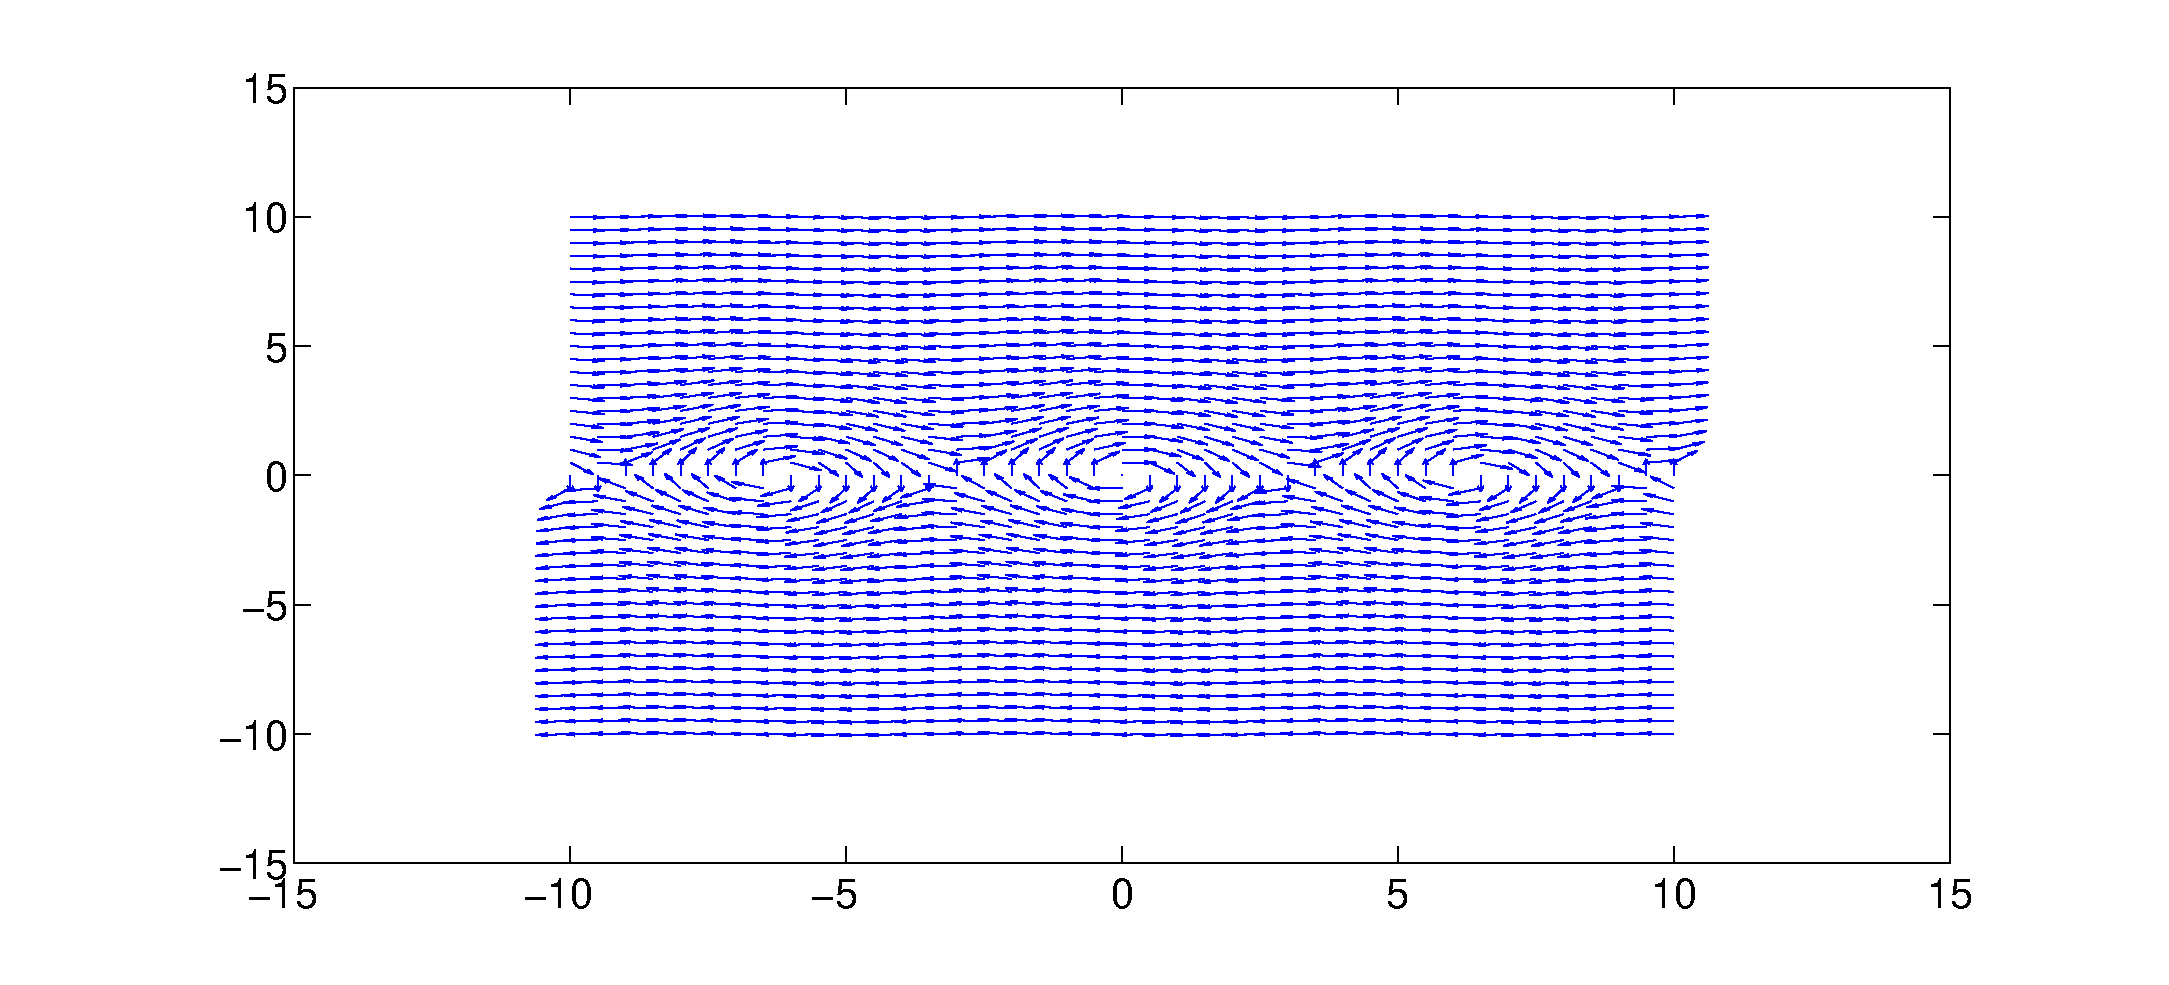
\includegraphics[width=1.0\textwidth]{campo_direzioni_pendolo.eps}
\caption{Campo di direzioni dato da $\mathrm{(SP)}$ con $\omega^2 = 1$.}
\label{T_vs_M}
\end{center}
\end{figure}

Il piano $xy$ è detto anche \emph{piano delle fasi}.  Nel caso $\mathrm{(SP)}$, è facile vedere che i punti di equilibrio (o punti critici) sono dati da
$$
(k\pi,\,0), \qquad k = 0,\, \pm 1,\, \pm 2, \ldots
$$
Pertanto la funzione $x : \mathbb{R} \longrightarrow \mathbb{R}$ definita da
$$
x(t) \doteqdot k\pi, \qquad t \in \mathbb{R}, \; k \text{ fissato in } \mathbb{Z}
$$
è una soluzione di $\mathrm{(EP)}$.

\begin{obs}
Può accadere che due soluzioni si incrocino nel piano $xt$, perché non è detto che abbiano la stessa velocità (hanno derivata prima di $x$ differente).
\begin{center}
\def\svgwidth{8cm}
\input{./04_ODEs/figures/piano_xt_inters.pdf_tex}
\end{center}
Non può invece accadere (per il teorema di esistenza e unicità) che due soluzioni si incontrino in un $t$ finito nel piano delle fasi! A parità di soluzioni, avremmo la stessa velocità! Possono invece toccarsi in un tempo $t$ infinito.
\begin{center}
\def\svgwidth{15cm}
\input{./04_ODEs/figures/piano_xy_inters.pdf_tex}
\end{center}
\end{obs}



\subsubsection{Integrali primi di $\mathrm{(S)}$}
\begin{definition}
Dati $A \subseteq \mathbb{R}^2$ aperto e $f,\,g \in C^1(A)$, una funzione $U \in C^1(A)$ si dice \emph{integrale primo di $\mathrm{(S)}$} nella regione $A$ se
\begin{enumerate}[labelindent=\parindent,leftmargin=*,label=\textnormal{(\roman*)},start=1]
\item $\nabla U(x,\,y) \neq (0,\,0) \qquad \forall (x,\,y) \in A \setminus \lbrace (x,\,y) \in A : f(x,\,y) = g(x,\,y) = 0 \rbrace$
\item Per ogni curva integrale $X : I \longrightarrow \mathbb{R}^2$ di $\mathrm{(S)}$, con $I \subseteq \mathbb{R}$ intervallo, vale
$$
U(X(t)) = U(x(t),\,y(t)) = \text{costante}
$$
\end{enumerate}
\end{definition}


Se in un sistema fisico l'energia si conserva, allora $U$ ha proprio il significato di \emph{energia}. Le curve di livello $\Gamma_c = \lbrace (x,\,y) \in A : U(x,\,y) = c \rbrace$ dove $c \in \mathbb{R}$ costante fissata, si chiamano anche \emph{curve integrali} di $\mathrm{(S)}$.

\begin{obs}[Esercizio 9e, Foglio 7]
Siano $A \subseteq \mathbb{R}^2$ aperto, $f,\,g \in C^1(A)$, e $U \in C^1(A)$ tale che $\nabla U \neq (0,\,0) \qquad \forall (x,\,y) \in A \setminus \lbrace (x,\,y) \in A : f(x,\,y) = g(x,\,y) = 0 \rbrace$. Allora
\begin{center}
$U$ è un integrale primo di $\mathrm{(S)}$
\end{center}
$$
\Updownarrow
$$\vskip 0pt
$$
f(P_0) \frac{\partial U}{\partial x}(P_0) + g(P_0) \frac{\partial U}{\partial y}(P_0) = 0 \qquad P_0 \in A
$$

Tale relazione è facilmente ricavabile osservando che, se $\nabla U \neq (0,\,0)$, la condizione che definisce un integrale primo è
\begin{center}
$\mathrm{(IP)}$
\hfill
$\displaystyle
U(x(t),\,y(t)) = \text{costante}
$
\hfill \null \\
\end{center}
Differenziando $\mathrm{(IP)}$ abbiamo
$$
x'(t_0) \frac{\partial U}{\partial x}(P_0) + y'(t_0) \frac{\partial U}{\partial y}(P_0) = 0 
$$
e, usando $\mathrm{(S)}$,
$$
f(P_0) \frac{\partial U}{\partial x}(P_0) + g(P_0) \frac{\partial U}{\partial y}(P_0) = 0
$$
Questa relazione può anche essere vista nella forma
$$
F(P_0) \bullet \nabla U(P_0) = 0
$$
che appare più intuitiva utilizzando l'interpretazione cinematica. L'orbita della particella è un vincolo dato da $U$, e quindi dal teorema delle funzioni implicite di Dini sappiamo che $\nabla U$ è perpendicolare all'orbita. Poiché $F$, d'altro canto, è tangente all'orbita (rappresenta la velocità!), $\nabla U$ e $F$ sono perpendicolari, ossia il loro prodotto scalare è nullo.
\end{obs}

\begin{thm}
Sia $A \subseteq \mathbb{R}^2$ e sia $U \in C^1(A)$ un integrale primo di $\mathrm{(S)}$. Allora
\begin{enumerate}[labelindent=\parindent,leftmargin=*,label=\textnormal{(\roman*)},start=1]
\item un'orbita $\Gamma \subset A$ di $\mathrm{(S)}$ è contenuta in $\Gamma_c$ per un'opportuna costante $c \in \mathbb{R}$;
\item l'insieme delle curve di livello di $U$ (cioè la famiglia $\Gamma_c = \lbrace (x,\,y) \in A : U(x,\,y) = x \rbrace$ al variare di $c \in \mathbb{R}$) è costituito da un'\emph{unione (disgiunta)} di orbite di $\mathrm{(S)}$.
\end{enumerate}
\end{thm}
\begin{proof}
\mbox{}
\begin{enumerate}[labelindent=\parindent,leftmargin=*,label=\textnormal{(\roman*)},start=1]
\item Sia $\Gamma \subseteq A$ un'orbita di $\mathrm{(S)}$ passante per il punto $(x_0,\,y_0)$, cioè $\Gamma = X(I)$ dove $X : I \longrightarrow \mathbb{R}^2$ è una soluzione di $\mathrm{(S)}$ e $I \subseteq \mathbb{R}$ un intervallo. Fissando $U$ integrale primo di $\mathrm{(S)}$, per definizione vale che
$$
U(X(t)) = U(X(t_0)) = U(x_0,\,y_0) \doteqdot c, \qquad \forall \, t \in I
$$
Quindi $\Gamma_c \subseteq \Gamma$.
\item Sia $c \in \mathbb{R}$ e $\Gamma_c \neq 0$ una curva di livello di $U$. Definiamo
$$
\vartheta_c = \lbrace \Gamma \subseteq \Gamma_c : \Gamma \text{ è un'orbita di } \mathrm{(S)} \rbrace
$$
Dobbiamo provare che
$$
\Gamma_c = \bigcup_{\Gamma \in \vartheta_c} \Gamma
$$
\`{E} banale provare che $\bigcup_{\Gamma \in \vartheta_c} \Gamma \subseteq \Gamma_c$ (già provato al punto $\mathrm{(i)}$). Proviamo quindi che $\Gamma_c \subseteq \bigcup_{\Gamma \in \vartheta_c} \Gamma$. Per il teorema di esistenza e unicità locale di $\mathrm{(PC)}$, otteniamo che $\forall \, (x_0,\,y_0) \in \Gamma_c$, esiste ed è unica un'orbita $\Gamma \in \vartheta_c$ tale che $(x_0,\,y_0) \in \Gamma$. L'unicità ci assicura che l'unione sia disgiunta.
\end{enumerate}
\end{proof}

Ritorniamo al problema di Cauchy da cui siamo partiti
$$
\mathrm{(PCEP)}
\begin{cases}
\; x'' + \omega^2\sin(x) = 0 &\qquad \mathrm{(EP)}\\
\begin{array}{l}
x(t_0) = x_1^0\\
x'(t_0) = x_2^0\\
\end{array}
 &\qquad \mathrm{(CI)}\\
\end{cases}
$$
e al suo sistema associato
$$
\mathrm{(SP)}
\begin{cases}
x' = y\\
y' = -\omega^2\sin(x)\\
\end{cases}
\qquad \qquad
\left(
\begin{array}{rcl}
x(t_0) &=& x_1^0\\
y(t_0) &=& x_2^0\\
\end{array}
\right)
$$
Con l'intento di calcolare l'integrale primo di $\mathrm{(SP)}$ o, equivalentemente, di $\mathrm{(EP)}$, moltiplichiamo ambo i membri di $\mathrm{(EP)}$ per la quantità $ml^2x'$ ottenendo:\footnote{Ricordiamo che $\omega^2 = \dfrac{g}{l}$}
$$
\begin{array}{rcl}
ml^2x'x'' + ml^{\bcancel{2}}x'\dfrac{g}{\bcancel{l}}\sin(x) &=& \\
& \lvert & \\
&=& \dfrac{\mathrm{d}}{\mathrm{d}t}\left( \dfrac{1}{2}ml^2(x')^2 \right) -mlg \dfrac{\mathrm{d}}{\mathrm{d}t}\left( \cos(x) \right)\\
& \lvert & \\
&=& \dfrac{\mathrm{d}}{\mathrm{d}t}\left( \dfrac{1}{2}m(lx')^2 -mgl \cos(x) \right) = 0\\
\end{array}
$$
Definendo le quantità \emph{energia potenziale} ed \emph{energia cinetica} rispettivamente con
$$
E_p \doteqdot mgl(1-\cos(x)), \qquad\qquad E_c \doteqdot \dfrac{1}{2}m(lx')^2
$$
e ponendo
$$
E \doteqdot E_p + E_c
$$
la nostra equazione si riduce a
$$
\dfrac{\mathrm{d}E}{\mathrm{d}t} = 0
\qquad\Longrightarrow\qquad
E = \text{costante}
$$
Abbiamo appena ottenuto la ben nota \emph{legge di conservazione dell'energia}. Utilizzando le $\mathrm{(CI)}$, troviamo
\begin{center}
$\mathrm{(\star)}$
\hfill
$\displaystyle
\dfrac{1}{2}m(lx')^2 - mgl\cos(x) = c_1 = \dfrac{1}{2}m(lx_2^0)^2 - mgl\cos(x_1^0)
$
\hfill \null \\
\end{center}
Dividendo $\mathrm{(\star)}$ per $ml^2$:
$$
\dfrac{1}{2}(x')^2 - \omega^2\cos(x) = c = \dfrac{1}{2}(x_2^0)^2 - \omega^2\cos(x_1^0)
$$
Possiamo quindi definire (ricordando che $y = x'$)
$$
U(x,\,y) = \dfrac{y^2}{2} - \omega^2\cos(x)
$$
\underline{$U$ è un integrale primo di $\mathrm{(SP)}$.} Studiamo ora le sue curve di livello nel piano delle fasi.

Siano $A = \mathbb{R}^2$, $\Gamma_c = \lbrace (x,\,y) \in \mathbb{R}^2 : \dfrac{y^2}{2} - \omega^2\cos(x) = c \rbrace$. Dalla condizione che descrive $\Gamma_c$, abbiamo $c \geq -\omega^2$. Distinguiamo $4$ casi.

\underline{Caso $1$: $c = -\omega^2$}\\
Da $U$, otteniamo
$$
y^2 = 2\omega^2(-1+cos(x))
\qquad\Longleftrightarrow\qquad
(x,\,y) = (2n\pi,\,0) \quad n \in \mathbb{Z}
$$
Dunque $\Gamma_c = \lbrace (2n\pi,\,0) : n \in \mathbb{Z} \rbrace$. Nel piano delle fasi:
\begin{center}
\def\svgwidth{8cm}
\input{./04_ODEs/figures/pendolo_1_fasi.pdf_tex}
\end{center}

\underline{Caso $2$: $-\omega^2 < c < \omega^2$}\\
Da $U$, otteniamo
$$
y^2 = 2(c+\omega^2\cos(x))
\qquad\Longrightarrow\qquad
c+\omega^2\cos(x) \geq 0
\qquad\Longleftrightarrow\qquad
\cos(x) \geq -\dfrac{c}{\omega^2}
$$
Ora, esistono $x_1,\,x_2 \in (-\pi,\,\pi)$ con $-\pi < x_1 < 0 < x_1 < \pi$ tali che
$$
\cos(x) \geq -\dfrac{c}{\omega^2}
\qquad\Longleftrightarrow\qquad
x_1 \leq x \leq x_2
$$
\begin{center}
\def\svgwidth{8cm}
\input{./04_ODEs/figures/pendolo_2_fasi.pdf_tex}
\end{center}

\underline{Caso $3$: $c = \omega^2$}\\
Da $U$, otteniamo
$$
y^2 = 2\omega^2(1+\cos(x))
\qquad\Longleftrightarrow\qquad
\Gamma_c = \lbrace (x,\, \pm \sqrt{2}\omega\sqrt{1+\cos(x)}) : x \in \mathbb{R} \rbrace
$$
Osserviamo che
$$
((2n+1)\pi,\,0) \in \Gamma_c \qquad \forall \, n \in \mathbb{Z}
$$
\begin{center}
\def\svgwidth{8cm}
\input{./04_ODEs/figures/pendolo_3_fasi.pdf_tex}
\end{center}

\underline{Caso $4$: $c > \omega^2$}\\
Da $U$, otteniamo
$$
y^2 = 2\omega^2(c+\cos(x))
\qquad\Longrightarrow\qquad
c+\omega^2\cos(x) > 0 \qquad \forall x \in \mathbb{R}
$$
$$
\Gamma_c = \lbrace (x,\, \pm \sqrt{2}\sqrt{c+\omega^2\cos(x)}) : x \in \mathbb{R} \rbrace
$$
\begin{center}
\def\svgwidth{8cm}
\input{./04_ODEs/figures/pendolo_4_fasi.pdf_tex}
\end{center}

Vediamo ora i possibili grafici delle soluzioni nel piano $tx$ per ogni caso.

\underline{Caso $1$: $c = -\omega^2$}\\
Le soluzioni sono della forma
$$
x(t) = 2n\pi \qquad n \in \mathbb{Z}
$$
In questo caso, abbiamo le cosiddette \emph{soluzioni di equilibrio}:
\begin{center}
\def\svgwidth{8cm}
\input{./04_ODEs/figures/pendolo_1_soluz.pdf_tex}
\end{center}

\underline{Caso $2$: $-\omega^2 < c < \omega^2$}\\
La forma della soluzione è nella figura sottostante. Ma, a questo punto, sorge spontanea la domanda: la soluzione è \emph{periodica}? Cioè, $\exists \, \text{\LARGE $\tau$} \in \mathbb{R}$ ed esiste $x_{\max} : \mathbb{R} \longrightarrow \mathbb{R}$ soluzione di $\mathrm{(EP)}$ tale che
$$
x(t+\text{\LARGE $\tau$}) \qquad \forall \, t \in \mathbb{R}?
$$
Si può provare che, fissate le condizioni iniziali per cui
$$
\begin{cases}
x'' + \omega^2\sin(x) = 0\\
x(t_0) = x_1^0, \quad x'(t_0) = x_2^0
\end{cases}
$$
allora $I_{\max} \equiv \mathbb{R}$ e $x_{\max}$ è periodica.
\begin{center}
\def\svgwidth{8cm}
\input{./04_ODEs/figures/pendolo_2_soluz.pdf_tex}
\end{center}

\underline{Caso $3$: $c = \omega^2$}\\
In questo caso, abbiamo soluzioni di \emph{equilibrio} più soluzioni che \emph{connettono} stati di equilibrio.
\begin{center}
\def\svgwidth{8cm}
\input{./04_ODEs/figures/pendolo_3_soluz.pdf_tex}
\end{center}

\underline{Caso $4$: $c > \omega^2$}\\
Questo è il caso delle cosiddette \emph{soluzioni vorticose}, che hanno un andamento strettamente crescente o decrescente, in quanto
$$
x' = \sqrt{2(c+\omega^2\cos(x))} > 0
$$
\begin{center}
\def\svgwidth{8cm}
\input{./04_ODEs/figures/pendolo_4_soluz.pdf_tex}
\end{center}

Riprendiamo ora il caso $2$, in cui ci eravamo chiesti se la soluzione trovata si potesse ``estendere'' ad una soluzione periodica. Ricordiamo innanzitutto la definizione.

\begin{definition}
Una soluzione $X = (x,\,y) : \mathbb{R} \longrightarrow \mathbb{R}^2$ di $\mathrm{(S)}$ si dice \emph{periodica} se $\exists \, \text{\LARGE $\tau$} \in \mathbb{R}$  tale che
$$
X(t+\text{\LARGE $\tau$}) \qquad \forall \, t \in \mathbb{R}
$$
\end{definition}

La periodicità della soluzione del caso $2$ ci è garantita dal seguente teorema.

\begin{thm}
Sia $A \subseteq \mathbb{R}^2$ aperto e sia $U \in C^1(A)$ un integrale primo di $\mathrm{(S)}$. Definiamo, per un dato $c>0$, 
$$
\Gamma_c \doteqdot \lbrace (x,\,y) \in \mathbb{R}^2 : U(x,\,y) = x \rbrace
$$
e supponiamo che
\begin{enumerate}[labelindent=\parindent,leftmargin=*,label=\textnormal{(\roman*)},start=1]
\item $\Gamma_c$ è una curva \emph{chiusa, regolare e semplice}, cioè, per definizione,
	\begin{itemize}
	\item $\exists \, \varphi : [a,\,b] \longrightarrow A$ di classe $C^1(A)$ e $\varphi'(s) \neq (0,\,0) \quad \forall \, s \in [a,\,b]$ \emph{(regolare)}
	\item $\varphi(a) = \varphi(b)$ \emph{(chiusa)}
	\item $\varphi : [a,\,b] \longrightarrow A$ è iniettiva \emph{(semplice)}	
	\end{itemize}
\item $\Gamma_c$ non contiene punti di equilibrio di $\mathrm{(S)}$
\end{enumerate}
Allora $\Gamma_c$ è un'orbita periodica, cioè, per definizione, esiste $X: \mathbb{R} \longrightarrow \mathbb{R}^2$ soluzione di $\mathrm{(S)}$ periodica e $\Gamma_c = X(\mathbb{R})$.
\end{thm}




\graphicspath{{05_serie_di_fourier/figures/PNG/}{05_serie_di_fourier/figures/PDF/}{05_serie_di_fourier/figures/}}


\chapter{Serie di Fourier}
Le pagine successive sono direttamente a cura del professore. Mi sono solo limitato ad includerle in questo documento.
\pagestyle{plain}
\copyrightnotice
%\includepdf[width=\paperwidth-3cm]{05_serie_di_fourier/Serie_Fourier_12_13.pdf}
\includepdf[width=\paperwidth-1cm]{05_serie_di_fourier/Serie_Fourier_12_13.pdf}


%\appendix
%\renewcommand{\appendixname}{Appendice}
%\chapter{Misure}

%\begin{multicols}{2}
\begin{footnotesize}
%\addcontentsline{toc}{chapter}{Bibliography}
%\bibliographystyle{babalpha}
\bibliographystyle{06_backmatter/math}
\bibliography{06_backmatter/references}
\end{footnotesize}
%\end{multicols}

\end{document}